% !TEX root = ../main.tex
\section{Classical Affine Algebraic Geometry}
\subsection{Introducing Algebraic Sets}
\subsubsection{Introducing Affine Algebraic Sets \& the Affine Zariski Topology}
\begin{definition}\label{AffineSpaceDefinition}
    Let $K$ be any field. By \textit{the affine $n$-space over $K$}, for some positive integer $n$, we mean the $n$-fold cartesian product of $K$ with itself. We denote affine $n$-space over $K$ by $\A^n(K)$ or just $\A^n$ when this will not lead to ambiguity. Thus we have 
    $$\A^n(K) := \A^n := K^n.$$
    We also refer to Affine $1$-space as the affine line, and Affine $2$-space as the affine plane. 
\end{definition}
\begin{remark}
    Whenever we write $\A^n$ and no field is given prior, implicitly a field $K$ is given and we mean $\A^n = \A^n(K)$.
\end{remark}
\begin{definition}\label{VanishingSetDefinition}
    Consider a field $K$. we define \textit{the vanishing set of $S$ over $K$} denoted $V^\A_K(S) := V_K(S):=V(S)$ to be the set
    $$\left\{ v\in \A^n(K) : f(v)=0 \text{ for every } f\in S  \right\}.$$
    similarly we define \textit{the vanishing set of $S$ over $L$} denoted $V_L(S)$ to be the set 
    $$\left\{ v\in \A^n(L) : f(v)=0 \text{ for every } f\in S  \right\}.$$
    When $M$ is finite, say $M= \{f_1,\dots,f_m\}$, we define 
    $$V_F(f_1,\dots,f_m) := V_F(\{f_1,\dots,f_m\}) \quad V_L(f_1,\dots,f_m) := V_L(\{f_1,\dots,f_m\}).$$
    Our convention will be that $V(M):=V_K(M)$
\end{definition}

\begin{definition}\label{AlgebraicSubsetDefinition}
    Let $K$ be any field. A subset $X \subset \A^n$ is called an \textit{affine algebraic subset}, or an \textit{algebraic subset} when no ambiguity arises, if there is a subset $M\subset K[x_1,\dots,x_n]$ such that $X = V(M)$ 
\end{definition}

\begin{lemma}\label{SetSupersetImpliesVanishingSetOfSetSubsets}
    Let $M,M'\subset K[x_1,\dots,x_n]$ with $M\supset M'$. Then $V(M)\subset V(M')$.
\end{lemma}
\begin{proof}
    Let $v\in V(M)$ and $f\in M'$. Then by assumption $f\in M$ and hence $f(v)=0$, implying $v\in V(M')$. 
\end{proof}
\begin{proposition}\label{EveryVanishingSetIsAVanishingSetOverIdeal}
    For any subset $M\subset K[x_1,\dots,x_n]$. Set $I:= \langle M\rangle$. Then $V(M)=V(I)$
\end{proposition}
\begin{proof}
    Let $v\in V(M)$. Let $f\in I$. Then for some $f_1,\dots,f_m\in S$ 
    $$f = \sum_1^m c_if_i,$$
    for suitable $c_1,\dots,c_m\in K[x_1,\dots,x_n]$. Then $f_i(v) = 0$ for every $i\in\{1,\dots,m\}$ and hence 
    $$f(v)=\sum_1^m c_i(v)f_i(v) = \sum_1^m c_i(v)\cdot 0 = 0,$$
    meaning $v\in V(I)$ and hence $V(M)\subset V(I)$.\\
    The converse inclusion follows from Lemma~\ref{SetSupersetImpliesVanishingSetOfSetSubsets} since $I\supset M$.  
\end{proof}
It follows as a corollary that every affine algebraic set arises as a vanishing of some polynomial ideal.
\begin{corollary}\label{AlgebraicSubsetArisesAsVanishingSetOfIdeal}
    Let $X\subset \A^n$ be algebraic. Then $X=V(I)$ for some ideal $I\subset K[x_1,\dots,x_n]$.
\end{corollary}
As another corollary to the above proposition we have that every algebraic set arises as . 
\begin{corollary}\label{AlgebraicSubsetArisesAsVanishingSetOfFiniteSet}
    Let $X\subset \A^n$ be an algebraic subset. Then $X = V(f_1,\dots,f_m)$ for suitable $f_1,\dots,f_m\in K[x_1,\dots,x_n]$.
\end{corollary}
\begin{proof}
    By Corollary~\ref{AlgebraicSubsetArisesAsVanishingSetOfIdeal} $X=V(I)$ for some ideal $I\subset K[x_1,\dots,x_n]$. By Corollary~\ref{PolynomialIdealOverFieldIsFinitelyGenerated} $I=\langle f_1,\dots,f_m\rangle$ for suitable $f_1,\dots,f_m\in K[\mathbf{x}]$. Thus it follows from the above proposition that
    $$X= V(I) = V(\langle f_1,\dots,f_m\rangle)= V(f_1,\dots,f_m).$$
\end{proof}
\begin{remark}\label{AlgebraicSubsetIsZeroSetOfPolynomialMap}
    Let an algebraic subset $X\subset \A^n$ be given. We can find $f_1,\dots,f_m\in K[x_1,\dots,x_n]$ such that $X=V(f_1,\dots,f_m)$. Consider the map 
    \begin{gather*}
        \varphi: \A^n \rightarrow \A^m\\
        v\mapsto \left(\ev_v(f_1),\ev_v(f_2),\dots,\ev_v(f_m)\right) = (f_1(v),f_2(v),\dots,f_m(v)).
    \end{gather*}
    It is then clear that $V(f_1,\dots,f_m)=\varphi^{-1}(\textbf{0})$. Thus one concludes that every algebraic subset of $\A^n$ arises the zero set of a map of the same form as $\varphi$. We shall later see that $\varphi$ is an element of a special class of maps, called \textit{polynomial maps}, which are central to study of affine algebraic geometry. 
\end{remark}
\begin{lemma}\label{AlgebraicSubsetsAreClosedUnderIntersectionAndFiniteUnion}
    We collect the following results
    \begin{enumerate}[(i)]
        \item Let $A$ be some indexing set. Consider a family of algebraic sets $\{X_\alpha\}_{\alpha\in A}$ in $\A^n$. Then $\bigcap_{\alpha} X_\alpha$ is an algebraic set.
        \item Consider algebraic sets $X,Y\subset \A^n$. Then $X\cup Y$ is algebraic. It follows by induction that $\bigcup_1^k X_i$ is algebraic for any finite sequence of algebraic sets $X_1,\dots,X_k$ in $\A^n$.  
    \end{enumerate}
\end{lemma}
\begin{proof}
    (i) By Corollary~\ref{AlgebraicSubsetArisesAsVanishingSetOfIdeal} for every $\alpha\in A$, we can find an ideal $I_\alpha \subset K[x_1,\dots,x_n]$ such that $X_\alpha = V(I_\alpha)$. We claim that $\bigcap_\alpha V(I_\alpha) = V\left( \bigcup_\alpha I_\alpha\right)$.\\
    Let $v \in \bigcap_\alpha V(I_\alpha)$. Let $f\in \bigcup_\alpha I_\alpha$. Then $f\in I_\beta$ for some $\beta\in A$. Then since $v \in \bigcap_\alpha V(I_\alpha)$, in particular $v\in V(I_\beta)$, implying $f(v) = 0$, hence $v\in V\left( \bigcup_\alpha I_\alpha\right)$.\\
    Let $\beta\in A$, then $I_\beta \subset \bigcup_\alpha I_\alpha$. By Lemma~\ref{SetSupersetImpliesVanishingSetOfSetSubsets} $V\left(\bigcup_\alpha I_\alpha\right) \supset V(I_\beta)$, hence $V\left(\bigcup_\alpha I_\alpha\right) \supset \bigcap_\alpha V(I_\alpha)$.\\
    It follows that 
    $$\bigcap_\alpha X_\alpha =\bigcap_\alpha V(I_\alpha) = V\left(\bigcup_\alpha I_\alpha\right).$$
    (ii) We have that $X= V(I)$ and $Y = V(J)$ for some ideals $I,J\subset K[x_1,\dots,x_n]$. We claim that $V(I)\cup V(J) = V(IJ)$.\\ 
    $IJ\subset I$ and $IJ \subset J$, hence by Corollary~\ref{SetSupersetImpliesVanishingSetOfSetSubsets} $V(I),V(J)\subset V(IJ)$, meaning $V(I)\cup V(J) \subset V(IJ)$.\\
    Let $v\in V(IJ)$. If $v\in V(I)$ we find that $v\in V(I)\cup V(J)$. Suppose $v\notin V(I)$. Then for some $f\in I$ $f(v)\neq 0$. Let $g\in J$ be given. then $fg\in IJ$, hence $0 = (fg)(v) = f(v)g(v)$, since $f(v)\neq 0$ it follows that $g(v)= 0$, hence $v\in V(J)\subset V(I)\cup V(J)$.\\
    It follows that 
    $$X\cup Y = V(I)\cup V(J) = V(IJ).$$
\end{proof}
We collect the most fundamental examples of (affine) algebraic sets
\begin{example}\label{FundamentalExmaplesOfAffineAlgebraicSubsets}
Fix a field $K$
    \begin{enumerate}
        \item Trivially the vanishing set of some subset $M\subset K[x_1,\dots,x_n]$ is a an algebraic set. 
        \item Affine $n$-space is an algebraic set. Indeed, see that 
        $$\A^n = V(0)$$
        \item The empty set $\emptyset\subset \A^n$ is an algebraic set. Indeed one readily verifies that
        $$\emptyset = V(1).$$
        \item A singleton or \textit{point}, $\{(a_1,\dots,a_n)\}$ for $a_1,\dots,a_n\in K$, is an algebraic set. Indeed, one checks that
        $$\{(a_1,\dots,a_n)\} = V(x_1-a_1,\dots,x_n-a_n).$$
        It thus follows that from Lemma~\ref{AlgebraicSubsetsAreClosedUnderIntersectionAndFiniteUnion} (ii) that any finite subset of $\A^n$ is algebraic
    \end{enumerate}
\end{example}
We can represent some of the data collected thus far as a topology on affine $n$-space
\begin{theorem}
    Consider the family of sets 
    $$\tau_\mathcal{Z} := \left\{ \A^n\setminus X : X\subset \A^n \text{ is an algebraic set} \right\}.$$
    This constitutes a topology on $\A^n$ called the \textit{Zariski topology}. 
\end{theorem}
\begin{proof}
    One sees from example~\ref{FundamentalExmaplesOfAffineAlgebraicSubsets} 2. \& 3. that $\A^n,\emptyset \in \tau_\mathcal{Z}$.\\
    Consider some indexing set $A$. Let $\{B_\alpha\}_{\alpha\in A}\subset \tau_\mathcal{Z}$ be given. For each $\alpha\in A$ we can find $X_\alpha\subset \A^n$ such that $B_\alpha =\A^n\setminus X_\alpha.$ Then it follows from Proposition~\ref{AlgebraicSubsetsAreClosedUnderIntersectionAndFiniteUnion} (i) that
    $$\bigcup_\alpha B_\alpha = \bigcup_\alpha \A^n\setminus X_\alpha = \A^n\setminus \left(\bigcap_\alpha X_\alpha \right) \in \tau_\mathcal{Z}$$
    Let $B_1,\dots,B_k\in \tau_\mathcal{Z}$. For suitable $X_1,\dots,X_k\subset \A^n$, $B_i = \A^n\setminus X_i$. Then it follows from Proposition~\ref{AlgebraicSubsetsAreClosedUnderIntersectionAndFiniteUnion} (ii) that
    $$\bigcap_1^k B_i = \bigcap_1^k \A^n\setminus X_i = \A^n\setminus \left(\bigcup_1^k X_i\right)\in \tau_\mathcal{Z}.$$  
\end{proof}
\begin{remark}
    The closed subsets of $\A^n$ under the Zariski topology are exactly the algebraic sets in $\A^n$. Thus we may opt to say that an algebraic subset $X\subset \A^n$ is a \textit{Zariski closed subset}. 
\end{remark}
\subsubsection{Miscellaneous Result about Algebraic sets, Examples \& Non-examples}
\begin{proposition}\label{AlgebraicSubsetsOfAffine1SpaceAreFiniteSetsAndTheWholeSpace}
    The Zariski closed subsets of $\A^1=K$ are the finite subsets of $\A^1$ and $\A^1$ itself.  
\end{proposition}
\begin{proof}
    Let $X\subset \A^1$ be Zariski closed. Suppose $X\neq V(0)=\A^1$, i.e. that $X = V(f_1,\dots,f_m)$ for $f_1,\dots,f_m\in K[x_1,\dots,x_n]$, where $f_i \neq 0$ for at least one $i\in\{1,\dots,m\}$.  Then $X\subset V(f_i)$ by Lemma~\ref{SetSupersetImpliesVanishingSetOfSetSubsets}.  $V(f_i)$ is the set of roots of $f_i$. Since $f_i\neq 0$, $\# V(f_i) \leq \deg \ f_i < \infty$ {\LARGE GIVE REFERENCE}, hence 
    $$\#X\leq \#V(f_i)\leq \deg \ f_i<\infty.$$
\end{proof}

\begin{proposition}\label{EverySubsetOfFiniteAffineSpaceIsAlgebraic}
    Let $K$ be a field with $\# K <\infty$. Let $X\subset \A^n$. Then $X$ is Zariski closed. 
\end{proposition}
\begin{proof}
    By assumption $\#X < \infty$, hence there are points $v_1,\dots,v_k\in \A^n$ such that 
    $$X = \bigcup_1^k \{v_i\}.$$
    By Example~\ref{FundamentalExmaplesOfAffineAlgebraicSubsets} $X$ is Zariski closed. 
\end{proof}
We now give an example of a countable family of algebraic subsets whose union is not algebraic. 
\begin{example}\label{ExampleOfCountableUnionOfAlgebraicSubsetsWhichIsNotAlgebraic}
    Let $K=\Q$ and let and consider the family of algebraic sets $\{ \{i\}\}_{i\in \N}$. The only algebraic subset of $\A^1$ are $\A^1$ it self and the finite subsets of $\A^1$ (cf. Proposition~\ref{AlgebraicSubsetsOfAffine1SpaceAreFiniteSetsAndTheWholeSpace}), but $\bigcup_{i\in \Z} \{i\} = \Z$, which is neither finite or equal to $\A^1=\Q$. 
\end{example}
Here are some examples of algebraic subsets
\begin{example}\label{ExamplesOfAlgebraicSets}
    \begin{enumerate}
        \item Let $X=\left\{\left(t,t^2,t^3\right)\in \A^3 : t\in K\right\}$. We prove that $X= V\left(f_1,f_2\right)$, where $f_1=x^2-y,f_2=x^3-z\in K[x,y,z]$. Let $v\in X$. Then $v=(t,t^2,t^3)$ for some $t\in K$. Note that 
        $$f_1(v)=t^2-t^2=0 \text{ and } f_2(v)=t^3-t^3=0,$$
        implying that $v\in V(f_1,f_2).$\\
        Let $v=(v_1,v_2,v_3)\in V(f_1,f_2)$. Put $t = v_1$. Then $t^2 = v_1^2 = v_2$ and $t^3 = v_1^3=v_3$, hence $v=(v_1,v_2,v_3)=(t,t^2,t^3)\in X$.
        \item Let $X = \left\{(\cos(t),\sin(t))\in \A^2(\R) : t\in \R\right\}$.  One sees that $X= V(x^2+y^2-1)$. Indeed, for $v=(\cos(t),\sin(t))\in X$, $\sin^2(t)+\cos^2(t)=1,$ implying that $v\in V(x^2+y^2-1).$ For $v=(v_1,v_2)\in V(x^2+y^2-1)$, we have that $\vert v\vert^2 =v_1^2+v_2^2 = 1$, implying that $v\in S^1 = \text{im}(\R \ni t \mapsto (\cos(t),\sin(t)\in \A^2(\R))$.
        \item Let $X=\left\{ \left(\sin(t)\cos(t),\sin^2(t)\right)\in \A^2(\R) : t\in [0,2\pi)\right\}$, i.e. the points in $\A^2(\R)$ with polar coordinates $(r,t)$ such that $r=\sin(t)$. Recall the trigonometric identities
        \begin{align*}
            &\sin(\alpha+\beta) = \sin(\alpha)\cos(\alpha) +\sin(\beta)\cos(\alpha),\\
            &\cos(\alpha+\beta) = \cos(\alpha)\cos(\beta)-\sin(\alpha)\sin(\beta)
        \end{align*}
        for $\alpha,\beta\in [0,2\pi)$. For $t\in [0,2\pi)$ this is equivalent to 
        \begin{align*}
            &\sin(2t)= 2\sin(t)\cos(t) \iff \sin(t)\cos(t)=\frac{1}{2}\sin(2t) \text{ and }\\
            &\cos(2t) = \cos^2(t)-\sin^2(t) = 1-2\sin^2(t) \iff \sin^2(t)=\frac{1}{2}\left(1-\cos(2t)\right),
        \end{align*}
        hence $X = \left\{ \left(\frac{1}{2}\sin(2t),\frac{1}{2}\left(1-\cos(2t)\right)\right) : t \in [0,2\pi)\right\}.$ Let $f = x^2 + \left(\frac{1}{2}-y\right)^2-\frac{1}{4}$. One sees that $X= V(f)$. Indeed, if $v=(\left(\frac{1}{2}\sin(2t),\frac{1}{2}\left(1-\cos(2t)\right)\right)\in X$ we have that 
        $$f(v)=\frac{1}{4}\cos^2(2t)+\left(\frac{1}{2}-\frac{1}{2}+\frac{1}{2}\sin(2t)\right)^2-\frac{1}{4} =\frac{1}{4}\left(\cos^2(2t)+\sin^2(2t)\right)-\frac{1}{4}=\frac{1}{4}-\frac{1}{4}=0,$$
        thus we conclude $v\in V(f).$ Let $v=(v_1,v_2)\in V(f)$. We set $t=\frac{1}{2}\arcsin(2v_1)$. Then one easily checks that $\cos(2t)=v_1$. We also note that 
        $$v_1^2=-\left(\frac{1}{2}-v_2\right)^2+\frac{1}{4}.$$
        Therefor we get that
        \begin{align*}
        \frac{1}{2}(1-\cos(2t))&=\frac{1}{2}\left(1-\cos\left(2\frac{1}{2}\arcsin(2v_1)\right)\right) = \frac{1}{2}\left(1-\sqrt{1-4v_1^2}\right)\\
        &=\frac{1}{2}\left(1 -\sqrt{1+4\left(\left(\frac{1}{2}-v_2\right)^2-\frac{1}{4} \right)} \right)=\frac{1}{2}\left(1-\sqrt{1-1+4\left(\frac{1}{2}-v_2\right)^2}\right)\\
        &= \frac{1}{2}\left(1-2\left(\frac{1}{2}-v_2\right) \right)=\frac{1}{2}\cdot 2v_2=v_2.
        \end{align*}
        \noindent Hence $v=(v_1,v_2)=\left(\frac{1}{2}\sin\left(2t\right),\frac{1}{2}\left(1-\cos\left(2t\right)\right) \right)\in X$
        \newpage
        \begin{figure}[h]
            \centering
            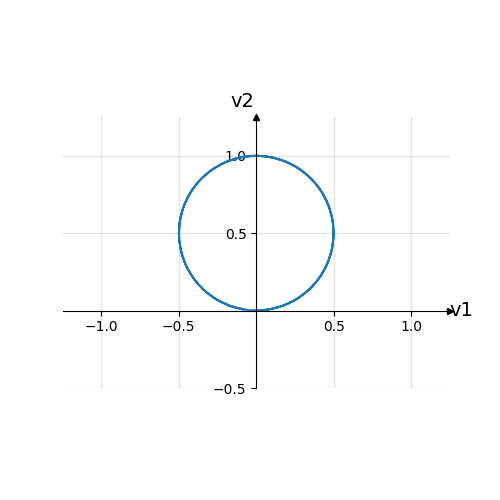
\includegraphics[scale = 1]{figures/AlgebraicCurveEx3.png}
            \caption{The algebraic curve given by $V(x^2-(1/2-y)^2-1/4)$ is a circle of radius $1/2$ and center $(0,1/2)$}
            \label{fig:AlgebraicCurveEx}
        \end{figure}
    \end{enumerate}
\end{example}

\begin{definition}
    An algebraic subset of an $\A^2$ is called an \textit{algebraic curve}.
\end{definition}
\begin{definition}
    The vanishing set of a non-zero polynomial $f\in K[x_1,\dots,x_n]$ is called a \textit{hypersurface}. If $\deg \ f = 1$, then its vanishing set is called a \textit{hyperplane}. 
\end{definition}
\begin{definition}
    A hypersurface in $\A^2$ is called an \textit{affine plane curve}. A hyperplane in $\A^2$ is called a \textit{line}.
\end{definition}
\begin{remark}
    Consider a line $V(f)\subset \A^2$, where $f=ax+by+c$, for $a,b,c\in K$ where $a$ or $b$ are non-zero. Without loss of generality we may assume that $b\neq 0$. Thus 
    $$V(f)= V(f)\cup \emptyset = V(f)\cup V\left(b^{-1}\right) = V\left(b^{-1}(ax+by+c)\right)=V\left(y+ab^{-1}x+cb^{-1}\right).$$
    This means that any can be expressed as the vanishing set of some polynomial of the form 
    $$y-Ax+B,$$
    for some $A,B\in K.$
\end{remark}

\begin{proposition}\label{LineIntersectsAffinePlaneCurveOnlyFinitelyManyTimes}
    Consider $l = y-(ax+b)\in K[x,y]$ and a line $L=V(l)$ and an affine plane curve $C =V(f),$ where $f\in K[x,y]$ with $n=\deg\ f$ such that $L\not\subset C$. Then $C\cap L$ is a finite set containing at most $n$ points.
\end{proposition}
\begin{proof}
    The case where $\#K < \infty$ is trivial. Suppose then that $\#K = \infty$.
    Set
    $$X := \{(t,at+b)\in \A^2 : f(t,at+b)=0\}.$$
    Note that $t \in V(f(x,ax+b))$ if and only if $(t,at+b)\in X$ and thus that there is a $t \in \A^1\setminus V(f(x,ax+b)$, since $L\not\subset C$. This then implies that  $\#V(f(x,ax+b))\leq n$ (cf. Example~\ref{AlgebraicSubsetsOfAffine1SpaceAreFiniteSetsAndTheWholeSpace}), and hence $\#X \leq n$. It is then sufficient to prove that $C\cap L = X$. Let $v=(v_1,v_2)\in C\cap L$. Since $v\in L$ we have that 
    $$v_2 = av_1+b,$$
    meaning $v=(v_1,v_2)=(v_1,av_1+b)\in X$. Conversely, let $v=(t,at+b)\in X$. Then 
    $$l(v) = at+b-(at+b) = 0,$$
    hence $v\in L$. Clearly we also have that $v\in C$, meaning $v\in C\cap L$.
\end{proof}
\begin{corollary}\label{LineIntersectsAlgebraicCurveOnlyFinitelyManyTimes}
    An algebraic curve $X\subset \A^2$ intersects a line $L$ not contained in $X$ in only finitely many points.
\end{corollary}
\begin{proof}
    $X=V(f_1,\dots,f_m)$, for some $f_1,\dots,f_m\in K[x,y]$, where without loss of generality $f_1\neq 0$. Then $X\subset V(f_1)$ and $L \not\subset V(f_1)$, which by Proposition~\ref{LineIntersectsAffinePlaneCurveOnlyFinitelyManyTimes} implies that $\#X\leq \#V(f_1)\leq \deg\ f_1 <\infty$.
\end{proof}
We use this result to give some non-examples of algebraic subsets
\begin{example}
    \begin{enumerate}
        \item Consider the graph of the sine function,
        $$G := \{(t,\sin(t))\in \A^2(\R) : t\in \R \}$$
        Consider also the line $L:=V(y)$. One easily verifies that $L=\{(t,0)\in \A^2(\R) : t\in \R\}$. Thus $G\cap L = \{ (n\pi,0)\in \A^2(\R) : n\in \Z\} \neq L,$ hence $\#(G\cap L) = \infty$, and $G$ is not algebraic by Corollary~\ref{LineIntersectsAlgebraicCurveOnlyFinitelyManyTimes}.
        \item Consider the sphere
        $$S:=\left\{(z,w)\in \A^2(\C) : \vert z \vert^2+\vert w \vert^2 = 1 \right\}.$$
        Consider again the line $L:=V(y)$. Note that $S\cap L  = \left\{ (z,0) \in \A^2(\C) : \vert z\vert = 1 \right\} \neq L$ and that this set is in bijection with $S^1$. But clearly $\#S^1=\infty$, hence $S$ cannot be algebraic by Corollary~\ref{LineIntersectsAlgebraicCurveOnlyFinitelyManyTimes}.
    \end{enumerate}
\end{example}
\begin{definition}
    Given an algebraic set $X\subset \A^n$ and $(b_1,\dots,b_n)\in\A^n$, a \textit{translation} is a map 
    \begin{gather*}
        \varphi: X \rightarrow \A^n\\ (v_1,\dots,v_n)\mapsto (v_1+b_1,\dots,v_n+b_n)
    \end{gather*}
\end{definition}
\begin{lemma}\label{AlgebraicSetsAreCloseUnderTranslation}
    Algebraic sets are closed under translation. In other words, let $X:=V(f_1,\dots,f_m)\subset \A^n$ be an algebraic set. Let $b_1,\dots,b_n\in K$. Then the image of the map 
    \begin{gather*}
        \varphi : X \rightarrow \A^n\\
        (v_1,\dots,v_n)\mapsto (v_1+b_1, \dots, v_n+b_n)
    \end{gather*}
    is an algebraic set
\end{lemma}
\begin{proof}
    One checks that $\text{im } \varphi = V(f_1(x_1-b_1,\dots, x_n-b_n),\dots,f_m(x_1-b_1,\dots, x_n-b_n))$. Indeed, let 
    $(v_1+b_1,\dots,v_n+b_n)\in \text{im } \varphi$. Then 
    $$f_i(v_1+b_1-b_1,\dots,v_n+b_n-b_n)=f_i(v_1,\dots,v_n) = 0.$$
    On the other hand, let 
    $$(v_1,\dots,v_n) \in V(f_1(x_1-b_1,\dots, x_n-b_n),\dots,f_m(x_1-b_1,\dots, x_n-b_n)),$$
    Then $(v_1-b_1,\dots,v_n-b_n)\in V(f_1,\dots,f_n)$ and 
    $$(v_1,\dots,v_n) = \varphi(v_1-b_1,\dots,v_n-b_n) \implies (v_1,\dots,v_n)\in \text{im }\varphi.$$
\end{proof}
\begin{lemma}\label{AlgebraicSetsAreClosedUnderPermutation}
    Let $X\subset \A^n$ be algebraic and $\omega\in \pazocal{S}_n$. Then the image of 
    \begin{gather*}
        \varphi: X\rightarrow \A^n\\
        (v_1,\dots,v_n)\mapsto (v_{\omega(1)},\dots,v_{\omega(n)})
    \end{gather*}
    is algebraic.
\end{lemma}
\begin{proof}
    For suitable $f_1,\dots,f_m\in K[x_1,\dots,x_n]$, $X=V(f_1,\dots,f_m)$. Clearly, 
    $$\mathrm{im}\ \varphi = V\left(f_1\left(x_{\omega^{-1}(1)},\dots,x_{\omega^{-1}(n)}\right),\dots,f_m\left(x_{\omega^{-1}(1)},\dots,x_{\omega^{-1}(n)}\right)\right).$$
    Indeed, if $w=(v_{\omega(1)},\dots,v_{\omega(n)})\in \mathrm{im}\ \varphi$. Then 
    $$f_i\left(w_{\omega^{-1}(1)},\dots,w_{\omega^{-1}(n)}\right)=f_i\left(v_{\omega^{-1}(\omega(1))},\dots,v_{\omega^{-1}(\omega(n))}\right)=f_i(v_1,\dots,v_n)=0.$$
    Conversely, if $v=(v_1,\dots,v_n)$ is an element of the right-hand side, then picking $w=\left((v_{\omega^{-1}(1)},\dots,v_{\omega^{-1}(n)} \right)$, then $f_i(w)=0$ and $\varphi(w)=v$.
\end{proof}
\begin{definition}\label{GeneralDefinitionOfALine}
    We define a \textit{line} in $\A^n$ given by $a_1,\dots,a_n,b_1,\dots,b_n\in K$, where $a_j \neq 0$ for some $j$ to be the set 
    $$\left\{ \begin{pmatrix} a_1t + b_1\\ \vdots \\ a_nt+b_n \end{pmatrix}\in\A^n : t \in K \right\}$$
\end{definition}
\begin{lemma}\label{LineIsZariskiClosed}
    A line in $\A^n$ is Zariski closed. 
\end{lemma}
\begin{proof}
    We consider first the case where $a_1\neq0$. It is easy to check that 
    $$V(\{a_1x_i - a_ix_1-a_1b_i+a_ib_1 : i\neq 1\}) = \left\{ \begin{pmatrix} a_1t+b_1\\ a_2t+b_2\\ \vdots \\ a_nt+b_n \end{pmatrix}\in\A^n : t \in K \right\}.$$
    Any other line can be obtained as the image translation composed with a map induced by a permutation of a line of the above form, hence by Lemmas~\ref{AlgebraicSetsAreCloseUnderTranslation} and \ref{AlgebraicSetsAreClosedUnderPermutation} any line is Zariski closed.
\end{proof}
The intersection of a proper configuration of $n-1$ hyperplanes is a line for $n\geq 2$.
\begin{proposition}
    Consider a hyperplanes $V(p_1+b_i),\dots,V(p_{n-1}+c_{n-1})$, with $p_i = \sum_1^n a_{ij}x_j\in K[x_1,\dots,x_n]$, $b_i\in K$ such that the vectors 
        $$a_i:=\begin{pmatrix}
            a_{i1}\\
            \vdots\\
            a_{in}
        \end{pmatrix}, \quad (i\in \{1,\dots,n-1\}) $$
    are linearly independent. The intersection of these hyperplanes, $L$ say, is a line.     
\end{proposition}
\begin{proof}
    Our assumptions lets us show that WLOG
    \begin{align*}
        L = \left\{ v\in \A^n : \begin{pmatrix}
            a_{11} & \cdots & a_{1n}\\
            \vdots & \ddots & \vdots\\
            a_{(n-1) 1} & \cdots & a_{(n-1) n}\\
            0 & \cdots & 0
        \end{pmatrix} v = \begin{pmatrix} b_1\\ \vdots\\ b_{n-1} \\0 \end{pmatrix}\right\} = \left\{ v\in \A^n : \begin{pmatrix}
            c_{ij} 
        \end{pmatrix} v = \begin{pmatrix}
            b_1' \\ \vdots \\ b_{n-1}' \\0
        \end{pmatrix} \right\} 
    \end{align*}
    where $c_{ii} = 1$ for $i\in \{1,\dots, n-1\}$, $c_{nn}=0$ and $c_{ij}=0$ for $i,j\in \{1,\dots,n\}$ where $i>j$ and $n>j>i$. In other words 
    $$L = \bigcap_1^{n-1} V(x_i-c_ix_n-b_i'),$$
    for suitable $c_i'b_i'\in K$. This means that 
    $$L = \{(c_1t+b_1',\dots,c_{n-1}t+b_{n-1}',t) \in \A^n : t \in K\}.$$   
\end{proof}
We can extend the result in Proposition~\ref{LineIntersectsAffinePlaneCurveOnlyFinitelyManyTimes} in the following way
\begin{proposition}\label{NumberOfIntersectionsOfAlgebraicSetWithLine}
     Consider also a hypersurface $H:=V(f)\subset \A^n$ with $d:=\deg f >0$ and a line $L\subset \A^n$ with $n\geq 2$ such that $L\not\subset H$. Then $\#(L\cap H) \leq d$ 
\end{proposition}
\begin{proof}
    For suitable $a_1,\dots,a_n,b_1,\dots,b_n\in K$ with $a_j\neq 0$ for some $j$ we have that 
    $$ L = \left\{ \begin{pmatrix}
        a_1t+b_1\\ \vdots\\ a_nt+b_n
    \end{pmatrix}\in \A^n : t\in K \right\}$$
    We may then easily prove that 
    $$L \cap H = \left\{ (a_1t+b_1,\dots,a_nt+b_n)\in \A^n : f(a_1t+b_1,\dots,a_nt+b_n)= 0 \right\}$$
    and that $(a_1t+b_1,\dots,a_nt+b_n)\in L\cap H$ if and only if 
    $$t \in V(f(a_1x+b_1,\dots,a_nx+b_n)).$$
    Since $L \cap H \neq L$, there is a $t \in \A^1$ such that $t \notin V(f(a_1x+b_1,\dots,a_nx+b_n))$, hence
    $$\#(L\cap H) = \#V(f(a_1x+b_1,\dots,a_nx+b_n)) \leq d$$
\end{proof}
\begin{corollary}\label{AlgebraicSetCanIntersectLineOnlyFinitely}
     Consider a line $L\in \A^n$. Then $L$ intersects any algebraic set not containing $L$ only finitely many times. 
\end{corollary}
\begin{example}
    Consider the helix 
        $$H := \left\{(\cos(t),\sin(t),t)\in \A^3(\R) : t\in \R \right\}.$$
    Consider also the line $L:=\{ (0,1,t)\in \A^3(\R) : t \in \R\}$ and note that $L \cap H = \{ (0,1, 2n\pi + \pi/2) : n\in \Z\}\neq \A^1$, but we also have that $\# L\cap H = \infty$, hence $H$ cannot be algebraic by \ref{AlgebraicSetCanIntersectLineOnlyFinitely}.
\end{example}
\begin{proposition}\label{AlgebraicSetsOverInfiniteFieldsAndAlgClosedFields}
    Suppose $K$ is an infinite field. Let $f\in K[x_1,\dots,x_n]$ with $\deg \ f>0$
    \begin{enumerate}
        \item Suppose $n\geq 1$. Then $\#\left(\A^n\setminus V(f)\right) = \infty$.
        \item Suppose that $K$ is algebraically closed and that $n\geq 2$. Then $\#V(f) = \infty$
    \end{enumerate}
\end{proposition}
\begin{proof}
    1. In the one variable case every algebraic subset that is not affine $n$-space is finite, hence $\#\left(\A^1\setminus V(f) \right) = \infty$. Suppose then that $n\geq 2$. Since $f$ is non-constant, we can write (cf. {\large ref})
    $$f = \sum_0^d f_ix_n^{i},$$
    for a $d\geq 1$ and for suitable $f_i\in K[x_1,\dots,x_{n-1}]$ with $f_j \neq0$ for some $j\in \{1,\dots,d\}$. By Proposition~\ref{OnInfiniteFieldPolynomialVanishesEverywhereIfAndOnlyIfIsZero} there is a point $v\in \A^{n-1}$ such that $f_j(v)\neq 0$. Hence 
    $$f' := \sum_0^d f_i(v)x_n^i\in K[x_n]$$
    is a non-zero polynomial in one variable, implying that that that for every infinitely many $v_n\in K$ such that $f'(v_n)=f(v_1,\dots,v_n)\neq 0$, hence $\A^n\setminus V(f)$ is infinite.\\
    2. We again write $f=\sum_0^d f_ix_n^i$, for suitable $f_i\in K[x_1,\dots,x_{n-1}]$, with $f_j\neq 0$ for some $j\in\{1,\dots,d\}$. If every non-zero $f_i$ is constant, then for any choice of $v\in \A^n$, there exists $a_v\in K$ such that for $f_v = \sum_0^d f_i(v)x_n^i$, 
    $$0 = f_v(a_v) = f(v_1,\dots,v_{n-1},a_v).$$
    If $\deg \ f_j >0$ for some $j$. Then there are infinitely many $v\in \A^{n-1}$ such $f_j(v)\neq 0$. For such a $v$ there is at least one $a_v\in K$ that is a root in $f(v_1,\dots,v_{n-1},x_n)$. Thus in any case $f$ has infinitely many zeroes, i.e. $V(f)$ is infinite.
\end{proof}
We present a way of constructing algebraic sets via Cartesian product
\begin{proposition}
    Let $X\subset \A^n$ and $Y\subset \A^m$ be algebraic then. $X\times Y \subset \A^{n+m}$ is algebraic.
\end{proposition}
\begin{proof}
    For suitable $f_1,\dots,f_k \in K[x_1,\dots,x_n]$  and $g_1,\dots, g_l \in K[y_1,\dots,y_m]$, we have $X = V(f_1,\dots,f_m)$ and $Y=V(g_1,\dots,g_l)$. We prove that $X\times Y = V(f_1,\dots,f_k,g_1,\dots,g_l)$, where we consider $f_1,\dots,f_k,g_1,\dots,g_l$ as elements of $K[x_1,\dots,x_n,y_1,\dots,y_m]$. Let $(v,w)\in X\times Y$. then clearly $f_i(v,w) = 0$ and $g_j(v,w)=0$ for every $i\in\{1,\dots,k\}$ and every $j\in\{1,\dots, l\}$. Let $(v,w)\in V(f_1,\dots,f_k,g_1,\dots,g_l)$. Considering $f_1,\dots,f_k$ and $g_1,\dots,g_l$ as elements of the subsrings $K[x_1,\dots,x_n]$ and $K[y_1,\dots,y_m]$ respectively. We easily see that $f_i(v) = 0$ for every $i$ and $g_j(w) = 0$ for every $j$, hence $v \in X$ and $w\in Y$, meaning $(v,w)\in X \times Y$. 
\end{proof}

\subsubsection{A Correspondence between Algebraic sets and Polynomial Ideals}
\begin{definition}
    Let $X \subset \A^n$ be any subset. We define the \textit{ideal of $X$} to be the set
    $$I^\A(X) := I(X) := \left\{ f \in K[x_1,\dots,x_n] : f(v) = 0 \text{ for every } v \in \A^n \right\}$$
\end{definition}
\begin{lemma}\label{TheIdealGeneratedBySubsetOfAffineSpaceIsAnIdeal}
    The ideal of any subset $X \subset \A^n$ is an ideal in $K[x_1,\dots,x_n]$. 
\end{lemma}
\begin{proof}
    Let $f,g\in I(X)$ and $h\in K[x_1,\dots,x_n]$. Let $v\in X$. Note first that $0\in K[x_1,\dots,x_n]$ trivially vanishes on $v$, hence $0\in I(X)$. Furthermore we have that 
    $$(f+g)(v)= f(v)+g(v) = 0 \implies f+g \in I(X)$$ 
    and that 
    $$(hf)(v) = h(v)f(v) = h(v)\cdot 0 = 0 \implies hf\in I(X).$$  
\end{proof}
\begin{example}
    We consider some initial examples of ideals of subsets of $\A^n$. 
    \begin{enumerate}
        \item $I(\emptyset) = K[x_1,\dots,x_n]$. For $f\in K[x_1,\dots,x_n]$, the statement, $f$ vanishes on every $v\in \emptyset$ is vacuously true, hence $1\in I(\emptyset)$.
        \item Suppose $\#K=\infty$. Then $I\left(\A^n\right) = 0$. Since $K$ is infinite, if $f\in I\left(\A^n\right)$, then $f(v) = 0$ for every $v\in \A^n$, hence $f = 0$ by Proposition~\ref{OnInfiniteFieldPolynomialVanishesEverywhereIfAndOnlyIfIsZero}
        \item Consider a point $v\in \A^n$. Then $I(\{v\}) = \langle x_1-v_1,\dots,x_n-v_n\rangle$. This follows from Proposition~\ref{AZeroIffPolynomialIsInPointIdeal}.
    \end{enumerate}
\end{example}
\begin{lemma}\label{SubsetIdealSuperset}
    Let $X,Y\subset \A^n$ with $X \subset Y$. Then $I(X)\supset I(Y)$. 
\end{lemma}
\begin{proof}
    Let $f \in I(Y)$, and let $v \in X$. Then $v\in Y$, hence $f(v)=0$, which implies $f\in I(X)$.
\end{proof}
\begin{lemma}\label{IdealVanishingSets}
    Let $M \subset K[x_1,\dots,x_n]$ and $X\subset \A^n$. Then we have the following
    \begin{enumerate}
        \item $I(V(M)) \supset M$.
        \item $V(I(X)) \supset X$.
        \item $V(I(V(M)))=V(M)$. Hence if $X$ is algebraic $X=V(I(X))$.
        \item $I(V(I(X)))=I(X)$. Hence if $M$ is an ideal of some algebraic set, $M= I(V(M))$
    \end{enumerate}
\end{lemma}
\begin{proof}
    1. Let $f\in M$. Let $v\in V(M)$. Then $f(v) = 0$, hence $f\in I(V(M))$.\\
    2. Let $v \in X$. Let $f\in I(X)$. Then $f(v)=0$, hence $v\in V(I(X))$.\\
    3. By 1. $I(V(M)) \supset M$, hence $V(M)\supset V(I(V(M)))$ by Lemma~\ref{SetSupersetImpliesVanishingSetOfSetSubsets}. By 2. $V(I(V(M))) \supset V(M)$.\\
    4. Since $V(I(X))\supset X$ by 2, it follows that $I(V(I(X)))\subset I(X)$ by Lemma~\ref{SubsetIdealSuperset}. By 1. $I(V(I(X)))\supset I(X)$.
\end{proof}
\begin{lemma}
    Let $X\subset \A^n$. Then $I(X)$ is radical. 
\end{lemma}
\begin{proof}
    Let $F\in \rad(I(X))$, then $F^n \in I(X)$ for some $n>0$. Let $v\in X$. Then $$F(v)^n=\left(F^n\right)(v)=0.$$ 
    Since $K$ is an integral domain, this implies that $F(v)=0$, hence\\ $F\in I(X)$.
\end{proof}
\begin{lemma}\label{I(.)IsInjective}
    Let $X,Y\subset \A^n$ be algebraic subsets. Then 
    $$X=Y \iff I(X) = I(Y).$$ 
\end{lemma}
\begin{proof}
    "$\implies$": Follows from Lemma~\ref{SubsetIdealSuperset}.\\
    "$\impliedby$": By Lemma~\ref{IdealVanishingSets} 3. 
    $$X = V(I(X))=V(I(Y))=Y.$$
\end{proof}
\begin{corollary}\label{KroneckerPolynomial}
    Let $X\subsetneq \A^n$ be an algebraic subset.
    \begin{enumerate}
        \item Consider $p\in \A^n\setminus X$. Then there is some polynomial $f\in K[x_1,\dots,x_n]$ such that $f(q) = 0$ for every $q\in X$ and $f(p)=1$.
        \item Consider distinct points $p_1,\dots,p_k\in \A^n\setminus X$. Then there are polynomials $f_1,\dots,f_k\in I(X)$ such that $f_i(p_j)=0$ whenever $i\neq j$ and $f_i(p_i)=1$.
        \item  Let $p_1,\dots,p_k\in \A^n\setminus X$ and $a_{ij}\in K$ for $i,j\in\{1,\dots,k\}$. Then there are $G_i\in I(X)$ with $G_i(p_j) = a_{ij}$  for every $i$ and $j$. 
    \end{enumerate}
\end{corollary}
\begin{proof}
    1.Note that $X\subsetneq X\cup \{p\}$. By Lemma~\ref{SubsetIdealSuperset} and  Lemma~\ref{I(.)IsInjective}, this implies $I(X) \supsetneq I(X\cup\{p\})$. Hence there is some $g\in I(X)\setminus  I(X\cup\{p\})$. Clearly $g(q)=0$ for every $q\in X$, while $g(q)\neq 0$, for otherwise $g \in I(X\cup\{p\})$. Upon taking 
    $$f = g(p)^{-1}g\in K[x_1,\dots,x_n],$$ 
    we are done.\\
    2. Let $i\in \{1,\dots,k\}$ and put 
    $$Y=X\cup \bigcup_{j\in\{1,\dots,k\} : j\neq i} \left\{p_j\right\}.$$
    Using 1. we can then find $f_i\in K[x_1,\dots,x_n]$ such that $f_i(v)=0$ for every $v\in Y$ and $f_i(p_i) = 1$. In particular, $f_i(p_j)=0$ whenever $i\neq j$.\\
    3. We construct $f_1,\dots,f_k\in I(X)$ as in 2. Set 
    $$G_i = \sum_{h=1}^k a_{ij}f_j\in I(X).$$
    Then 
    $$G_i(p_j)=\sum_{h=1}^k a_{ih}f_h(p_j) = a_{ij}f_j(p_j) = a_{ij}.$$
    
\end{proof}
From Lemma~\ref{I(.)IsInjective} we get that
$$I(\bullet):\tau_{\mathcal{Z}}\ni X\mapsto I(X)\in \left\{ I\subset K[x_1,\dots,x_n] : I \text{ is a radical ideal}\right\},$$
is an injective well defined function. A simple counter example shows that it is not surjective

\begin{example}\label{I(.)IsNotSurjective}
    Consider $I:=\langle x^2+1\rangle \subset \R[x]$. We prove that $I$ is prime and therefor radical by Lemma~\ref{PrimeIdealIsRadical}. Put $f = x^2+1$ and let $f_1,f_2\in \R[x]$ such that $f_1f_2\in I$, i.e. such that $f \mid f_1f_2$. Note that $f$ has no roots in $\R$ and therefor is irreducible in $\R[x]$. Since $\R[x]$ is a UFD it follows that $f \mid f_1$ or $f\mid f_2$, hence $f_1\in I$ or $f_2\in I$. From the fact that $x^2+1$ vanishes on no points in $\R$, it follows that $x^2+1\notin I(X)$ for any non-empty $X\subset \R$, hence $I(X) \neq I$. Since $\deg\ 1 =0$ it follows that $x\notin I$, hence $I \subsetneq I(\emptyset) = \langle 1 \rangle = \R[x].$ In conclusion, $I \neq I(X)$ for any set $X\subset \R$. 
\end{example}

\begin{lemma}\label{VanishingSetOfIdealIsVanishingSetOfRadical}
    Let $I\subset K[x_1,\dots,x_n]$ be an ideal. Then $V(I)=V(\rad(I))$.
\end{lemma}
\begin{proof}
    Since $I\subset \rad(I)$, $V(I)\supset V(\rad(I))$ by Lemma~\ref{SetSupersetImpliesVanishingSetOfSetSubsets}. Let $v \in V(I)$ and let $f\in \rad(I)$. Then for some $n>0$, $f^n\in I$. Then $0=f(v)^n$, and since $K$ is an integral domain, this implies $f(v)=0$, hence $v\in V(\rad(I))$. In conclusion $V(I) = V(\rad(I))$.
\end{proof}
\begin{lemma}\label{RadicalIsSubsetOfIdealOfVanishingSetOfIdeal}
    Since $I\subset K[x_1,\dots,x_n]$ be an ideal. Then $\rad(I) \subset I(V(I))$.
\end{lemma}
\begin{proof}
    Let $f \in \rad(I)$. Then for some $n>0$, $f^n\in I$. Let $v\in V(I)$. Then $f^n(v)=0$ hence $f(v)=0$, implying that $f\in I(V(I))$.
\end{proof}

\begin{lemma}
    Let $a_1,\dots,a_n\in K$ and $I :=\langle x_1-a_1,\dots,x_n-a_n\rangle$. Then $I$ is maximal ideal and $K \simeq K[x_1,\dots,x_n]/I$ via the canonical embedding of $K$ in $K[x_1,\dots,x_n]/I$
\end{lemma}
\begin{proof}
    Proving that $I$ is maximal is equivalent to proving that $K[x_1,\dots,x_n]/I$ is a field. Hence if we prove that $K\simeq K[x_1,\dots,x_n]/I$ the first claim follows. Consider the canonical embedding of $K$ in $K[x_1,\dots,x_n]/I$ 
    \begin{gather*}
        \iota : K \rightarrow K[x_1,\dots,x_n]/I\\
        a \rightarrow a + I
    \end{gather*}
    which is a injective ring homomorphism by Lemma {\Large Make lemma}. It remains to check that $\iota$ is surjective. Let $f + I \in K[x_1,\dots,x_n]/I$. Then $f + I = f(a_1,\dots,a_n) +I$ by {\Large Make Lemma?}, hence 
    $$\iota(f(a_1,\dots,a_n))= f(a_1,\dots,a_n) + I = f + I.$$
\end{proof}
\subsection{Affine Varieties}
\begin{definition}
    An algebraic subset $X\subset \A^n$ is said to be \textit{reducible} if there are algebraic subsets $Y,Z\subsetneq X$ such that $X = Y \cup Z$. An algebraic subset $V\subset \A^n$ that is not reducible is said to be \textit{irreducible}. An irreducible algebraic subset is also called an \textit{(affine) variety}.  
\end{definition}
\begin{remark}
    If $f\in K[x_1,\dots,x_n]$ is a reducible polynomial. Then $V(f)$ is reducible. Indeed, $f=gh$ for some non-constant $g,h\in K[\mathbf{x}]$, hence $V(f)=V(gh)=V(g)\cup V(h)$. We also have that $\langle f\rangle \subsetneq \langle g\rangle$ and $\langle f\rangle \subsetneq \langle h \rangle$, since $g,h\mid f$ and $\deg \ g,\deg \ h <\deg \ f$. We shall later see an example of a variety $V(f)$ where $f$ is not irreducible.
\end{remark}
\begin{proposition}\label{FiniteNonEmptyVarietiesArePoints}
    Let $V\subset \A^n$ be a finite non-empty algebraic set. Then $V$ is a variety if and only if $V$ is a point 
\end{proposition}
\begin{proof}
    "$\implies$":Suppose $V$ is not a point. Then $V=\{p_1,\dots,p_m$ for $m>1$, hence $V = \{p_1\} \cup \bigcup_2^m \{p_i\}$. Noting that $\{p_1\}$ and $\bigcup_2^m\{ p_i\}$ are disjoint algebraic sets contained in $V$, it follows that $V$ is reducible.\\
    "$\impliedby$": Suppose $V$ is a point. Then if $V = X \cup Y$ for algebraic sets $X,Y\subset \A^n$, then either $X=V$ or $Y=V$, hence $V$ is a variety. 
\end{proof}
\begin{definition}
    Let $V\subset \A^n$ be a variety. We define \textit{the coordinate ring of $V$} to be the ring $\Gamma(V):=K[x_1,\dots,x_n]/I(V)$. 
\end{definition}
\begin{proposition}\label{VarietyIffCoordinateRingIsID}
    Let $V\subset \A^n$ be an algebraic set. The following are equivalent:
    \begin{enumerate}
        \item $V$ is a variety.
        \item $I(V)$ is a prime ideal. 
        \item $\Gamma(V)$ is an integral domain. 
    \end{enumerate}
\end{proposition}
\begin{proof}
    "1.$\implies$2.": Suppose $I(V)$ is not prime. Then there are $f_1,f_2\in K[x_1,\dots,x_n]\setminus I(V)$ such that $f_1f_2\in I(V)$ then $V\subset V(f_1f_2)$, hence 
    $$V = V\cap V(f_1f_2) = V\cap \left(V\left(f_1\right)\cup V\left(f_2\right)\right) = \left(V\cap V\left(f_1\right)\right)\cup \left(V\cap V\left(f_2\right)\right).$$
    Since $f_1,f_2\notin I(V)$, $I(V)\subsetneq I(V)+\langle f_i\rangle$ for $i=1,2$, hence 
    $$V \subsetneq V(I(V)+\langle f_i\rangle) = V(I(V)) \cap V(f_i) = V \cap V(f_i),$$
    meaning $V$ is reducible.\\
    "2.$\implies$1.": Suppose $V$ is reducible. Then $V = V_1\cup V_2$ for algebraic subsets $V_1,V_2\subsetneq V$. Then $I(V_1),I(V_2)\supsetneq I(V)$, meaning that there exists $f_1\in I(V_1)\setminus I(V)$ and $f_2\in I(V_2)\setminus I(V)$. Furthermore, $f_1f_2$ vanish on ever point in $V_1\cup V_2 =V$, hence $f_1f_2\in I(V)$, meaning $I(V)$ is not prime.\\
    "2.$\iff$3.": This follows from Lemma~\ref{PrimeIdealIffQuotientRingID}. 
\end{proof}
We demonstrate the strength of the above theorem in the following example
\begin{example}
    \begin{enumerate}
        \item Let $f = y-x^2\in \C[x,y]$. Since $\deg_y\ f = 1$ and $f$ is monic with respect to $x$, $f$ is irreducible in $(\C[y])[x]\simeq \C[x,y]$ {\LARGE Result!!!}, hence since $\C[x,y]$ is a UFD {\LARGE Result!!!}, $f$ is prime, and thus $\langle f\rangle$ is prime. Suppose $a\in I(V(f))$. We aim to prove that $a(x,x^2) = 0$, which would imply
        $$a(x,y) + \langle f\rangle = a(x,x^2) + \langle f \rangle =0 + \langle f \rangle \implies  a \in \langle f\rangle.$$
        Indeed every point in $V(f)$ is of the form $(\alpha,\alpha^2)\in \A^2(\C)$, hence upon putting $b = a(x,x^2) \in \C[x]$, we see that $b(\alpha) = 0$ for every $\alpha\in\C  $, implying $a(x,x^2)=b=0$. We thus conclude $I(V(f))=\langle f\rangle$, which means $V(f)\subset \A^2(\C)$ is irreducible by the above theorem. 
        \item Let $g = y^4 - x^2 \in \C[x,y]$ and $h = y^4 -x^2y^2+xy^2-x^3\in \C[x,y]$. Setting $g_1 = y^2-x$ and $g_2 = y^2+x$, then $g=g_1g_2$. We can thus write 
        $$V(g,h) = V(g)\cap V(h) = V(g_1g_2)\cap V(h)= (V(g_1)\cup V(g_2))\cap V(h) = V(g_1,h) \cup V(g_2,h).$$
        Note also that
        $$h=y^4 -x^2y^2+xy^2-x^3= y^2(y^2+x)-x^2(y^2-x) = -x^2g_1+y^2g_2\in \langle g_1,g_2\rangle.$$
        We aim to prove that $V(g_i,h)=\{0\}$. Let $v\in V(g_1,h).$ Then $v_1 = v_2^2$. Then $h(v) = v_2^2g_2(v)$, hence $0=v_2^2 = v_1$, in which case $v=0$, or $g_2(v)=0$. Since $V(g_1)\cap V(g_2) =\{0\}$, it follows that in the second case $v = 0$. One proves $V(g_2,h)=\{0\}$ similarly. We may write $\{0\} = V(x,y)$. Trivially a singleton is irreducible, since if $\{0\} = V\cup W$, then $V=\{0\}$ or $W = \{0\}$.
        \item One should note that a polynomial being irreducible, does not imply that its vanishing set is irreducible. Take for instance, $f = y^2 + x^2(x-1)^2\in \R[x,y]$. Consider $f$ as a polynomial in $\C[x,y]$ we have that 
        $$f  = (y-ix(x-1))(y+ix(x-1)),$$
        hence since the prime factorization of $f$ is unique (since $\C[x,y]$ is a UFD) and $y-ix(x-1),y+ix(x-1)\in \C[x,y]\setminus \R[x,y]$, there is no non-trivial factors of $f$ in $\R[x,y]$, which means $f$ is irreducible in $\R[x,y]$. Note that 
        $$V(f)\supset  \{(0,1)\}\cup\{(0,0)\} = V(x-1,y)\cup V(x,y).$$
        Let $(v_1,v_2)\in V(f)$. Then $v_2^2 = -v_1^2(v_1-1)^2$. Note that $v_2^2 \geq 0$, and $v_1^2(v_1-1)^2=(v_1(v_1-1))^2\geq 0$, hence $v_2^2=-v_1^2(v_1-1)^2\leq 0$. This implies $v_2 =0$, hence $v_1^2 = 0$ or $(v_1-1)^2 = 0$, implying $v_1=0$ or $v_1-1=0$. In conclusion $(v_1,v_2)=(0,0)$ or $(v_1,v_2)=(1,0)$, meaning $(v_1,v_2)\in \{(0,1)\}\cup \{(0,0)\}$. We thus see that 
        $$V(f) = V(x-1,y)\cup V(x,y).$$
        \end{enumerate}
\end{example}
\begin{lemma}\label{WeCanThrowAwaySmallSets}
    Let $X$ be a set and $\mathcal{X}\subset 2^X$ be a non-empty family of subsets of $X$. Set 
    $$\mathcal{Y} := \left\{ X\in \mathcal{X} : X \subset Y \text{ for some } Y\in \mathcal{X} \right\}$$
    and $\mathcal{Z} := \mathcal{X}\setminus \mathcal{Y}$. Then 
    $$\bigcup_{X \in \mathcal{X}} X = \bigcup_{X \in \mathcal{Z}} X.$$
\end{lemma}
\begin{proof}
    The inclusion $\bigcup_{X \in \mathcal{X}} X \supset \bigcup_{X \in \mathcal{Z}} X $ is trivial. Let $x\in \bigcup_{X \in \mathcal{X}} X$. Then $x\in X$, for some $X\in \mathcal{X}$. To prove the inclusion, we need to show that $x\in Y$ for some $Y\in \mathcal{Z}$
\end{proof}
\begin{theorem}
    Let $X\subset \A^n$ be an algebraic set. Then there is a finite sequence of varieties $V_1,\dots,V_n\subset \A^n$ unique (up to re-ordering) such that 
    $$X = \bigcup_1^n V_i$$
    and $V_i \not\subset V_j$ for $i\neq j$. 
\end{theorem}
\begin{proof}
    \textbf{Existence:} Consider the set  
    $$\mathcal{A}:= \left\{ X\subset \A^n : X \text{ is algebraic and not a finite union of varieties} \right\}.$$
    Suppose for a contradiction that $\mathcal{A} = \emptyset$. Then by Lemma~\ref{NonEmptyFamilyOfAlgebraicSetsHasMinimalElement}, there is a minimal element $X_0 \in \mathcal{A}$. On the one hand $X_0$ is not irreducible. Hence There are $Y,Z\subsetneq X_0$ such that $X_0 = Y \cup Z$. However, by minimality $Y,Z\notin \mathcal{A}$, hence $Y= \bigcup_1^k V_i$ and $Z = \bigcup_1^l W_i$ for varieties $V_1,\dots,V_k,W_1,\dots,W_l \subset \A^n$. But then 
    $$X_0 = Y\cup Z = \bigcup_1^k V_i \cup \bigcup_1^l W_i,$$
    leading to a contradiction. This means $\mathcal{A} = \emptyset$. Hence every algebraic set can be written as a union of varieties.\\
    Let $X\subset \A^n$ be an algebraic set, and pick varieties $V_1,\dots,V_m \subset \A^n$ whose union is equal to $X$. Let $V_{k_1},\dots,V_{k_l}$ be the maximal elements of $\{V_1,\dots,V_m\}$. Let $j\in \{1,\dots,m\}$. The set $S: = \{ V_i : V_j\subset V_i\}$ has a maximal element $V_k$. Let $h\in \{1,\dots,m\}$ and suppose $V_k \subset V_h$. Then in particular $V_j \subset V_h$, hence $V_h\in S$, implying $V_h = V_k$. This means $V_k$ is a maximal element of $\{V_1,\dots,V_m\}$. In other words $k=k_i$ for some $i$, hence $V_j \subset V_{k_i}$, implying 
    $$X= \bigcup_1^m V_i = \bigcup_1^l V_{k_i}$$
    \textbf{Uniqueness:}
    Suppose $X\subset \A^n$ be algebraic sets. Suppose there are varieties $V_1,\dots,V_l,W_1,\dots,W_m\subset \A^n$ such that 
    $$\bigcup_1^l V_i = X = \bigcup_1^m W_i,$$
    and $V_i \not\subset V_j$ for $j\neq i$ and $W_i\not\subset W_j$ for $i\neq j$.
    For each $i\in \{1,\dots,l\}$ we have that
    $$V_i = V_i \cap V = V_i \cap \bigcup_1^m W_j = \bigcup_1^m (V_i\cap W_j).$$
    Then there is a $j(i)$ such that $V_i\subset W_{j(i)}$. By similar argument, $W_{i(j)}\subset V_k$ for some $k$ hence $i=k$, implying $V_i = W_{j(i)}$. similarly $W_j = V_{i(j)}$ for every $j$ some $i(j)$. Hence there is a one-to-one correspondence of $\{V_1,\dots,V_l\}$ and $\{W_1,\dots,W_m\}$.
\end{proof}
\begin{definition}
    The varieties $V_1,\dots,V_m\subset \A^n$ involved in the \textit{decomposition}, described in the above theorem, of an algebraic set $X\subset \A^n$ are called the \textit{(irreducible) components} of $X$.     
\end{definition}
\begin{proposition}\label{IrreducibleComponentsContainedInIrreducibleComponentsOfSuperset} Let $X,Y\subset \A^n$ be algebraic subsets such that $X\subset Y$ with irreducible components $V_1,\dots,V_m$ respectively $W_1,\dots,W_l$. Then for each $i\in\{1,\dots,m\}$, $V_i$ is contained in $W_j$ for some $j\in\{1,\dots,l\}$. 
\end{proposition}
\begin{proof}
    Let $v\in V_i$. Then since 
    $$\bigcup_1^m V_i = X \subset Y = \bigcup_1^l W_j,$$
    $v\in W_j$ for some $j\in\{1,\dots,l\}$, hence $V_i \subset W_j$.
\end{proof}
\begin{proposition}
    Let $X\subset \A^n$ be an algebraic subset with irreducible components $V_1,\dots,V_m$. Then for each $i\in \{1,\dots,m\}$, 
    $$V_i \not\subset \bigcup_{j\in\{1,\dots,m\}\setminus\{i\}} V_j.$$
\end{proposition}
\begin{proof}
    If $m=1$, then $\bigcup_{j\in\{1,\dots,m\}\setminus\{i\}} V_j = \emptyset$, hence clearly $V_i\not\subset \bigcup_{j\in\{1,\dots,m\}\setminus\{i\}} V_j$. Suppose $m\geq 2$, i.e. that $X$ is reducible. Note that $X\setminus V_i \subset \bigcup_{j\in\{1,\dots,m\}\setminus\{i\}} V_j$. Then since $V_i\subsetneq X$, there is a point $v\in X\setminus $...   
\end{proof}
\begin{proposition}
    For an infinite field $K$, $\A^n(K)$ is irreducible.
\end{proposition}
\begin{proof}
    When $K$ is infinite, $I(\A^n(K)) = 0$ {\LARGE ref result!!!}, which is trivially prime, hence $\A^n(K)$ is prime by Theorem~\ref{VarietyIffCoordinateRingIsID}
\end{proof}
\subsubsection{Classifying Algebraic Subsets of the Plane}
\begin{theorem}\label{BezoutForCurves}
    Let $f,g\in K[x,y]$ such that $\gcd(f,g)=1$. Then $\#V(f,g) < \infty$.
\end{theorem}
\begin{proof}
    By {\LARGE Add result} $1$ is also greatest common divisor of $f$ and $g$ in $K(x)[y]$. since $K(x)[y]$ is a PID it follows that $\langle f,g\rangle = \langle 1\rangle\subset K(x)[y]$ {\LARGE Result}. Then there are $\mu,\lambda \in K(x)[y]$ such that $\mu f + \lambda g = 1$. For some $\delta\in K[x]$, we have that $\alpha f+ \beta g = \delta$. Hence if $(v_1,v_2)\in V(f,g)$, then $v_1\in V(\delta)$. Since $\#V(\delta) < \infty$, we have that 
    $$V_1 := \{v_1\in K : (v_1,v_2)\in V(f,g) \text{ for some } v_2\in K\}$$
    is finite. We can similarly show by a symmetric argument that 
    $$V_2 := \{v_2\in K : (v_1,v_2)\in V(f,g) \text{ for some } v_1\in K\}$$
    is finite.
    One easily sees that $V(f,g)\subset V_1\times V_2$, hence $\#V(f,g) <\infty$.  
\end{proof}
\begin{corollary}\label{InfiniteVanishingSetOfIrredublePolynomialIsVariety}
    Let $f\in K[x,y]$ be irreducible such that $\#V(f)=\infty$. Then $I(V(f))=\langle f\rangle$ and $V(f)$ is irreducible. 
\end{corollary}
\begin{proof}
    If $g\in I(V(f))$ then $V(f,g)\supset V(f)$, hence $\#V(f,g) = \infty$. Then $f$ and $g$ has a non-trivial common factor by the above theorem. Then since $f$ is assumed irreducible this means $f\mid g$ or equivalently that $g\in \langle f\rangle$, hence $I(V(f))\subset \langle f\rangle$, implying $I(V(f)) = \langle f\rangle$ by Lemma~\ref{IdealVanishingSets}, this implies that $I(V(f))$ is prime by Lemma~\ref{PrimeElementsGeneratePrimeIdeals} and the fact that $K[x,y]$ is a UFD. This implies that $V(f)$ is irreducible by Proposition~\ref{VarietyIffCoordinateRingIsID}.
\end{proof}
\begin{corollary}\label{ClassificationOfAlgebraicSetsInThePlaneOverInfiniteFields}
    Suppose $K$ is infinite. The varieties in $\A^2$ are $\A^2$, $\emptyset$, points and plane curves $V(f)$ where $f\in K[x,y]$ is irreducible and $\#V(f)=\infty$.
\end{corollary}
\begin{proof}
    Suppose $V\subset \A^2$ is a non-empty variety. By Proposition~\ref{FiniteNonEmptyVarietiesArePoints}, $V$ is finite if and only if $V$ is a point. Suppose $V$ is infinite. If $I(V) = 0$ then $V= \A^2$. So suppose $I(V)$ contains a non-constant $f$. Since $K[x,y]$ is a UFD, we can write $f$ as a product irreducible factors $f_1,\cdots, f_m\in K[x,y]$, since $I(V)$ is prime by Proposition~\ref{VarietyIffCoordinateRingIsID} it follows that $f_i\in I(V)$ for some $i$. Suppose for a contradiction {\LARGE Do without contradiction proof!} that there is a $g\in I(V)\setminus \langle f_i\rangle$, then $\langle g,f_i\rangle \subset I(V)$ and $f_i\nmid g$, hence $\gcd(g,f_i)=1$ and $V(g,f_i)\supset V(I(V))=V$, implying that $V$ would be finite by the above theorem. It thus follows that $I(V)=\langle f_i\rangle$, hence $V=V(I(V))=V(f_i)$. 
\end{proof}
\begin{corollary}
    Let $K$ be an algebraically closed field, $f\in K[x,y]$, $\deg \ f >0$. Let distinct irreducible polynomials $f_1,\dots,f_l\in K[x,y]$ and positive integers $r_1,\dots,r_l$ be given such that $f =  \prod_1^r f_i^{r_i}$. Then $V_i:= V(f_i)$ for $i=1,\dots,l$ are the irreducible components of $V:=V(f)$ and $V(f)=\left\langle \prod_1^l f_i \right\rangle$. 
\end{corollary}
\begin{proof}
    Proposition~\ref{AlgebraicSetsOverInfiniteFieldsAndAlgClosedFields} 2. shows that $V(f_i)$ is an infinite set for each $i$. Hence by Corollary~\ref{InfiniteVanishingSetOfIrredublePolynomialIsVariety} $V_i$ is irreducible and $I(V_i)=\langle f_i\rangle$ for each $i$. Furthermore, for each $i$, $V\left(f_i^{r_i}\right)= V\left(\rad\left(f_i^{r_i}\right)\right) = V(f_i)$, hence $V = \bigcup_1^l V_i$. Since $f_i\nmid f_j$ for $i\neq j$, $\langle f_j\rangle \not\subset \langle f_i\rangle$, hence $V_i\not\subset V_j$. Note that 
    $$I\left(\bigcup_1^l V_i\right) = \bigcap_1^l I(V_i)= \bigcap_1^l \langle f_i\rangle.$$
    It follows from {\Large Reference small lemma from algebra section} that $\bigcap_1^l \langle f_i\rangle = \left\langle \prod_1^l f_i\right\rangle$.
\end{proof}
\begin{example}
    We give some examples of why it's not too much fun to work over non-algebraically closed field
    \begin{enumerate}
    \item
        Let $f = x^2+y^2+1\in \R[x,y]$, $I=\langle f\rangle$.
        Note that for any $(v_1,v_2)\in \A^2(\R)$, $v_1^2+v_2^2\geq 0$, hence $v_1^2+v_2^2+1\geq 1 >0$, hence $V(I)= \emptyset$. Hence $I(V(I))=I(\emptyset) = \langle 1 \rangle$
        Let $f_1=a_1x+b_1y+c_1,f_2=a_2x+b_2y+c_2\in \R[x,y]$. Then 
        $$f_1f_2=a_1a_2x^2+b_1b_2y^2+(a_1b_2+a_2b_1)xy+(a_1c_2+a_2c_1)x+(b_1c_2+b_2c_1)y+c_1c_2.$$
        Consider the following system of equations
        $$\begin{cases}
        a_1a_2 = \alpha & b_1b_2 = \beta\\
        (a_1b_2+a_2b_1) = 0\\  
        \end{cases}$$
        where $\alpha, \beta > 0$
        This system of equations clearly cannot have any real solutions since using $a_1a_2 = 1$ and $ b_1b_2 = 1$, we get that
        $$(a_1b_2+a_2b_1) = 0\iff a_1b_2 = -a_2b_1 \iff a_1^2b_2^2 = -a_2a_1b_1b_2 = -1.$$
        It thus follows that any polynomial in $\R[x,y]$ of the form $\alpha x^2+\beta y^2 + 0xy +\dots \in \R[x,y]$ where $\alpha,\beta$ cannot be a product of two degree $1$ polynomials in $\R[x,y]$ and therefor is irreducible in $\R[x]$. Alternatively one could also see this by applying the rational root theorem and {\Large result saying that second degree pol. over field is red. iff has roots} to $x^2+y^2+1\in \R(x)[y]$. \\
        The point in any case is that $I(V(I))\neq I$.
        \item Every algebraic subset of $\A^2(\R)$ can be written as $V(f)$ for some $f\in \R[x,y]$: If $P=\{(v_1,v_2)\}$, then $P=V(g)$, where $g = (x-v_2)^2+(y-v_1)^2$. Indeed, $g(v_1,v_2)=0$ and if $(w_1,w_2)\in V(g)$, then since $(w_1-v_1)^2,(w_2-v_2)^2\geq 0$ and $(w_1-v_1)^2+(w_2-v_2)^2 =0$, we have $w_1-v_1=0$ and $w_2-v_2=0$. Now if $V$ is an arbitrary algebraic subset of $\A^2(\R)$, it has a decomposition into irreducible components $V_1,\dots,V_l$. By Corollary~\ref{ClassificationOfAlgebraicSetsInThePlaneOverInfiniteFields} and the remark we made about points at the beginning, it follows that $V_i = V(f_i)$ for some $f_i\in \R[x,y]$, hence 
        $$V = \bigcup_1^l V(f_i) = V\left(\prod_1^l f_i\right).$$
        \end{enumerate}
\end{example}
\begin{example}
    We have now classified the varieties of the plane over an infinite field $K$. Let's determine the irreducible decompositions of some algebraic subsets
    \begin{enumerate}
        \item Let $f = y^2-xy-x^2y+x^3$. Set $f_1=x-y$ and $f_2 = y-x^2$. Then one sees that $f=f_1f_2$ and hence $V(f)=V(f_1)\cup V(f_2)$. Eisenstein's criterion {\Large write!!!} shows that $f_1\in K(x)[y]$, $f_2\in K(y)[x]$ are irreducible, since $x\nmid 1, x\mid x, x^2\nmid x$ and $y\nmid 1, y\mid y, y^2\nmid y$. We then have that (since $f_1,f_2$ are primitive {\LARGE Ref result}) that $f_1,f_2\in K[x,y]$ are irreducible (This is for any field $K$). Note that $V_\R(f_1) = \left\{(\lambda,\lambda)\in \R^2: \lambda \in \R\right\}$, which is infinite. Note also that $V_\R(f_2)= \left\{ \left(\lambda,\lambda^2\right)\in \R^2 : \lambda \in \R\right\}$, which is also infinite since it is the graph of the function $\lambda \mapsto \lambda^2$. We thus see that $V_\R(f_1),V_\R(f_2)$ and $V_\C(f_1),V_\C(f_2)$ are the irreducible components of $V_\R(f)$ resp. $V_\C(f)$ by Corollary~\ref{ClassificationOfAlgebraicSetsInThePlaneOverInfiniteFields}, since $V_\C(f_1)\cap V_\C(f_2) = \{(0,0),(1,1)\}$ implying that neither set is contained in the other.
        \item Consider $f= y^2-x\left(x^2-1\right)$. The set $V(f)$ is an example of an elliptic curve (these are in general of the form $V\left(y^2-\left(ax^3+bx^2+cx+d\right)\right)$. Using Eisenstein's criterion for $f$ in $K[x][y]$ performing the testing the criterion against $x\in K[x]$, it follows that $f\in K[x,y]$ is irreducible. We aim to show that $V_\R(f)$ is infinite. Let $\lambda\in \R_{\geq 1}$. Then $\lambda^2-1\geq 0$, hence $\lambda\left(\lambda^2-1\right) \geq 0$. It thus follows that 
        $$\left\{ \left(\lambda,\pm \sqrt{\lambda\left(\lambda^2-1\right)} \right)\in \R^2 :\lambda \in \R \right\}\subset V_\R(f)\subset V_\C(f).$$
        Since this subset is infinite, it follows that both $V_\R(f),V_\C(f)$ are irreducible by Corollary~\ref{ClassificationOfAlgebraicSetsInThePlaneOverInfiniteFields}.
        \item Consider $f= x^3+x-x^2y-y$. Put $f_1= x-y$, $f_2=x^2+1$. Then $f= f_1f_2$. We have already seen that $f_1$ is irreducible in $K[x,y]$ and that $V(f_1)$ is infinite. We also know that $V_\R(f_2)=\emptyset$. It thus follows that $V_\R(f)=V_\R(f_1)\cup V_\R(f_2) = V_\R(f_1)$, hence $V_\R(f_1)$ is the only irreducible component over $\R$. Note that $f_2=(x+i)(x-i)$ in $\C[x,y]$, and $f_2'=x+i$, and $f_2''$ are irreducible in $\C[x,y]$ being of degree $1$. Since $V_\C(f_2')=\left\{(-i,\lambda)\in \C^2 : \lambda \in \C\right\}$ and $V_\C(f_2'')=\left\{(i,\lambda)\in \C^2 : \lambda \in \C\right\}$ are infinite sets, it thus follows that $V_\C(f_2'),V_\C(f_2'')$ are also irreducible sets in $\A^2(\C)$. Clearly $V_\C(f_2')$ and $V_\C(f_2'')$ are disjoint. Furthermore, $V_\C(f_1)\cap V_\C(f_2') = \{(-i,-i)\}$ and $V_\C(f_1)\cap V_\C(f_2'') = \{(i,i)\}$, hence there is no containment of these sets in each other. It thus follows that the irreducible components of $V_\C(f)$ are $V_\C(f_1),V_\C(f_2'),V_\C(f_2'')$.
    \end{enumerate}
\end{example}
\subsubsection{Hilbert's Nullstellensatz}
In the discussion involving Hilbert's Nullstellensatz, we shall assume that $K$ is algebraically closed. Before presenting the full Hilbert Nullstellensatz we prove a weak version, which we shall see implies Hilbert's Nullstellensatz. 
\begin{theorem}(The Weak Nullstellensatz/WNS)\\
Let $K$ be an algebraically closed field and consider $f_1,\dots,f_m\in K[x_1,\dots,x_n]$. Then $V(f_1,\dots,f_m)=\emptyset$ if and only if there are polynomials $\lambda_1,\dots,\lambda_m\in K[\mathbf{x}]$ such that 
$$\sum_1^m \lambda_if_i = 1.$$
In other words 
$$V(f_1,\dots,f_m) = \emptyset \iff \langle f_1,\dots,f_m\rangle = \langle 1 \rangle = K[\mathbf{x}].$$
\end{theorem}
\begin{proof}
    Set $I:=\langle f_1,\dots,f_m\rangle$.\\
    "$\impliedby$": If $I = \langle 1\rangle $, then $V(I) = V(1) = \emptyset$.\\
    "$\implies$": Suppose $I\neq \langle 1 \rangle$, i.e. $I$ is a proper ideal. We aim to show $V(I)\neq \emptyset$. $I\subset I'$ for some maximal ideal {\large by reference to proper theorem}. Hence $V(I)\supset V(I')$. This means that if $V(I')\neq \emptyset$, then $V(I)\neq \emptyset$. It is then sufficient to prove the statement in the case where $I$ is maximal. It follows from Corollary~\ref{ClassificationOfMaximalPolynomialIdeals} that $I = \langle x_1-a_1,\dots,x_n-a_n\rangle$ for suitable $a_i\in K$. Hence $V(I) = \{(a_1,\dots,a_n)\}\neq \emptyset$.
\end{proof}
\begin{remark}
    The equation
    \begin{equation}\label{HilbertEquation}
        \sum_1^m f_iy_i = 1
    \end{equation}
    is called \textit{the Hilbert equation associated with $f_1,\dots,f_m$}. Thus WNS says that $f_1,\dots,f_m$ has no common zeros if and only if the Hilbert equation associated with $f_1,\dots,f_m$ is soluble over $K[\mathbf{x}]$
\end{remark}
\begin{theorem}(Hilbert's Nullstellensatz/HNS)\\  
    Let $K$ be an algebraically closed field and consider $f_1,\dots,f_m\in K[x_1,\dots,x_n]$. Put $I:= \langle f_1,\dots,f_m\rangle$. Then for every $f\in I(V(I))$ there are $\lambda_1,\dots,\lambda_n\in K[\mathbf{x}]$ and an integer $k\geq 0$ such that 
    $$\sum_1^m \lambda_if_i = f^k.$$
    In other words $I(V(I)) = \rad(I)$.
\end{theorem}
\begin{proof}
    $\rad(I)\subset I(V(I))$ by Lemma~\ref{RadicalIsSubsetOfIdealOfVanishingSetOfIdeal}. Let $g\in I(V(I))$. Put $J:=\langle f_1,\dots,f_m,x_{n+1}g-1\rangle \subset K[x_1,\dots,x_{n+1}]$. Suppose $v\in \A^{n+1}$ vanishes on $f_1,\dots,f_m$. Then $v_{n+1}g(v)-1 = -1\neq0$. If $v\in \A^{n+1}$ vanishes on $x_{n+1}g-1$. Then $v_{n+1}g(v)=1\neq0$, hence $v$ doesn't vanish on $f_1,\dots,f_m$. This means $V(J)=\emptyset$. By the weak Nullstellensatz we can then find $\lambda_1,\dots,\lambda_{m+1}\in K[x_1,\dots,x_{n+1}]$ such that 
    $$1 = \left[ \sum_1^m \lambda_if_i\right]+\lambda_{m+1}(x_{n+1}G-1),$$
    Let $y = \frac{1}{g}\in K(x_1,\dots,x_{n+1})$. Then 
    \begin{align*} 1 &= \ev_{x_1,\dots,x_n,y}(1)= \ev_{x_1,\dots,x_n,y}\left( \left[ \sum_1^m \lambda_if_i\right]+\lambda_{m+1}(x_{n+1}G-1) \right)\\ 
    &= \left[ \sum_1^m \lambda_i(x_1,\dots,x_n,y)f_i\right]+\lambda_{m+1}(x_1,\dots,x_n,y)(yG-1) = \sum_1^m \lambda_i(x_1,\dots,x_n,y)f_i.
    \end{align*}
    Then taking $N\geq \max_{i\in\{1,\dots,m\}}(\deg_{x_{n+1}}\ \lambda_if_i),$
    $$g^N = g^N \sum_1^m \lambda_i(x_1,\dots,x_n,y)f_i = \sum_1^m \lambda_i'f_i,$$
    for suitable $\lambda_i'\in K[x_1,\dots,x_n]$. This implies $g\in \rad(I)$
\end{proof}
We give a few corollaries the first of which is apparent. 
\begin{corollary}
    The mapping taking a radical ideal $I\subset K[x_1,\dots,x_n]$ to $V(I)\subset \A^n$ and the mapping taking an algebraic set $V=V(I)\subset \A^n$ to $I(V)=\rad(I)$ establishes a one-to-one correspondence between algebraic sets and polynomial radical ideals for each $n\geq 1$.  
\end{corollary}
\begin{corollary}
    The mapping taking a prime ideal $I\subset K[x_1,\dots,x_n]$ to $V(I)\subset \A^n$ and the mapping taking a variety $V=V(I)\subset \A^n$ to $I(V)=\rad(I)$ establishes a one-to-one correspondence between irreducible algebraic sets and polynomial prime ideals for each $n\geq 1$.  
\end{corollary}
\begin{proof}
    Let $I\subset K[\mathbf{x}]$ be a prime ideal. By Lemma~\ref{PrimeIdealIsRadical} and HNS, \begin{align}\label{EstablishesVanishingSetOfAlgebraicSetsIsIrreducible}
        I(V(I))=\rad(I)=I,
    \end{align}
    hence by Proposition~\ref{VarietyIffCoordinateRingIsID}, $V(I)$ is indeed irreducible. Given a variety $V\subset \A^n$, also by Proposition~\ref{VarietyIffCoordinateRingIsID}, $I(V)$ is prime. Furthermore, $V(I(V))=V$ by Lemma~\ref{IdealVanishingSets}. This with (\ref{EstablishesVanishingSetOfAlgebraicSetsIsIrreducible}) shows the mappings are mutual inverses. 
\end{proof}
\begin{corollary}
    The mapping taking a maximal ideal $I\subset K[x_1,\dots,x_n]$ to $V(I)\subset \A^n$ and the mapping taking a point $P=\{(a_1,\dots,a_n)\}=V(x_1-a_1,\dots,x_n-a_n)\subset \A^n$ to $I(P)=\rad(x_1-a_1,\dots,x_n-a_n)$ establishes a one-to-one correspondence between and polynomial maximal ideals for each $n\geq 1$.
\end{corollary}
\begin{proof}
    Let $I\subset K[\mathbf{x}]$ be a maximal ideal. Then $I=\langle x_1-a_1,\dots,x_n-a_n\rangle$, hence $V(I)=\{(a_1,\dots,a_n)\}$. Since $I$ is maximal, it is prime, hence radical, and thus $I(V(I))=I$ by HNS. Let $P = \{(a_1,\dots,a_n)\}\subset \A^n$. Then $I(P)=I(V(\langle x_1-a_1,\dots,x_n-a_n\rangle))= \langle x_1-a_1,\dots,x_n-a_n\rangle$, which is maximal, and of course we know $V(I(P))=P$.   
\end{proof}
HNS establishes a hands-on way of decomposing ANY hypersurface into its irreducible components, which generalizes the result already obtained in the two variable case. 
\begin{corollary}
    Consider a hypersurface $X:=V(f)\subset \A^n$. We can write 
    $$f = \prod_1^r f_i^{v_i},$$
    for suitable distinct irreducible polynomials $f_1,\dots,f_r\in K[x_1,\dots,x_n]$ and $v_1,\dots,v_r\geq 1$. The irreducible components of $X$ are $V_1,\dots,V_r$, where $V_i:= V(f_i)$. We thus establish a one-to-one correspondence between irreducible hypersurfaces and irreducible polynomials up to scalar multiplication from $K$. Lastly $I(X)=\left\langle\prod_1^r f_i \right\rangle$ 
\end{corollary}
\begin{proof}
    Since the ideal $\langle f_i\rangle$ are prime, it follows from HNS that $V_i=V(f_i)$ is irreducible. Since $f_i\nmid f_j$ for $i\neq j$, it follows that $V_i\not\subset V_j$, hence $V_1,\dots,V_r$ are the irreducible components of $V$. To prove the last statement, it is sufficient, by HNS, to prove that $\rad(\langle f\rangle)=\left\langle\prod_1^r f_i \right\rangle$. This follows from Lemma~\ref{RadicalOfPrincipalIdealInUFD}.
\end{proof}
\begin{corollary}\label{DimensionOfCoordinateRing}
    Consider $I:=\langle f_1,\dots,f_m\rangle\subset K[x_1,\dots,x_n]$. $V(I)$ is finite if and only if $K[\mathbf{x}]/I$ is a finite dimensional vector space over $K$. If this occurs $\#V(f)\leq \dim_K K[\mathbf{x}/I]$.
\end{corollary}
\begin{proof}
    "$\implies$": Suppose $V(I)=\{p_1,\dots,p_l\}$, where $p_i = (a_{i1},\dots, a_{il})\in \A^n$. Define for $j\in\{1,\dots,n\}$, $g_j := \prod_{i=1}^l(x_j-a_{ij})$. Then $g_j\in I(V(I))=\rad(I)$, hence for some $N_j\geq1$, $g_j^{N_j} \in I$. Take $N=\max\ N_j$. Then for suitable $\lambda_{ij}\in K$, 
    $$0+I=F_j^N+I = \left[X_j^{lN} + \sum_0^{lN-1}\lambda_{ij}X_j^{i} \right] + I \implies X_j^{lN} + I = \left[-\sum_0^{lN-1}\lambda_{ij}X_j^{i}\right]+ I.$$
    For each $s\geq 0$, we thus find that $X_j^s+I$ is a linear combination of $1+I,X_j+I,\dots,X_j^{rN-1}+I$. This means $$K[\mathbf{x}]/I=\mathrm{Span}_K\left(\left\{ x_j^{k}+I : j\in\{1,\dots,n\}, k\in \{0,\dots, lN\} \right\}\right),$$
    hence $K[\mathbf{x}]/I$ is finite dimensional.\\
   "$\impliedby$": Set $d:= \dim_K\ K[\mathbf{x}]/I$ and let distinct points $p_1,\dots,p_l \in V(I)$ be given. There are polynomials $g_1,\dots,g_l\in K[\mathbf{x}]$ such that $g_i(p_i)=1$ and $g_i(p_j)=0$ for $i\neq j$ (which exist by {\Large Some result. Insert ref!}). Let $\lambda_1,\dots,\lambda_l\in K$ be given such that 
   $$\left[\sum_1^l \lambda_ig_i\right]+ I = 0+I.$$
   Then $\left[\sum_1^l \lambda_ig_i\right]\in I$, so for each $i$,
   $$\lambda_i = \lambda_ig_i(p_i) =\sum_1^m \lambda_jf_j(p_i) = 0,$$
   hence $\{g_1+I,\dots,g_l+I\}\subset K[\mathbf{x}]/I$ are linearly independent over $K$.  Then $\sum_1^l K(g_i+I)\subset K[\mathbf{x}]/I$ has dimension $l$, and $l\leq d$. This means there can be at most $d$ distinct points in $V(I)$.   
\end{proof}
\begin{example}\label{HNSForDecomposition}
    \begin{enumerate}
        \item In general the Nullstellensatz provides a way to find irreducible components. Consider for example $f:=x^2+y^2-1,g:= x^2-z^2-1\in \C[x,y,z]$ and set $X:= V(f,g)$. The fact that $f,g$ are both irreducible will make the task of providing the irreducible components for $X$ difficult. It is therefor useful to find an alternative generating set for $I:= \langle f,g\rangle$. Note that $h:= y^2+z^2= f-g \in I$ and $f = (f-g)+g = h+g\in J:= \langle h,g\rangle $. It thus follows that $I=J$. Setting $h_1 := y-iz$ and $h_2 := y+iz$, one sees that $h = h_1h_2$. This means
    $$X = V(I)=V(J) = \left(V(h_1)\cup V(h_2)\right) \cap V(g) = \underbrace{\left(V(h_1)\cap V(g)\right)}_{V_1}\cup \underbrace{\left(V(h_2)\cap V(g)\right)}_{V_2}.$$
    We now claim that $V_1,V_2$ are the irreducible components of $X$. Consider the ring homomorphism 
    \begin{gather*}
        \sigma : \C[x,y,z]\rightarrow \C[x,z]/\langle g\rangle\\
        f\mapsto f(x,iz,z)
    \end{gather*}
     This is clearly a surjective ring homomorphism. Note that $\sigma(h_1)=0$ and $\sigma(g)=0$, hence $\langle h_1,f\rangle \subset \ker\ \sigma$. Let $f\in \ker\ \sigma$. Then $f(x,iz,z)+\langle g\rangle = 0$. This means
     $$f+\langle h_1,g\rangle = f(x,iz,z) + \langle h_1,g\rangle = 0 + \langle h_1,g\rangle,$$
    hence $\ker \ \sigma = \langle h_1,g\rangle$, which shows that 
    $$\C[x,y,z]/\langle h_1,g\rangle \simeq \C[x,z]/\langle g\rangle.$$
    Since $g$ is irreducible, it is prime and thus $\C[x,z]/\langle g\rangle$ is an integral domain hence $\C[x,y,z]/\langle h_1,g\rangle $ is an integral, meaning $\langle h_1,g\rangle$ is a prime ideal. By HNS, it follows that $V_1$ is irreducible. Similarly one can show that $\C[x,y,z]/\langle h_2,g\rangle$ is an integral domain, and hence $\langle h_2,g\rangle$ is prime, meaning $V_2$ is irreducible. Any point vanishing on $h_1$ clearly does not vanish on $h_2$, hence $V_i\not\subset V_j$ for $i\neq j$. We thus conclude that $V_1,V_2$ are the irreducible components of $X$.
    \item Set $X := \left\{ \left(v,v^2,v^3\right) : v \in \C^3 \right\}$. Note that by Example~\ref{ExamplesOfAlgebraicSets}, $X=V(f,g)$, where $f_1=x^2-y$ and $f_2=x^3-z$. How does one determine $I(X)$?. Consider the surjective ring homomorphism
    \begin{gather*}
        \sigma : \C[x,y,z]\rightarrow \C[t]\\
        f\mapsto f\left(t,t^2,t^3\right)
    \end{gather*}
    Note that $I(V)=\ker \ \sigma$. Indeed, $f\in \C[x,y,z]$ vanishes on $\left(v,v^2,v^3\right)$, then $f\left(t,t^2,t^3\right)=0$, since $\C$ is infinite. Conversely if $f\left(t,t^2,t^3\right)=0$, then for any $v\in \C$, $f\left(v,v^2,v^3\right)=0$. Since $V(I(V))=V$, it would be nice to compute the generators of $I(V)$, as this perhaps leads to a nicer sets of generators, that allows us to say something about irreducible components. Note that $\ker \ \sigma = \C[x,y,z]\cap \left\langle x-t,y-t^2,z-t^3\right\rangle.$ This is indeed just a reformulation of Lemma~\ref{AZeroIffPolynomialIsInPointIdeal}. In general, how do we compute the generators of $\C[x,y,z]\cap \left\langle x-t,y-t^2,z-t^3\right\rangle$? First let $\leq$ be the lexicographic term order where $x<y<z<t$ or $x<y<z$. The answer is that we turn Gröbner basis theory to compute a Gröbner basis for the ideal $I:=\left\langle x-t,y-t^2,z-t^3\right\rangle\subset \C[x,y,z,t]$ with respect to $\leq$ using Buchberger's algorithm and then determine $G\cap K[x,y,z]$ which will be a Gröbner basis for $K[x,y,z]\cap I$ with respect to $\leq$ by Theorem~\ref{GBElimTheorem}. Set $g_1:=-t+x, g_2:= -t^2+y, g_3:= -t^3+z$. We follow Buchberger's algorithm
    $$S(g_1,g_2) = tx-y,$$
    which has residue $f_1=-y+x$ when divided by $\{g_1,g_2,g_3\}$. For step 2 we find that 
    $$S(g_1,g_3)= t^2x-z,$$
    which has residue $f_2 = -z+x^3$ when divided by $\{g_1,g_2,g_3,f_1\}$. For step 3 we find that 
    $$S(g_2,g_3)=ty-z,$$
    which one verifies to have residue $0$ when divided by $\{g_1,g_2,g_3,f_1,f_2\}$. Note now that $S(g_i,g_j)\to_{\{g_1,g_2,g_3,f_1,f_2\}} 0$ and the initial terms of the remaining pairs have pairwise greatest common divisor $1$, hence the $S$-polynomial of these pairs also reduce to $0$ modulo $\{g_1,g_2,g_3,f_1,f_2\}$ by Proposition~\ref{SufficientToCheckInitialTermsCoPrime}. Thus $G := \{g_1,g_2,g_3,f_1,f_2\}$ is a Gröbner basis for $I$, hence $G' := G \cap \C[x,y,z] = \{f_1,f_2\}$ is a Gröbner basis for $\ker \ \sigma = I(V)$. From this one concludes that $\langle x-y^2,x-z^3\rangle$ is radical. However, we can say even more! We actually find that 
    $$K[x,y,z]/I(V) =  K[x,y,z]/\langle f_1,f_2\rangle \simeq K[t].$$
    This means $K[x,y,z]/I(V)$ is an integral domain, implying $V$ is irreducible by Proposition~\ref{VarietyIffCoordinateRingIsID}.
    \end{enumerate}
\end{example}

\begin{example}
    Consider $f = y^2-x(x-1)(x-a)\in K[x,y]$ where $K$ is an algebraically closed field and $a\in K$. $V(f)$ is irreducible. Indeed, when $a \neq 1$, $x-1\nmid y^2$, $x\mid f$ and $(x-1)^2\nmid f$ thus by Eisenstein's criterion $f$ is irreducible/prime. When $a=1$, $a\neq0$, hence $x\nmid y^2,x\mid f$ and $x^2\nmid f $ implies again by Eisenstein's criterion that $f$ is irreducible/prime. The ideal $\langle f\rangle$ is thus prime, hence by HNS $V(f)$ is irreducible.   
\end{example}
\begin{example}
    Consider $f_1=x^2-y^2 =(x+y)(x-y)\in \C[x,y]$ and $f_2=x^2+y^2=(x+iy)(x-iy)\in\C[x,y]$. Set $V:=V(f_1,f_2)$. Let's find the irreducible components. There is a naive approach: Note that 
    \begin{align*}
        V&=(V(x+y)\cup V(x-y))\cap(V(x+iy)\cup V(x-iy))\\ &=V(x+y,x+iy)\cup V(x+y,x-iy)\cup V(x-y,x+iy)\cup V(x-y,x-iy).
    \end{align*}
    We can thus decompose $V$ into $4$ linear equations all of which has $\{(0,0)\}$ as there only solution, hence $V=\{(0,0)\}$.\\ One can be more smarter: Note that $1/2(f_1+f_2) = x^2$ and $1/2(f_2-f_1)=y^2$, hence $I = J := \langle x^2,y^2\rangle$, hence clearly if $v\in V(I)$, $v=(0,0)$. Note now that 
    $$\C[x,y]/I=\C[x,y]/J = \left\{ ax+by+cxy+d + J : a,b,c,d\in\C \right\},$$
    and hence is isomorphic to the 4 dimensional vector space $\mathrm{Span}_\C(1,x,y,xy)\subset \C[x,y]$. So the inequality from Corollary~\ref{DimensionOfCoordinateRing} doesn't always hold with equality. One notes, however that when decomposing $V$ into a system of linear equations, we get $4$ "copies" of the point $(0,0)$, hence it seems that the dimension of the vector space $\C[x,y]/I$ matches the number of points in $V(I)$ with some sort of multiplicity.    
\end{example}
\begin{corollary}
    If a variety $V\subset \A^n$ is a hypersurface. It is either $\A^n$, $\emptyset$ or $V(f)$ where $f$ is irreducible. As a consequence, such a hypersurface is of the third type, it contains no variety $W$.  
\end{corollary} 
\begin{proof}
    This follows from Lemma~\ref{PrimeIdealsInAUFD} and HNS.
\end{proof}
\begin{definition}
    Let $V\subset \A^n$ be a variety. A variety $W\subset \A^n$ is a \textit{subvariety of $V$} if it is also a subset of $V$. 
\end{definition}
\begin{proposition}\label{CorrespondenceOfDifferentTypesOfAlgebraicSetsWithDifferentTypesOfIdeals}
    Let $V\subset \A^n$ be a variety. We have one-to-one correspondences between  
    \begin{enumerate}
        \item Algebraic subsets contained in $V$ and radical ideals of $\Gamma(V)$.
        \item Subvarieties of $V$ and prime ideals of $\Gamma(V)$.
        \item Points of $V$ and maximal ideals of $\Gamma(V)$.
    \end{enumerate}
\end{proposition}
\begin{proof}
    This follows from HNS (or more precisely the one-to-one correspondences obtained from it) and Proposition~\ref{RadicalPrimeMaximalIdealsMatchThoseOfQuotientRings}.
\end{proof}
\begin{definition}\label{RestrictionOfPolynomialFunctions}
    Let $V\subset \A^n$ be a variety and $W\subset V$ a subvariety. We define $I_V(W)$ to be the ideal $I(W)/I(V)\subset \Gamma(V)$.
\end{definition}
\begin{lemma}
    Let $V\subset \A^n$ be a variety and $W\subset V$ a subvariety. Then $\Gamma(W)\simeq \Gamma(V)/I_V(W)$
\end{lemma}
\begin{proof}
    This follows from {\Large Is written} since 
    $$\Gamma(V)/I_V(W) = \frac{K[\mathbf{x}]/I(V)}{I(W)/I(V)}\simeq K[\mathbf{x}]/I(W) = \Gamma(W).$$
\end{proof}
\begin{proposition}
    Let $V\subset \A^n$ be a non-empty variety. The following are equivalent:
    \begin{enumerate}
        \item $V$ is a point.
        \item $\Gamma(V)= K$.
        \item $\dim_K \ \Gamma(V) < \infty$.
    \end{enumerate}
\end{proposition}
\begin{proof}
    "1.$\implies$2.": By HNS, $\Gamma(V)$ is a field, and $K[x]\rightarrow \Gamma(V), f\mapsto f+I(V)$ is surjective $K$-algebra homomorphism hence by Corollary~\ref{IfExistsSurjectiveAlgHomThenFieldExtOverAlgClosedFieldIsTrivial}, $\Gamma(V) = K$.\\
    "2.$\implies$3.": In this case $\dim_K\ \Gamma(V) = \dim_K\ K = 1<\infty$.\\
    "3.$\implies$1.": Since $\dim_K\ \Gamma(V)<\infty$, $V$ is finite by Corollary~\ref{DimensionOfCoordinateRing}, and since $V$ it cannot consist of multiple points.  
\end{proof}
\begin{example}\label{OneToOneButNotIso}
    Set $f:=x^2-y^3$,$g:=y^2-z^3$ and $I:=\langle f,g\rangle$. Consider the $K$-algebra homomorphism
    \begin{gather*}
        \alpha : K[x,y,z]\rightarrow K[t]\\
        x\mapsto t^9, y\mapsto t^6, z\mapsto t^4
    \end{gather*} 
    Let $h=\sum_{v=(a,b,c)\in\N^3} \alpha_v x^ay^bz^c\in K[x,y,z]$. Note that for $a\geq 2$, $x^a+I=x^{2q_a+r_a}+I=x^{r_a}y^{3q_a}+I$ for some $q_a,r_a\geq 0$ with $r_a\in\{0,1\}$. For $b\geq 2$, $y^b=y^{2q_b+r_b}+I=y^{r_b}z^{3q_b}+I$ for some $q_b,r_b\geq 0$, $r_b\in \{0,1\}$. So for a monomial $x^ay^bz^c$ we get that 
    \begin{align*}
        x^ay^bz^c +I = x^{r_a}y^{r_b}z^{q_a+q_b+c}+ I =\begin{cases}
            z^{q_a+q_b+c}+ I\\
            xz^{q_a+q_b+c}+ I\\
            yz^{q_a+q_b+c}+ I\\
            xyz^{q_a+q_b+c}+ I
        \end{cases}
    \end{align*}. 
    This means that 
    $$ h +I = Ax+By+Cz+Dxy + I,$$
    for some $A,B,C,D\in K[z]$. We aim to prove that $I=\ker \ \alpha$. Suppose $h$ is such that $h(t^9,t^6,t^4)=0$. Then $\alpha(Ax+By+Cy+Dxy)=0$, hence $A(t^4)t^9+B(t^4)t^6+C(t^4)t^4+D(t^4)t^{15}=0$. One notes that terms in $A(t^4)t^9$ have degree $4d_A+1$; in $B(t^4)t^6$, $4d_B+2$; in $C(t^4)t^4$, $4d_C$; in $D(t^4)t^{15}$, $4d_D+3$, so $A(t^4)=B(t^4)=C(t^4)=D(t^4)=0$, hence $A=B=C=D=0$. Then $h+I=0$, meaning $h\in I$. Then $I$ is prime hence $V(f,g)$ is irreducible  
\end{example}
\subsubsection{Introduction to Effective Nullstellensätze: Degree Bounds and a Gröbner Basis Method}
We fix an algebraically closed field $K$.
An \textit{effective Nullstellensatz (ENS)} is a theorem that proves the weak Nullstellensatz in a way that gives rise to an algorithm for computing a solution to Hilbert Equations. 
The proof of the weak Nullstellensatz provided in these notes thus far does not give a way for constructing an explicit solution to the Hilbert Equation associated with polynomials $f_1,\dots,f_m\in K[x_1,\dots,x_n]$, which vanish nowhere simultaneously and is therefor not an ENS.
We are thus presented with the question of how to construct a solution to this Hilbert equation explicitly.\\
One way to accomplish this, is to prove that there is an upper bound $B\geq 0$ (which will typically dependent on $\deg \ f_1,\dots,\deg f_m$) on $\{\deg\ \lambda_i\}_1^m$ or equivalently on $\{\deg\ \lambda_if_i\}_1^m$.\\ 
To see that this is indeed the case, write 
$$f_i = \sum_{v\in \N^n} a_v^{(i)} \mathbf{x}^v \in K[\mathbf{x}],$$
for suitable $a_v^{(i)}\in K$, $i\in\{1,\dots,m\}$. Define for $u\in \N^n$ with $\vert u\vert \leq B$,  
$$c_u  =\sum_{\substack{i\in\{1,\dots,m\},\\ v,w\in \N^n :\\ v+w=u}} a_v^{(i)}y_w^{(i)},$$
where $y_w^{(i)}$ (say for $\vert w\vert \leq B$) are unknowns. 
Consider the equation: 
\begin{equation}\label{PolHilbertEquation}
    1 = \sum_1^m \sum_{v\in \N^n} \sum_{w\in \N^n} a_v^{(i)}y_w^{(i)} \mathbf{x}^{v+w} = \sum_{u\in \N^n : \vert u\vert \leq B} c_u \mathbf{x}^u.
\end{equation}
This equation has a solution if and only if the following linear equation has a solution,
\begin{equation}\label{LinHilbertEquation}
\begin{cases}
    c_u = 0 & \text{for } 0<\vert u\vert \leq B,\\
    c_{(0,\dots,0)} = 1.
\end{cases}
\end{equation}
The upshot is that the existence of a  solution  $b_w^{(i)}\in K$ to (\ref{PolHilbertEquation}) is seen to be equivalent the existence of a solution to the Hilbert equation bounded by $B$ when putting 
$$\lambda_i = \sum_{w\in \N^n} b_w^{(i)}\mathbf{x}^v.$$
Indeed we get that 
$$\sum_1^m \lambda_i f_i = \sum_{u\in \N^n : \vert u\vert \leq B} c_u \mathbf{x}^u = 1$$
and by construction $\deg \ \lambda_i f_i \leq B.$ Conversely if a solution to the Hilbert equation $\lambda_i\in K[x_1,\dots,x_n]$ with $\deg \ \lambda_i f_i \leq B$ exists then the coefficients of $\lambda_i$ constitutes a solution to (\ref{PolHilbertEquation}). Then we can produce an explicit solution to the Hilbert equation by solving the system of linear equations (\ref{LinHilbertEquation}) and we know that a solution to this system of equations exists exactly when a degree bounded solution to the Hilbert equation exists.\\

Another approach to providing an ENS relies exclusively on Gröbner basis theory. We present this approach here. We first need to reformulate WNS such that the statement can be observed by a Gröbner basis. To do this we give the following definition
\begin{definition}\label{FinPol : 1}
    Consider polynomials $f_1,\dots,f_m\in K[x_1,\dots,x_n]$. A polynomial $p(\mathbf{x},y_1\dots,y_m) \in K[\mathbf{x},y_1,\dots,y_m]$ is called a \textit{final polynomial for} $f_1,\dots,f_m$ if 
    \begin{align*}
        &1.\quad p(\mathbf{x}, f_1,\dots, f_m) = 0\\
        &2. \quad p(\mathbf{x},\mathbf{0}) \in  K\setminus\{0\}.
    \end{align*}
    Furthermore, if $p\in K[\mathbf{y}]\subset K[\mathbf{x},\mathbf{y}]$ is a final polynomial for $f_1,\dots,f_m$, it is called a \textit{final syzygy} (for $f_1,\dots,f_m$).
\end{definition}
\begin{lemma}
    Let $f_1,\dots,f_m\in K[x_1,\dots,x_n]$. Then there is a final polynomial for $f_1,\dots,f_m$ if and only if there is a solution to the Hilbert equation for $f_1,\dots,f_m$.
\end{lemma}
\begin{proof}
    "$\implies$": Suppose $p\in K[\mathbf{x},y_1,\dots,y_m]$ is a final polynomial for $f_1,\dots,f_m$. We can then write
    $$p = -c+\sum_1^m G_iy_i,$$
    for suitable $G_i\in K[\mathbf{x},\mathbf{y}]$ and $c\in K$. The second defining property of final polynomials shows that $c\neq 0$. Put $\lambda_i = G_i(\mathbf{x},f_1,\dots,f_m)\in K[\mathbf{x}]$ for each $i$. From the first defining property for final polynomials it follows that 
    $$c = p(\mathbf{x},f_1,\dots,f_m)= \sum_1^m G_i(\mathbf{x},f_1,\dots,f_m)f_i = \sum_1^m \lambda_if_i,$$
    hence (after scaling by $c^{-1}$), $\{\lambda_i\}_1^m$ is a solution to the Hilbert equation for $f_1,\dots,f_m$.\\
    "$\impliedby$": Let $\lambda_1,\dots,\lambda_m\in K[\mathbf{x}]$ be a solution to the Hilbert equation for $f_1,\dots,f_m$. Put $p = 1-\sum_1^m \lambda_iy_i\in K[\mathbf{x},\mathbf{y}]$. Then
    $$p(\mathbf{x},f_1,\dots,f_m)=1-\sum_1^m \lambda_if_i = 1-1=0,$$
    hence $p$ satisfies the first defining property for final polynomials. Secondly, we have that 
    $$p(\mathbf{x},\mathbf{0})= 1-\sum_1^m \lambda_i\cdot 0 = 1\in K\setminus 0,$$
    hence $p$ is a final polynomial for $f_1,\dots,f_m$.
\end{proof}
This gives rise to the following reformulation of the weak Nullstellensatz
\begin{theorem}
    Let $K$ be algebraically closed and consider $f_1,\dots,f_m\in K[x_1,\dots,x_n]$. Then $V(f_1,\dots,f_m)=\emptyset$ if and only if there exists a final polynomial for $f_1,\dots,f_m$.
\end{theorem}
\begin{proposition}\label{GröbnerBasisTheoremForFinalPolynomials}
    Let $f_1,\dots,f_m\in K[x_1,\dots,x_n$, denote the graph ideal of these polynomials by $I$ and let $G$ be a Gröbner basis for $I$ with respect $\leq_{\text{lex}}$ with $x_1>\dots>x_n>y_1>\dots>y_m$. Then $f_1,\dots,f_m$ has a final syzygy if and only if $G$ contains a final syzygy for $f_1,\dots,f_m$.
\end{proposition}
\begin{proof}
    Note by Theorem~\ref{GBElimTheorem} that $G'=G \cap K[\mathbf{y}] \subset G$ is a Gröbner basis for the ideal $I \cap K[\mathbf{y}]$ with respect to the $\leq_{\text{lex}}$ with $y_1<\dots <y_m$. Suppose $p\in K[\mathbf{y}]$ is a final syzygy for $f_1,\dots,f_m$. We see that $p\in I \cap K[y]$ by Proposition~\ref{AZeroIffPolynomialIsInPointIdeal}, which implies $\widehat{G} \cap K[\mathbf{y}]$ contains a non-zero polynomial. The final syzygy $p$ is on the form $-\left[\sum_{1}^m h_iy_i\right] + c$ for suitable $h_i\in K[\mathbf{y}]$, $c\in K\setminus 0$ and $p^{G'}=0$ by Proposition~\ref{GBCriterionForCheckingMembership}. For this to be true there must be a polynomial $p' \in G'$ with non-zero constant term, implying $p'(0)\in K\setminus 0$. Since $p'\in I$, it satisfies $p'(f_1,\dots,f_m)=0$. One thus concludes that $p'$  is a final syzygy for $f_1,\dots,f_m$.
\end{proof}
To extend this approach to the case where only a final polynomial to exist we need to modify the definition of final polynomial slightly.
\begin{definition}
    Consider $f_1,\dots,f_m\in K[x_1,\dots,x_n]$. A polynomial $p(z,\mathbf{x},\mathbf{y})\in K[z,\mathbf{x},y_1,\dots,y_n]$ is called an \textit{extended final polynomial} if 
    \begin{align*}
        &1.\quad p(z,\mathbf{x},zf_1(\mathbf{x}),\dots, zf_m(\mathbf{x})) = 0\\
        &2. \quad p(z,\mathbf{x}, 0) = cz \quad (c\in K\setminus\{0\}).
    \end{align*}
\end{definition}
\begin{remark}\label{FinalPolIffExtendedFinalPol}
    It is easy to see that an extended final polynomial $p(z,\mathbf{x},\mathbf{y})$ for $f_1,\dots, f_m\in K[\mathbf{x}]$ gives rise to a final polynomial for $f_1,\dots,f_m$ given by $p(1,\mathbf{x},\mathbf{y})$. \\
    Conversely, if $f_1,\dots,f_m$ admits a final polynomial $p(\mathbf{x},\mathbf{y})= 1 - \sum_1^m \lambda_iy_i\in K[\mathbf{x},\mathbf{y}]$ where $\lambda_i\in K[\mathbf{x}]$, we can construct an extended final polynomial for $f_1,\dots,f_m$ given by $z-\sum_1^m \lambda_iy_i$.
\end{remark}
\begin{theorem}\label{ExtendedFinPolTheorem}
    Let $f_1,\dots,f_m\in K[\mathbf{x}]$ and let $I= \langle zf_1-y_1,\dots,zf_m -y_m\rangle \subset K[z,\mathbf{x},y_1,\dots,y_m]$. Let $\leq$ be a term order on $K[z,\mathbf{x},\mathbf{y}]$, where $z^k$ is greater than any monomial in $K[\mathbf{x}, \mathbf{y}]$ for $k\geq 1$ (e.g. $\leq_\text{lex}$ with $z>x_1>\dots>x_n>y_1>\dots>y_m$). Consider a Gröbner basis $G\subset K[z,\mathbf{x},\mathbf{y}]$ of $I$ with respect to $\leq$. Then $V(\mathcal{F}) = \emptyset$ if and only if $G$ contains an extended final polynomial for $f_1,\dots,f_m$.
\end{theorem}
\begin{proof}
    The first direction is trivial. For the converse statement, suppose $V(\mathcal{F}) = \emptyset$. Then by the Nullstellensatz there exist $\lambda_i\in K[\mathbf{x}]$ such that 
    $$1 = \sum_1^m \lambda_i f_i,$$
    hence
    $$p(z,\mathbf{x},\mathbf{y}) = z - \sum_1^m \lambda_i y_i,$$
    defines an extended final polynomial for $f_1,\dots,f_m$. By Lemma~\ref{GraphIdealIsProperIdeal}, $p\in I$. Then, since $G$ is a Gröbner basis, there is a $g\in G$ such that 
    $\inn\ g \mid \inn\ p = z$. Again by Lemma~\ref{GraphIdealIsProperIdeal}, $1\notin I$, hence we can assume that $\inn \ g = cz$ for some $c\in K\setminus\{0\}$. Since $g\in I$, we have that 
    \begin{equation*}
        g = \sum_1^m \mu_i(z,\mathbf{x},\mathbf{y}) (zf_i -y_i),
    \end{equation*}
    for suitable $\mu_i \in K[z,\mathbf{x},\mathbf{y}]$. This, for one, implies that $g(z,\mathbf{x},zf_1,\dots,zf_m)=0$. Furthermore, we can rearrange terms in the above expression to write 
    $$g = \underbrace{z\sum_1^m \mu_i'f_i}_{s_1} - \underbrace{\sum_1^m \mu''_iy_i}_{s_2},$$
    for suitable $\mu_i'\in K[z,\mathbf{x}]$ and $\mu_i''\in K[z,\mathbf{x},\mathbf{y}]$.
    Since $s_2\in \langle y_1,\dots,y_m\rangle$ and\\ $s_1\in K[z,\mathbf{x},\mathbf{y}]\setminus \langle y_1,\dots,y_m\rangle$ there is no cancellation between terms of $s_1$ and $s_2$. This means $\sum_1^m\mu_i'f_i=c$ and hence $g(z,\mathbf{x},0)=cz$, which implies $g$ is an extended final polynomial for $f_1,\dots,f_m$.
\end{proof}
\subsection{A Theory of Affine Varieties}
In this section we will assume that any field is algebraically closed.
\subsubsection{Morphisms of Affine Varieties: Polynomial maps}
\begin{definition}
    Let $V\subset \A^n$ and $W\subset \A^m$ be affine varieties. A map $\varphi: V \rightarrow W$ is called a \textit{polynomial map} if there are polynomials $f_1,\dots,f_m\in K[x_1,\dots,x_n]$ such that for $v\in V$, 
    $$\varphi(v) = (f_1(v),\dots,f_m(v)).$$
    When $W=K$, we call such a polynomial map a \textit{polynomial function}. We denote the set of polynomial maps from $V$ to $W$ by $\text{Pol}(V,W)$ 
\end{definition}
\begin{remark}\label{RemarksOnPolynomialMaps}
\begin{enumerate}
    \item Note that $\text{Pol}(V,K)$ admits a structure of ring where $0,1\in \text{Pol}(V,K)$ are the constant functions mapping every point to respectively $0$ and $1$ and where for $f,g\in \text{Pol}(V,K)$, $f+g \in \text{Pol}(V,K)$ is defined by 
    $$(f+g)(v) := f(v) +g(v) \quad (v\in V)$$
    and $fg\in \text{Pol}(V,K)$ is defined by 
    $$(fg)(v) = f(v)g(v)\quad (v\in V).$$
    \item Suppose we have polynomials $f_1,\dots,f_m,g_1,\dots,g_m \in K[x_1,\dots,x_n]$ such that for $v\in V$
    $$(f_1(v),\dots,f_m(v)) = \varphi(v) =(g_1(v),\dots, g_m(v)),$$
    then $(f_i-g_i)(v)=f_i(v)-g_i(v) = 0$ for every $v\in V$ and $i\in\{1,\dots,m\}$, i.e. $f_i-g_i\in I(V)$. Hence a polynomial map is uniquely defined up to $I(V)$-residues. 
\end{enumerate}
\end{remark}
\begin{example}
    Here are a few examples of polynomial maps.
    \begin{enumerate}
        \item Consider for $1\leq i\leq j\leq n$ the map 
        \begin{gather*}
            \pi_{i,j}:\A^n \rightarrow \A^m\\
            (v_1,\dots,v_n) \mapsto (v_i,\dots,v_j)
        \end{gather*}
        Note that setting $f_i = x_i\in K[x_1,\dots,x_n]$ we get that
        $$(f_i(v),\dots,f_j(v)) = (v_i,\dots,v_j) = \pi_{i,j}(v),$$
        for every $v\in \A^n$, hence $\pi_{i,j}$ is polynomial. In particular the projection map $\pi_i = \pi_{i,i}$ is polynomial.
        \item Let $\omega \in \pazocal{S}_n$, i.e. a permutation of $n$ elements. Then 
        \begin{gather*}
            \varphi : \A^n \rightarrow \A^n\\
            (v_1,\dots,v_n) \mapsto (v_{\omega(1)},\dots,v_{\omega(n)})
        \end{gather*}
        Setting $f_i = x_{\omega(i)}$ for each $i$, we get that 
        $$(f_1(v),\dots,f_n(v))=(v_{\omega(1)},\dots,v_{\omega(n)})=\varphi(v),$$
        for every $v\in \A^n$.
        \item Given a variety $V\subset \A^n$. The identity map is a polynomial map, given by $x_1,\dots,x_n\in K[x_1,\dots,x_n]$.
        \item A simple example is given varieties $V\subset \A^n$, $W\subset \A^m$ and $f_1,\dots,f_m\in K[x_1,\dots,x_n]$, where $f_1(v),\dots,f_m(v)\in W$. $V\ni v\mapsto (f_1(v),\dots,f_m(v))\in W$ is a polynomial map. 
    \end{enumerate}
\end{example}
\begin{lemma}\label{PreimageOfPolMapIsAlgebraic}
    Let $V\subset \A^n$, $W\subset \A^m$ be varieties and $\varphi : V\rightarrow W$ a polynomial map defined by $f_1\dots,f_m$. Let $X=V(g_1,\dots,g_l)\subset \A^m$ be an algebraic set, where $g_1,\dots,g_l\in K[y_1,\dots,y_m]$. We then have that 
    \begin{enumerate}
        \item $\varphi^{-1}(X)\subset V$ is an algebraic set.
        \item If $\varphi^{-1}(X)$ is a variety and $X \subset \text{Im}\ \varphi$, then $X$ is irreducible.
    \end{enumerate}
\end{lemma}
\begin{proof}
    1. We prove that $\varphi^{-1}(X) = V(g_1(f_1,\dots,f_m),\dots,g_l(f_1,\dots,f_m))$. Indeed,
    \begin{align*}
        v \in \varphi^{-1}(X) &\iff (f_1(v),\dots,f_m(v))=\varphi(v)\in X \in X = V(g_1,\dots,g_l)\\ 
        &\iff g_i(f_1,\dots,f_m)(v)=g_i(f_1(v),\dots,f_m(v)) = 0 \ \forall i\\
        &\iff v\in V(g_1(f_1,\dots,f_m),\dots,g_l(f_1,\dots,f_m))
    \end{align*}
    2. Suppose $X=Y\cup Z$ for some algebraic sets $Y,Z\subset X$. Then $\varphi^{-1}(Y),\varphi^{-1}(Z)$ are algebraic sets contained in $V$ such that
    $$\varphi^{-1}(X) = \varphi^{-1}(Y\cup Z) =\varphi^{-1}(Y)\cup \varphi^{-1}(Z),$$
    hence WLOG $\varphi^{-1}(Y) = \varphi^{-1}(X)$. Then since $X\subset \varphi(V)$, $$Y= \varphi(\varphi^{-1}(Y))=\varphi(\varphi^{-1}(X))=X.$$
\end{proof}
The above result can be used to determine wether an algebraic set is a variety.
\begin{example}
    \begin{enumerate}
        \item Consider the algebraic set $V=\left\{ \left(t,t^2,t^3\right) : t\in \C\right\}\subset \A^3(\C)$ from Example~\ref{HNSForDecomposition}. There is an easier way of showing that it is a variety. Indeed consider the surjective polynomial map
        \begin{gather*}
            \varphi : \A^1(\C) \rightarrow V\\
            t\mapsto \left(t,t^2,t^3\right)
        \end{gather*}
        This has an inverse given by projection onto the first coordinate, i.e. the inverse is the map
        \begin{gather*}
            \varphi^{-1} : V \rightarrow \A^1(\C)\\
            \left(t,t^2,t^3\right) \mapsto t
        \end{gather*}
        This mean $\varphi^{-1}(V)=\A^1(\C)$ which is a variety, hence by part 2. of the above proposition $V$ is a variety.
        \item Consider $I=\langle f_1,f_2,f_3\rangle\subset \C[x,y,z]$, where $f_1=xz-y^2$, $f_2=yz-x^3$, $f_3=z^2-x^2y$ and set $V=V(I)$. Consider 
        \begin{gather*}\varphi: \A(\C)^1 \rightarrow V\\ t \mapsto \left(t^3,t^4,t^5\right)\end{gather*}
        One easily sees that $f_i\left(t^3,t^4,t^5\right)=0$ for $i=1,2,3$. Let $v\in V$. And let $t$ be any solution to the equation $X^3-v_1=0$. If $v_1=0$, then $0=v_1v_3-v_2^2=-v_2^2$, hence $v_2=0$. Furthermore $v_3 = v_1^2v_2=0$. In this case, we then have $\varphi(0)=v$. Suppose $v_1\neq0$. Then $v_1v_3=v_2^2$, hence $v_3=v_2^2/v_1$, hence $v_2v_2^2/v_1=v_2v_3=v_1^3$, implying $v_2^3 =v_1^4=t^{12}$, hence $t$ is a solution to $X^4-v_2=0$. Lastly $v_3^2=v_1^2v_2=t^6t^4=t^10$, hence $t$ is a solution to $X^5-v_3=0$. It thus follows that $\varphi(t)=v$. Note that $\varphi^{-1}(V)=V(f_1\left(t^3,t^4,t^5\right),f_2\left(t^3,t^4,t^5\right),f_3\left(t^3,t^4,t^5\right) = V(0)=\A^1(\C)$, which is a variety. Again by part 2. of the above theorem $V$ is a variety.
    \end{enumerate} 
\end{example}
\begin{proposition}
    Affine varieties with polynomial maps chosen as morphisms define a category. 
\end{proposition}
\begin{proof}
    It is clear that composition of polynomial maps is associative and the identity function $\text{id}_V:\A^n \supset V\ni v\mapsto v\in V$ is the identity morphism, since this map is polynomial (defined by $x_1,\dots,x_n\in K[x_1,\dots,x_n]$).
\end{proof}
\begin{proposition}
    A polynomial map is continuous in the Zariski topology.
\end{proposition}
\begin{proof}
    Let varieties $V\subset \A^n$ and $W\subset \A^m$ be given. Consider a polynomial map $\varphi : V\rightarrow W$ defined by $f_1,\dots,f_m\in K[x_1,\dots,x_n]$. Consider a Zariski closed subset $U\subset W$. Then by Proposition~\ref{PreimageOfPolMapIsAlgebraic} 1. $\varphi^{-1}(U)$ is Zariski closed, hence it is know from topology that $\varphi$ is continuous. 
\end{proof}
\begin{definition}
    A polynomial map $\varphi: V\rightarrow W$, where $V\subset \A^n$ and $W\subset \A^m$ are affine varieties is called an \textit{isomorphism (of affine varieties)} if it is bijective and $\varphi^{-1} : W \rightarrow V$ is a polynomial map. In other words an isomorphism of affine varieties is a \textit{bi-polynomial map}.
\end{definition}

\begin{proposition}\label{RingPolynomialFunctionsIsIsomorphicToCoordinateRing}
    Let $V\subset \A^n$ be an affine variety. Then 
    $$\Gamma(V) \simeq \text{Pol}(V,K).$$
\end{proposition}
\begin{proof}
    Consider the ring homomorphism
    \begin{gather*}
        \sigma : K[x_1,\dots,x_n] \rightarrow \text{Pol}(V,K)\\
        f \mapsto (V\ni v\mapsto f(v)\in K), 
    \end{gather*}
    This is obviously surjective. Indeed, a polynomial function $\text{Pol}(V,K)$ is given by $v\mapsto f(v)$ for some $f\in K[x_1,\dots,x_n]$ by definition. If $f\in K[x_1,\dots,x_n]$, is given such that $f(v)=\sigma(f)(v)= 0$ for all $v\in V$, then $f\in I(V)$. Hence one sees that $I(V) = \ker \ \sigma$. Then by Theorem~\ref{1stIsomorphismTheoremForRings},
    $$\Gamma(V) = K[\mathbf{x}]/I(V) = K[\mathbf{x}]/\ker\ \sigma \simeq \text{Pol}(V,K).$$
\end{proof}
\begin{definition}
    Let $V\subset \A^n$,$W\subset \A^n$ be varieties and $\varphi: V\rightarrow W$ be a polynomial map defined by polynomials $f_1,\dots,f_m\in K[x_1,\dots,x_n]$. The \textit{$K$-algebra homomorphism induced by $\varphi$} is the map 
    \begin{gather*}
        \widetilde{\varphi} : \Gamma(W)\rightarrow \Gamma(V)\\
        f + I(W) \mapsto f \circ \varphi + I(V)
    \end{gather*}
    where $f\circ \varphi + I(V) = f(f_1,\dots,f_m) + I(V)$
\end{definition}
\begin{remark}
    This map is well-defined. Indeed the map described above is due to Proposition~\ref{RingPolynomialFunctionsIsIsomorphicToCoordinateRing} given by the composition
    \begin{gather*}
    \Gamma(W) \overset{\sim}{\rightarrow} \Pol(W,K) \rightarrow \Pol(V,K) \overset{\sim}{\rightarrow} \Gamma(V)\\
    f + I(W) \mapsto \ev_\bullet(f) \mapsto \ev_\bullet(f)\circ \varphi \mapsto f(f_1,\dots,f_m)+I(V).
    \end{gather*}
\end{remark}

\begin{proposition}\label{InducedRingHomIsWellDef}
     Let $V\subset \A^n$,$W\subset \A^n$ be varieties and $\varphi: V\rightarrow W$ be a polynomial map defined by $f_1,\dots,f_m\in K[x_1,\dots,x_n]$. $\widetilde{\varphi}\in \Hom^{K-\text{Alg}}(\Gamma(W),\Gamma(V))$.
\end{proposition}
\begin{proof}
    The map 
    \begin{gather*}
        \sigma : K[y_1,\dots,y_m] \rightarrow \Gamma(V)\\
        f \mapsto f\circ \varphi + I(V)
    \end{gather*}
    is clearly a ring homomorphism. Suppose $f\in I(W)$. Then for every $v\in V$, $\varphi(v)\in W$. Hence $(f\circ \varphi)(v) = f(\varphi(v)) = 0$, hence $\sigma(f)=f\circ \varphi \in I(V)$, hence by Corollary~\ref{WellDefinedQuotientRingHomFromRingHom}, $\widetilde{\varphi}$ is a well-defined ring homomorphism. Let $k\in K$. Then 
    $$\widetilde{\varphi}(k+ I(W)) = k \circ \varphi + I(V) = k+ I(V) = k(1+I(V))= k\widetilde{\varphi}(1 + I(W))$$
\end{proof}
\begin{lemma}\label{GammaTildeIsAFunctor}
    The mapping taking a variety $V$ to $\Gamma(V)$ and a polynomial map $\varphi\in \Pol(V,W)$ to $\widetilde{\varphi}\in \Hom^{K-\text{Alg}}(\Gamma(W),\Gamma(V))$ is a contravariant functor.
\end{lemma}
\begin{proof}
    For varieties $V\subset \A^n$, $W\subset \A^m$, $U\subset \A^l$, let $\varphi\in \Pol(V,W)$ and $\psi \in \Pol(W,U)$ be defined by polynomials $f_1,\dots,f_m\in K[x_1,\dots,x_n]$ and $g_1,\dots, g_l\in K[y_1,\dots,y_m]$. Then viewing an arbitrary $f+I(W)\in \Gamma(W)$ as an element $f \in \Gamma(W,K)$, we have that 
    \begin{align*}
        \widetilde{\psi\varphi}(f) = f(\psi\varphi) = (f\psi)\varphi = \widetilde{\varphi}(f\psi)= (\widetilde{\varphi}\widetilde{\psi})(f) \implies \widetilde{\psi\varphi} = \widetilde{\varphi}\widetilde{\psi}. 
    \end{align*} 
    Furthermore we have that 
    \begin{align*}
        \widetilde{\text{id}_V}(f) = f \text{id}_V = f = \text{id}_{\Gamma(V)} f \implies \widetilde{\text{id}_V} = \text{id}_{\Gamma(V)}.
    \end{align*}
\end{proof}
\begin{theorem}
    For varieties $V\subset \A^n$ and $W\subset \A^m$, the map 
    $$\widetilde{\bullet}:Pol(V,W)\ni \varphi \mapsto \widetilde{\varphi} \in Hom^{K-Alg}(\Gamma(W),\Gamma(V)),$$
    is bijective. 
\end{theorem}
\begin{proof}
    Let $\sigma \in \Hom(\Gamma(W),\Gamma(V))$. For each $i\in\{1,\dots,m\}$ there is some $f_i\in K[x_1,\dots,x_n]$ such that $\sigma(y_i + I(W)) = f_i + I(V)$ for each $i\in\{1,\dots,m\}$. Define
    \begin{gather*}
        \psi_\sigma : \A^n \rightarrow \A^m\\
        v\mapsto (f_1(v),\dots,f_m(v))
    \end{gather*}
    which is a polynomial map. Note that for $f\in I(W)$
    {\LARGE Some lemmas on polynomial commuting with homomorphism need to be added}
    \begin{align*}
        \widetilde{\psi_{\sigma}}(f) + I(V) &= f(f_1,\dots,f_m) + I(V) = f(f_1+I(V),\dots,f_m+I(V))\\ 
        &= f(\sigma(y_1+I(W)),\dots,\sigma(y_m+I(W))) = \sigma\left(f\left(y_1+I\left(W\right),\dots,y_m+I\left(W\right)\right)\right)\\ 
        &= \sigma( f(y_1,\dots,y_m)+I(W))=\sigma( f+I(W))=\sigma(0+I(W)) = 0 +I(V).
    \end{align*}
    From this we see that $\widetilde{\psi_\sigma}(I(W))\subset I(V)$. Note that by HNS $V = V(I(V)$ and $W = V(I(W))$.  So given $\psi_{\sigma}(v) \in \psi_{\sigma}(V)$, if $f\in I(W)$, then $f(\psi_\sigma(v))=\psi_\sigma(f)(v) = 0 $, hence $\psi_\sigma(V) \subset W$. This implies that 
    \begin{gather*}
        \varphi_\sigma : V \rightarrow W\\
        v\mapsto \widetilde{\psi_\sigma}(v)
    \end{gather*}
    is a well-defined polynomial map. It remains to check that $\sigma \mapsto \varphi_\sigma$ is the mutual inverse of $\varphi \mapsto \widetilde{\varphi}$. Indeed, for $\varphi\in \Pol(V,W)$ defined by $f_1,\dots,f_m\in K[\mathbf{y}]$, since $\widetilde{\varphi}(y_i+I(W))=f_i+I(V)$, we have for any $v\in V$ that
    \begin{align*}
        \varphi_{\widetilde{\varphi}}(v)= (f_1(v),\dots,f_m(v))=\varphi(v) \implies \varphi_{\widetilde{\varphi}} = \varphi.
    \end{align*}
    Conversely for $\sigma\in \Hom(\Gamma(W),\Gamma(V))$ for any $f + I(W) \in \Gamma(W)$
    \begin{align*}
        \widetilde{\varphi_\sigma}(f+I(W))&=f\circ \varphi_\sigma + I(W) =f(f_1,\dots,f_m) + I(W) = f(f_1+I(W),\dots, f_m+I(W))\\ 
        &= f(\sigma(y_1+I(V)),\dots, \sigma(y_m+I(V))) = \sigma(f(y_1+I(V),\dots,y_m+I(V))\\ 
        &= \sigma(f(y_1,\dots,y_m)+I(V))= \sigma(f+I(V)),
    \end{align*}
    implying $\widetilde{\varphi_\sigma} = \sigma$.
\end{proof}
\begin{remark}
    We thus have a contravariant functor $(\Gamma(\bullet),\widetilde{\bullet})$ between the category of affine varieties over $K$ with polynomial maps and integral finitely generated $K$-algebras mapping a variety $V$ to $\Gamma(V)$ and a polynomial map $\varphi \in \Pol(V,W)$ to $\widetilde{\varphi}\in \Hom(\Gamma(W),\Gamma(V))$. The above theorem shows that this functor is fully faithful. The functor is also essentially surjective on objects. Indeed, if $A$ is a finitely generated $K$-algebra that is also an integral domain, then $A\simeq K[x_1,\dots,x_n]/I$ for some prime ideal $I\subset K[x_1,\dots,x_n]$, hence $A\simeq K[x_1,\dots,x_n]/I(V(I))= \Gamma(V(I))$. We can thus conclude that $\Gamma(\bullet)$ defines an equivalence of categories. 
\end{remark}
\begin{corollary}\label{FunctorialityOfInducedAlgebraHomomorphism}
    Let $V\subset \A^n, W\subset \A^m$ be varieties. Then 
    $$V \simeq W \iff \Gamma(V)\simeq \Gamma(W),$$
    where $\simeq$ refers to an isomorphism of varieties, resp. $K$-algebras.
\end{corollary}
\begin{proposition}
    Let $V\subset \A^n$ be a variety and $W\subset V$ a subvariety. The ideal $I_V(W)\subset \Gamma(V)$ corresponds to the ideal of polynomial functions in $\Pol(V,K)$ vanishing on $W$, which we therefor also denote by $I_V(W)$. Thus the map $\Pol(V,K)\rightarrow \Pol(W,K), f \mapsto f\mid_W$ has kernel $I_V(W)$.
\end{proposition}
\begin{proof}
    This follows from the above proposition and Proposition~\ref{RestrictionOfPolynomialFunctions}.
\end{proof}
\begin{proposition}
    Let $\varphi : V \rightarrow W$ be a polynomial map and $V'\subset V$, $W'\subset W$ subvarieties. Suppose $\varphi(V')\subset W'$. Thus  $\varphi\mid_{V'} : V'\rightarrow W'$ is a polynomial map. Furthermore $\widetilde{\varphi}(I_W(W')) \subset I_V(V')$.  
\end{proposition}
\begin{proof}
    Let $f+I(W)\in I(W')/I(W)$ and $v\in V'$. Then $\varphi(v)\in W'$, hence $f\circ \varphi(v) = 0$, meaning $f\circ \varphi \in I(W')$, hence $\widetilde{\varphi}(f+I(W))=f\circ \varphi + I(V) \in I_V(V').$
\end{proof}
\begin{lemma}
    Let $V\subset \A^n$ and $W\subset \A^m$ be algebraic set and $\varphi: V\rightarrow W$ be a map such that $\varphi(v) = (f_1(v),\dots,f_m(v))$ for $v\in V$ where $f_1,\dots,f_m\in K[x_1,\dots,x_n]$. We then have 
    \begin{enumerate}
        \item The graph of $\varphi$,
        $$G_\varphi := \left\{ (v_1,\dots,v_n, \varphi(v)) \in \A^{n+m} : v\in V \right\}\subset V\times W,$$
        is an algebraic set.
        \item If $V,W$ are varieties, $\varphi$ is a polynomial map. In this case $G_\varphi$ is a variety isomorphic to $V$
    \end{enumerate}
\end{lemma}
\begin{proof}
    For suitable $I=\langle g_1,\dots,g_l\rangle \subset K[x_1,\dots,x_n]$, $V=V(I)$.\\
    1. One easily verifies that $G_\varphi = V(g_1,\dots,g_l,y_1,\dots,y_m)$. Indeed, if $(v,w)\in G_\varphi$, $v\in V$, and $w_i = f_i(v)$, hence $g_i(v,w)=0$ (here we think of $g_i$ in the canonical way as an element of $K[\mathbf{x},\mathbf{y}]$) and $\ev_{(v,w)}(y_i-f_i)=f_i(v)-f_i(v)=0$. Conversely, if $(v,w)$ is in the right-hand side. Then $g_i(v)=0$ for every $i$, hence $v\in V$. Furthermore $w_i-f_i(v)=0$, hence $w_i=f_i(v)$, hence $w = \varphi(v)$.\\
    2. By HNS we can choose $I$ to be a prime ideal. Let $J=\langle g_1,\dots,g_l,y_1-f_1,\dots,y_m-f_m\rangle \subset K[\mathbf{x},\mathbf{y}]$. By Corollary~\ref{EliminationOfVoidVariablesInFinitelyGeneratedAlgebra} $$K[\mathbf{x}]/I\simeq K[\mathbf{x},\mathbf{y}]/J,$$ 
    hence $J$ is prime. It follows that $G_\varphi = V(J)\subset \A^{n+m}$ is a variety. We can see more from this isomorphism. By HNS $I = I(V)$ and $J = I(G_\varphi)$, thus $\Gamma(V)\simeq \Gamma(G_\varphi)$, hence by Corollary~\ref{FunctorialityOfInducedAlgebraHomomorphism} $V\simeq G_\varphi$. Another way to explicitly construct an isomorphism. Is to consider $\phi: V \rightarrow G_\varphi, v\mapsto (v,\varphi(v))$ and $\pi : G_\varphi \rightarrow V, (v,\varphi(v))\mapsto v$. These are clearly mutually inverse polynomial maps.  
\end{proof}
\begin{example}\label{ExamplesAndNonExamplePolynomialMapsAndIsomorphisms}
    Let us consider a couple of examples of a bijective polynomial map that is NOT isomorphisms of varieties and a central example of an elliptic curve "almost" being in bijection with the affine line. 
    \begin{enumerate}
        \item Consider the map 
        \begin{gather*}
            \varphi : \A^1 \rightarrow V:= V(y^2-x^3)\\
            t \mapsto \left(t^2,t^3\right)
        \end{gather*}
        This is clearly a well-defined polynomial map. Let $(a,b)\in V$. Let $t$ be a solution to the equation $X^2-a=0$. Then $t^2 = a$. Moreover, $b^2 = a^3 = t^6$, hence $\pm t$ is a solution to $X^3-b=0$, since then $(b+t^3)(b-t^3)=0$. Suppose $\left(t^2,t^3\right)=\left(s^2,s^3\right)$. Then $0=t^2-s^2=(t+s)(t-s)$. Then either $t=-s$ or $t=s$. In the first case, we get $s^3 = t^3 = -s^3$, hence $2s^3 =0$, implying $s=0$, and hence $t=0$. It follows that $\varphi$ is a bijection. Note that $y^2-x^3$ is irreducible hence $\Gamma(V)=K[x,y]/I$. The induced $K$-algebra homomorphism is given by 
        \begin{gather*}
            \widetilde{\varphi}: \Gamma(V) \rightarrow K[z]\\
            f + I \mapsto f(z^2,z^3)            
        \end{gather*}
        One notes that $\widetilde{\varphi}(\Gamma(V))= K[z^2,z^3]\subsetneq K[z]$, meaning that $\widetilde{\varphi}$ is not an isomorphism. By Corollary~\ref{FunctorialityOfInducedAlgebraHomomorphism} it follows that $\varphi$ cannot be an isomorphism. 
        \item 
            This is a continuation of Example~\ref{OneToOneButNotIso}. In this example we considered $f=x^2-y^3$, $g=y^2-z^3$,$I=\langle f,g\rangle$ and saw that $V:=V(I)$ was irreducible by showing that $I$ is the kernel of $\alpha:= \ev_{T^9,T^6,T^4}: K[x,y,z]\rightarrow K[T]$. One recovers a polynomial map $\varphi: \A^1 \rightarrow V$ by applying the inverse functor to $\overline{\alpha}: \Gamma(V)=K[x,y,z]/I\rightarrow K[T]=\Gamma(\A^1).$ Then $\varphi(s) := (s^9,s^6,s^4)$, since $\widetilde{\varphi}(f+I)=f(T^9,T^6,T^4)=\overline{\alpha}$. Suppose $(\mu^9,\mu^6,\mu^4)=(\nu^9,\nu^6,\nu^4)$. $\mu^4=\nu^4$ implies $\mu^2=\pm \nu^2$. $(\pm\nu^2)^3=(\mu^2)^3=\mu^6=\nu^6=(\nu^2)^3$ implies $\mu^2=\nu^2$, hence $\mu=\pm \nu$. Then $(\pm \nu)^9=\mu^9=\nu^9$, hence $\mu=\nu$. Let $(\alpha,\beta,\gamma)\in V(I)$. Note that $$\alpha = \pm \beta^{3/2}= \pm( \pm \gamma^{3/2})^{3/2}=\pm \beta^{3/2}= (\pm( \pm \gamma^{1/2})^{1/2})^9.$$ 
            Note also that 
            $$\beta = \pm \gamma^{3/2} =(\pm \gamma^{1/2})^3=(\pm \gamma^{1/2})^{6/2}=(\pm( \pm \gamma^{1/2})^{1/2})^6.$$ 
            So picking 
            $$ t= \begin{cases}
                (\gamma^{1/2})^{1/2} & \text{if } \beta = \gamma^{3/2}, \alpha = \beta^{3/2}\\
                -(-\gamma^{1/2})^{1/2} & \text{if } \beta = -\gamma^{3/2}, \alpha = -\beta^{3/2}\\
                -(\gamma^{1/2})^{1/2} & \text{if } \beta = \gamma^{3/2}, \alpha = -\beta^{3/2}\\
                (-\gamma^{1/2})^{1/2}& \text{if } \beta = -\gamma^{3/2}, \alpha = \beta^{3/2}
            \end{cases},
            $$
            we get that $\varphi(t)=(\alpha,\beta,\gamma).$ Then $\varphi$ is a bijection. However the image of $\widetilde{\varphi}=\overline{\alpha}$ is $K[T^9,T^6,T^4]\subsetneq K[T]$, hence $\varphi$ is not an isomorphism by the full faithfulness of $(\Gamma(\bullet),\widetilde{\bullet})$.
        \item Consider the polynomial map 
        \begin{gather*}
            \varphi: \A^1 \rightarrow V:= V(y^2-x^2(x+1))\\
            t \mapsto (t^2-1,t(t^2-1))
        \end{gather*}
        One readily verifies that this is well-defined. Let $(a,b)\in V$. Let $t$ be a solution to $X^2-a+1$. Then 
        $$b^2 = (t^2-1)^2t^2 \implies b = \pm t(t^2-1).$$
        It thus follows that 
        $$\varphi(\pm t) = (t^2-1,\pm t(t^2-1))= (a,b).$$
        Suppose $(t^2-1,t(t^2-1))=(s^2-1,s(s^2-1))$ for $t\neq \pm 1$. Then $t^2=s^2$, hence $s=\pm t$. If $s=-t$, then 
        $$0 = t(t^2-1)-s(s^2-1)= -2t(t^2-1) \implies t=0 \text{ or } t^2-1 =0.$$
        by the assumption $t\neq \pm 1$, one concludes $s=t = 0$. Note that $\varphi(\pm 1)= (0,0)$. One thus concludes that $\varphi$ is onto and injective but for a double point $(0,0)$.
    \end{enumerate}
\end{example}
\subsubsection{(Affine) Coordinate Changes}
\begin{definition}
    Let $I=\langle g_1,\dots,g_l\rangle \subset K[y_1,\dots,y_m]$ and $\varphi : \A^n\rightarrow \A^m$ a polynomial map given by polynomials $f_1,\dots,f_m\in K[x_1,\dots,x_m]$. We define 
    $$I(\varphi) = \left\langle\{ f(f_1,\dots,f_m)\in K[x_1,\dots,x_n] : f\in I\}\right\rangle$$
\end{definition}
\begin{remark}
    One easily checks that 
    $$\left\langle\{ f(f_1,\dots,f_m)\in K[x_1,\dots,x_n] : f\in I\}\right\rangle = \langle g_1(f_1,\dots,f_m),\dots,g_m(f_1,\dots,f_m)\rangle.$$
    Note that the set $I(\varphi)$ is independent of choice of representative of $\varphi$, since $\varphi$ is uniquely determined by it's defining polynomials. Let $W\subset \A^m$ be a variety. Note that $V^\varphi:=\varphi^{-1}(W)=V(I(\varphi))$, setting $I:= I(W)$.  
\end{remark}
\begin{definition}
    Let $\varphi: \A^n\rightarrow \A^n$ given by polynomials $f_1,\dots,f_m\in K[x_1,\dots,x_n]$. $\varphi$ is called \textit{an affine change of coordinates}, if $\deg \ f_i=1$ and $\varphi$ is bijective for each $i$.
\end{definition}
\begin{remark}
    For a moment let us remove the condition that $\varphi$ is bijective. We may write $f_i = b_i + \sum_{j=1}^n a_{ij}x_i$, hence for each $v\in \A^n$ we get
    $$\varphi(v) = \begin{pmatrix}
        a_{11} & \cdots & a_{1n}\\
        \vdots & \ddots & \vdots \\
        a_{n1} & \cdots & a_{nn}
    \end{pmatrix}v+ \begin{pmatrix}
        b_1\\ \vdots \\ b_n
    \end{pmatrix}.$$
    In other words $\varphi$ is a given by a composition $t\circ l$, where $t: \A^n \rightarrow \A^n $ is a translation and $l: \A^n \rightarrow \A^n$ is a linear map. It follows that $\varphi$ is an affine change of coordinates if and only if $l$ is bijective, as $t$ is always bijective. Note that the inverse of a linear map and a translation is also respectively a linear map and a translation, hence in particular these are polynomial maps. An affine change of coordinates is there automatically an isomorphism of affine varieties.  
\end{remark}
\begin{definition}
    A variety $V\subset \A^n$ is called a \textit{linear subvariety} if $V=V(f_1,\dots,f_m)$ for degree $1$ polynomials $f_1,\dots,f_m\in K[x_1,\dots,x_n]$
\end{definition}
\begin{lemma}\label{CompositionOfLinearPolynomials}
    Let $R$ be a commutative ring. Let $f_1,\dots,f_n,g\in R[x_1,\dots,x_n]$ with $f_i = a_i+\sum_{j=1}^n a_{ij}x_j$ such that $(a_{ij})\in M_n(R)$ is invertible and $g=c+\sum_{i=1}^n b_ix_i\in R[x]$. Then $$g(f_1,\dots,f_n)=0\iff g=0.$$ 
    If $\deg\ g = 1$, then $\deg\ g(f_1,\dots,f_n) = 1$
\end{lemma}
\begin{proof}
    "$\impliedby$": This is obvious.\\
    "$\implies$": Note that
    \begin{align*}
        g(f_1,\dots,f_n) &= c + \sum_{i=1}^n b_i\left( a_i+\sum_{j=1}^na_{ij}x_j\right) = c+\sum_{i=1}^n a_ib_i + \sum_{i=1}^n b_i\sum_{j=1}^na_{ij}x_j\\ &= c+\sum_{i=1}^n a_ib_i + \sum_{j=1}^n \left[\sum_{i=1}^nb_ia_{ij}\right]x_j. 
    \end{align*}
    Thus 
    $$g(f_1,\dots,f_n)=0 \iff \begin{cases}c+\sum_{i=1}^n a_ib_i = 0,\\   \sum_{i=1}^nb_ia_{ij}=0 \end{cases}$$
    Note that
    \begin{gather}\label{CoefficientsOfCompositionOfLinearPolynomials} \begin{pmatrix} \sum_{i=1}^nb_ia_{i1}\\ \vdots \\ \sum_{i=1}^nb_ia_{in}\end{pmatrix} = \mathbf{0} \iff (a_{ij})^T\begin{pmatrix}
        b_1\\ \vdots \\ b_n 
    \end{pmatrix} =\mathbf{0} \iff \begin{pmatrix}
        b_1\\ \vdots \\ b_n
    \end{pmatrix}=\mathbf{0}.
    \end{gather}
    We thus also have that $c=0$, hence $g=0$.
    If $\deg \ g = 1$, then $b_i\neq 0$ for some $i$. Then $\sum_1^n b_ia_{ij} \neq 0$ for some $j$ by (\ref{CoefficientsOfCompositionOfLinearPolynomials}).
\end{proof}
\begin{lemma}\label{TechnicalLemmasAboutPreimagesOfPolynomialMaps}
    \begin{enumerate}
    \item Let $\varphi,\psi: \A^n\rightarrow \A^n$ be polynomial maps and $V\subset \A^n$ a variety such that $V^\varphi$ is a variety. Then $$\left(V^{\varphi}\right)^{\psi} = V^{\varphi\circ \psi}.$$
    \item Let $\varphi : \A^n \rightarrow \A^n,v\mapsto (f_1(v),\dots,f_n(v))$ be an isomorphism. Let $V=V(g_1,\dots,g_m)\subset \A^n$ be a variety. Then 
    $$\left(V^{\varphi}\right)^{{\varphi}^{-1}} = V.$$
    \item Let $\varphi: \A^n\rightarrow \A^n$ be a polynomial map. Then
    $$\emptyset^\varphi = \emptyset.$$
    \end{enumerate}
\end{lemma}
\begin{proof}
     Let $V=V(f_1,\dots,f_m)$.\\ 
     1. Then 
    \begin{align*} 
        \left(V^{\varphi}\right)^{\psi} &= V(f_1\circ \varphi,\dots, f_m\circ \varphi)^\psi = V((f_1\circ\varphi)\circ \psi,\dots,(f_m\circ \varphi)\circ \psi)\\ 
        &= V(f_1\circ(\varphi\circ \psi),\dots, f_m\circ(\varphi\circ \psi)) = V^{\varphi\circ \psi}.
    \end{align*}
    2. From 1. we find $$\left(V^{\varphi}\right)^{{\varphi}^{-1}}=V^{\varphi\circ\varphi^{-1}}=V^{\mathrm{id}}=V(f_1\circ \mathrm{id},\dots,f_m\circ \mathrm{id})=V(f_1,\dots,f_m)=V.$$
\end{proof}
\begin{proposition}\label{AffineLinearDimension}
    Let $V\subset \A^n$ be a linear subvariety.
    \begin{enumerate}
        \item If $\varphi: \A^n \rightarrow \A^n$ given by $f_1,\dots,f_n\in K[x_1,\dots,x_n]$ is an affine change of coordinates, then $V^\varphi\subset \A^n$ is a linear subvariety.
        \item If $V\neq \emptyset$, then there is an affine change of coordinates $\varphi: \A^n \rightarrow \A^n$ such that $V^\varphi = V(x_{d+1},\dots,x_{n})$ for some $1\leq d\leq n$. Moreover, it thus follows that a linear subvariety is a variety.  
        \item The integer $d$ above is unique, i.e. independent of choice of affine change of coordinates.
    \end{enumerate}
\end{proposition}
\begin{proof}
    Let degree $1$ polynomials $g_1,\dots,g_m\in K[x_1,\dots,x_n]$ be given such that $V=V(g_1,\dots,g_m)$.\\   
    1. Since $\deg \ g_i = 1$ for each $i$, $\deg \ f_j(g_1,\dots,g_n) = 1$ by Lemma~\ref{CompositionOfLinearPolynomials}, hence $V^\varphi = V(g_1(f_1,\dots,f_n),\dots,g_m(f_1,\dots,f_n))$ is a linear subvariety.\\
    2. For the case $n=1$, note $g_i=g_j$ for every $i$ and $j$, hence $V=V(b+ax)$ where $a\neq 0$. Let $\varphi: v\mapsto a^{-1}v-a^{-1}b$. Then $g\circ \varphi = aa^{-1}x-a^{-1}b+b=x$, hence $V^\varphi = V(x_n)$.\\
    We prove the result for $n\geq 2$ by induction in $m$.\\
    Consider first the case $m=1$. Let $V=V(g)$, where $g = b+\sum_1^n a_ix_i\in K[\mathbf{x}]$ is of degree $1$. WLOG $a_n\neq 0$. Put $f_i := a_nx_i$ for $i\in\{1,\dots,n-1\}$ and $f_n := \left[-\sum_1^{n-1} a_ix_i \right]+a_n^{-1}x_n-a_n^{-1}b$. Then 
    \begin{align*}
        g(f_1,\dots,f_n)&=b+\sum_1^n a_if_i = b + \sum_1^{n-1} a_ia_nx_i -\left[\sum_1^{n-1}a_ia_nx_i\right]+a_na_n^{-1}x_n-a_na_n^{-1}b = x_n.
    \end{align*}
    Choosing $\varphi: \A^n\rightarrow \A^n, v\mapsto (f_1(v),\dots,f_n(v))$, one finds that $V^\varphi = V(g(f_1,\dots,f_n))=V(x_n)=V(x_{n-1+1})$. It remains to check that $\varphi$ is invertible. Note that for each $v\in\A^n$, that $\varphi = (a_{ij})v+be_n$, where $a_{ii}=a_n$, $a_{ni} = -a_i$ for $i\in\{1,\dots,n-1\}$, $a_{nn}=a_n^{-1}$. $A$ is a lower triangular matrix, hence $\det \ A = \prod_1^n a_{ii}= a_n^{n-2}\neq 0$ {\LARGE MULTIPLE LINEAR ALGEBRA THEOREMS NEED TO BE ADDED}, meaning $A$ is invertible.\\
    Suppose the statement is true for some $m\geq 1$. Consider $V=V(g_1,\dots,g_{m+1})$ for degree $1$ polynomials $g_1,\dots,g_{m+1}\in K[\mathbf{x}]\setminus 0$. Consider $W= V(g_1,\dots,g_m)$. There is an affine change of coordinates $\varphi: \A^n \rightarrow \A^n$ such that $W^\varphi = V(x_{d+1},\dots,x_n)$ for some $1\leq d\leq n$. Then 
    $$V^\varphi = V(x_{d+1},\dots,x_n)\cap V(g_{m+1}\circ \varphi)) = V(x_{d+1},\dots,x_n)\cap V(\underbrace{(g_{m+1}\circ \varphi)(x_1,\dots,x_d,\mathbf{0})}_{h}).$$
    If $h = 0$, $V^\varphi = V(x_1,\dots,x_d)$. Otherwise $\deg\ h = 1$, since if not $V(h)=\emptyset$, hence $V^\varphi =\emptyset$, hence $V=\emptyset$leading to a contradiction (here we only rely on the fact that $\varphi$ is bijective). In this case there following the same procedure as for $m=1$ is a polynomial map $\psi: \A^d \rightarrow \A^d$, such that $V(h) =V(x_d)$. Setting $\phi: \A^n\rightarrow \A^n, v\mapsto (\psi(v_1,\dots,v_d),v_{d+1},\dots,v_n)$, it follows that 
    $$V^{\varphi\circ \phi} = V(x_{d+1},\dots,x_n)^\phi\cap V(h\circ \phi) = V(x_d,\dots,x_n),$$
    hence $d-1$ works.\\
    3. Suppose there are affine change of coordinates $\varphi,\phi$ such that $V^\varphi = V(x_{d+1},\dots,x_n)$ and $V^\phi = V(x_{\delta+1},\dots,x_n)$. Hence setting $\psi:= \varphi^{-1}\circ \phi$, one gets $\left(V^\varphi\right)^\psi = V^\phi$.\\
    One observation that could make now is that since $\psi$ is an isomorphism,\\ $V^\varphi \simeq V^\phi$. Then 
    $$K[x_1,\dots,x_d]\simeq \Gamma\left(V^\varphi\right)\simeq \Gamma\left(V^\phi\right)\simeq K[x_1,\dots,x_\delta].$$
    This then implies that $\delta=d$ by {\LARGE result about transcendence degrees}.\\
    Here we are invoking a lot of theory. One can take a more elementary approach to arguing $d=e$ only using linear algebra. WLOG $ d\leq \delta$. Pick $f_1,\dots,f_n\in K[\mathbf{x}]$ such that $\psi(v)=(f_1(v),\dots,f_n(v))$. Write $f_i=b_i + \sum_{j=1}^n a_{ij}x_j$. Then 
    $$\psi(v) = \begin{pmatrix}
        a_{11}& \cdots & a_{1n}\\
        \vdots & \ddots & \vdots\\
        a_{n1} & \cdots & a_{nn}
    \end{pmatrix}v + \begin{pmatrix}
        b_1 \\ \vdots \\ b_n
    \end{pmatrix} \quad \left(v\in \A^n\right).$$
    Note that $(a_{ij})$ is invertible, hence it's rows are linearly independent. 
    Consider the polynomial map,
    \begin{gather*}
        \kappa: \A^n \rightarrow \A^{n-d}\\
        v\mapsto (f_{d+1}(v),\dots,f_n(v)).
    \end{gather*}
    Note that 
    $$\kappa(v) = \underbrace{\begin{pmatrix}
        a_{d+1,1}& \cdots & a_{d+1,n}\\
        \vdots & \ddots & \vdots\\
        a_{n1} & \cdots & a_{nn}
    \end{pmatrix}}_{A}v + \underbrace{\begin{pmatrix}
        b_1 \\ \vdots \\ b_n \end{pmatrix}}_\mathbf{b} \quad \left(v\in \A^{n-d}\right).$$
    Then $A = \kappa-\mathbf{b}$ is a linear map whose kernel is $0$. We also have that 
    $$\{v\in\A^n : v= (v_1,\dots,v_\delta,\mathbf{0})\}=V(x_{\delta+1},\dots,x_{n})=V(x_{d+1},\dots,x_n)^\psi = \left\{v\in \A^n : Av=-\mathbf{b}\right\}.$$
    If $d<\delta$, we get that $e_d, e_{d+1} \in V(x_{d+1},\dots,x_n)^\psi$. Here is the catch 
    $$0=\psi(-e_j) = -\begin{pmatrix}
     a_{j1}\\ \vdots \\ a_{j n}   
    \end{pmatrix} + \mathbf{b} \iff \begin{pmatrix}
     a_{j1}\\ \vdots \\ a_{j n}   
    \end{pmatrix}= \mathbf{b}.$$
    This implies that $A(e_d-e_{d+1}) = \mathbf{b}-\mathbf{b}=0,$
    which contradicts the fact that $\ker\ A = 0$, since $e_d\neq e_{d+1}$.
\end{proof}
\begin{remark}\label{MayConsiderPreimageAsImage}
    A further note on $V^\varphi$, is that since the pre-image is equal to the image of the inverse of $\varphi$, we have that if $V^\varphi = W$ for some variety $W$, then $V = \varphi(W) = W^{\varphi^{-1}}$. 
\end{remark}
\begin{definition}\label{LinearSubvarDimension}
    The integer $k$ above is called the \textit{dimension} of $V$, denoted $\dim\ V$. 
\end{definition}
\begin{remark}
    One easily sees that the concept of dimension defined above generalizes the concept of dimension of finite dimensional vector spaces. We shall see later {\Large reference} that the above notion of dimension can be generalized to any non-empty variety, through the concept of transcendence degree or equivalently Krull-dimension {\Large Give reference once these sections are written}. 
\end{remark}
\begin{lemma}
    Consider linear subvarieties $V,W\subset \A^n$ such that there exists an affine change of coordinates $\varphi: \A^n \rightarrow \A^n$ with $\varphi(V)=W$. Then $V\overset{\varphi}{\simeq} W$ and $\dim\ V=\dim\ W$.
\end{lemma}
\begin{proof}
    
\end{proof}
\begin{definition}
    Let $v,w\in\A^n$ be distinct points. The \textit{line through $v$ and $w$} is the set 
    $$L(v,w):=\left\{t(w-v)+v : t \in K \right\} $$
\end{definition}
\begin{remark}
    $L(v,w)$ is clearly a line in the sense of Definition~\ref{GeneralDefinitionOfALine}
\end{remark}
\begin{lemma}\label{ChangeOfCoordinatesOfLine}
    Let $v,w\in\A^n$ be distinct points and $\varphi:\A^n\rightarrow\A^n$ an affine change of coordinates. Then $$\varphi(L(v,w))=L(\varphi(v),\varphi(w)).$$
\end{lemma}
\begin{proof}
    Pick $A\in M_n(K)$ and $u\in \A^n$ such that $\varphi(x) = Ax+u$ for $x\in \A^n$. Let $t\in K$. The statement follows directly from the following computation
    \begin{align*}
        t(\varphi(w)-\varphi(v))+\varphi(v)= t(Aw+u-Av-u)+Av+u = A(t(w-v)+v)+u=\varphi(t(w-v)+v).
    \end{align*}
\end{proof}
\begin{lemma}\label{LineIsOneDimensional}
    A line $L\subset \A^n$ is a linear subvariety of dimension $1$.
\end{lemma}
\begin{proof}
    Lemma~\ref{LineIsZariskiClosed} shows that $L$. WLOG 
    $$L=\left\{ \begin{pmatrix} a_1t+b_1\\ a_2t+b_2\\ \vdots \\ a_nt+b_n \end{pmatrix}\in\A^n : t \in K \right\},$$
    where $a_1\neq0$.
    From the proof of Lemma~\ref{LineIsZariskiClosed} we see that 
    $$L= V(\{\underbrace{a_1x_i - a_ix_1-a_1b_i+a_ib_1}_{g_i} : i\in\{2,\dots,n\}).$$
    Let $A=(a_{ij})\in M_n(K)$ be the matrix with $a_{11}=1$, $a_{ii} = a_1^{-1}$ for $i>1$, $a_{i1}=a_1^{-1}a_i$, $a_{ij}=0$ for $j>1$ and $i\neq j$. Since $(a_{ij})$ is lower triangular, $\det (a_{ij})=\prod_1^n a_{ii}=a_1^{-(n-1)}\neq 0$, meaning $(a_{ij})$ is invertible. Set $w = (b_1,\dots,b_n)^T$. Then $\varphi: \A^n \rightarrow \A^n, v\mapsto Av+w$ is an affine change of coordinates, given by $f_1=x_1+b_1$ and $f_i = a_1^{-1}x_i+a_1^{-1}a_ix_1+b_i$. We thus find that 
    $$g_i\circ \varphi = a_1a_1^{-1}x_i+a_1a_1^{-1}a_ix_1+a_1b_i-a_ix_1-a_ib_1-a_1b_i+a_ib_1 = x_i,$$
    for $i>1$. We thus find that 
    $$L^\varphi = V(g_2\circ \varphi ,\dots, g_n\circ \varphi)= V(x_2,\dots,x_n),$$
    hence $\dim \ L = 1$.
\end{proof}
\begin{proposition}
    Let $v,v'\in\A^2$, $L_1,L_2$ distinct lines through $v$ and $L_1',L_2'$ distinct lines through $v'$. There is an affine change of coordinates $\A^2$ such that $\varphi(v)=v'$ and $\varphi(L_i)=L_i'$ for both $i$.
\end{proposition}
\begin{proof}
    There are distinct $w_1,w_2,w_1',w_2'\in\A^2$ such that $L_i=L(v,w_i)$ for $i=1,2$ and $L_i'=L(v,w_i')$ for $i=1,2$. We first perform a translation $T: \A^2\rightarrow \A^2, x \mapsto Ix-v$. Then by Lemma~\ref{ChangeOfCoordinatesOfLine}, $$\Lambda_i:=T(L_i)=L(0,\underbrace{w_i-v}_{u_i}),$$
    and since $T$ is bijective $\Lambda_1\neq \Lambda_2$. Note also that $u_1\neq u_2$. Since $\Lambda_1$ and $\Lambda_2$ are distinct and intersect at $0$, $tu_1\neq su_2$ for each $s,t\in K\setminus 0$ by Proposition~\ref{LineIntersectsAffinePlaneCurveOnlyFinitelyManyTimes}, hence $u_1$ and $u_2$ are algebraically independent. This means that the matrix $u = (u_{ij})\in M_2(K)$ is invertible. Then 
    $$\Lambda_i':= u^{-1}\Lambda_i = L(0,e_i).$$
    One notes that $w_1'-v', w_2'-v'$ are linearly independent again since $L(0,w_1'-v')$ intersect only in $0$. Thus taking $\psi: \A^n\rightarrow \A^n, x\mapsto (w_{ij}'-v_{j}')x + v'$. Then 
    $$\psi(0)=v', \psi(e_i)=\begin{pmatrix}
        w_{i1}'-v_1 \\ w_{i2}'-v_2
    \end{pmatrix}+v' = w_i'-v'+v' = w_i',$$
    hence putting $\varphi = \psi \circ u\circ T$, 
    $$\varphi(v)=v',\varphi(w_i)=w_i', \varphi(L_i)=L_i'.$$
\end{proof}
\begin{lemma}\label{AffineComplexSpaceWithFiniteNumberOfPointsRemovedIsPathConnected}
    Let $\A^n(\C)$ be equipped with the usual metric induced topology. For any countable set $S\subset \A^n(\C)$, $\A^n(\C)\setminus S$ is path-connected. 
\end{lemma}
\begin{proof}
    Let $S=\{v_1,\dots,v_m\}$ we prove the statement by induction in $m$. for $m=1$, let $p,q\in \A^n(\C)\setminus S$ be given suppose $L$ is the line parametrized by $[0,1]\rightarrow \A^n(\C), t \mapsto (1-t)p + tq$. If $v_1\notin L$ we are done. If $v_1\in L$, pick a point $w\in \C \setminus L$. Let $\psi : [0,1]\rightarrow \C$ be the composition of the line from $p$ to $w$ with the line from $w$ to $q$. The line segments parametrized by $\psi_i$ have each exactly one intersection with $L$ at $p$ respectively $q$. One sees this from the fact that these three line 
    segments are each respectively subsets of $L(p,q),L(p,w)$ and $L(w,q)$ (as lines in $\A^n(\C)$ viewed as $\A^{2n}(\R)$) and it follows from Proposition~\ref{NumberOfIntersectionsOfAlgebraicSetWithLine} that $\#\left(L(p,q)\cap L(p,w)\right)= 1$ and $\#\left(L(p,q)\cap L(w,q)\right)= 1$. It thus follows that $v$ is not an element in the line path $\psi$, hence $\A^n(\C)$ is path-connected in the case $m=1$.\\
    Suppose for each set $S=\{v_1,\dots,v_m\}$, $p,q\in \A^n(\C)\setminus S$ there is a finite composition of line segments in $\A^n(\C)$ connecting $p$ and $q$.\\
    Let $S=\{v_1,\dots,v_{m+1}$ and $p,q\in \A^n(\C)\setminus S$, let $\psi$ be the composition of line segments in $A^n(\C)\setminus \{v_1,\dots,v_m\}$. If $v_{m+1}\notin \psi$ we are done. If $v_{m+1}\in \psi$, let $x, y$ be the respective start and end point of the line segment containing $v_{m+1}$ denoted $\rho$. We can write this line segment as the composition of a line $\rho_1$ from $x$ to $v_{m+1}$ and $\rho_2$ from $v_{m+1}$ to $y$ to Let $0<\epsilon < \min_{i\in\{1,\dots,m\}} \vert v_i-v_{m+1}\vert$. By continuity of $\rho_1$ and $\rho_2$ there are points $x'\in B_\epsilon(v_{m+1})\cap \rho_1$ and $y'\in B_\epsilon(v_{m+1})\cap \rho_2$ distinct from $v_{m+1}$. Let $\rho_1'$ be the line segment from $x$ to $x'$ and $\rho_2'$ be the line segment from $y'$ to $y$. Consider a third point $z\in B_\epsilon(v_{m+1})$ distinct from $x',y',v$. Let $\xi_1$ and $\xi_2$ be the line segment from $x'$ to $z$ respectively $z$ to $y'$. By convexity of $B_\epsilon(v)$, $\xi_i\subset B_\epsilon(v)$ for $i=1,2$. We thus get a path $\rho':= \rho_1'\cup \xi_1\cup\xi_2\cup \rho_2'$ from $x$ to $y$ not containing $v_{m+1}$ or indeed any $v_1,\dots,v_m$ by the choice of $\epsilon$. Replacing $\rho$ by $\rho'$ we get a composition of line segments in $\A^n(\C)\setminus S$ from $p$ to $q$.  Thus $\A^n(\C)\setminus S$ is path-connected.     
\end{proof}
\begin{proposition}
    Let $V\subset \A^n(\C)$ be Zariski closed. $\A^n(\C)\setminus V$ is path-connected with respect to the metric induced topology.
\end{proposition}
\begin{proof}
     Let $p,q\in \A^n(\C)\setminus V$. $L(p,q)\cap V=\{w_1,\dots,w_m\}$ by Corollary~\ref{AlgebraicSetCanIntersectLineOnlyFinitely}. By Lemma~\ref{LineIsOneDimensional}, $L(p,q)\simeq V(x_2,\dots,x_n)\simeq \A^1(\C)$. Note that a polynomial map $\varphi: \A^k(\C)\rightarrow \A^l(\C)$ is continuous with respect to the usual metric topologies on $\A^k(\C)$ and $\A^l(\C)$. Hence $L(p,q)$ is homeomorphic to $\A^1(\C)$ via a map, $\psi$, say. Let $S:=\psi(L(p,q)\cap V)=\{v_1,\dots,v_m\}$. Then $\A^1(\C)\setminus S$ is path-connected by Lemma~\ref{AffineComplexSpaceWithFiniteNumberOfPointsRemovedIsPathConnected}, hence $L(p,q)\setminus V=L(p,q)\setminus (L(p,q)\cap V)$ is path-connected, meaning $\A^n(\C)\setminus V\supset L(p,q)\setminus V$ is path-connected.   
\end{proof}
\subsubsection{The Field of Rational Functions on a Variety \& the Local Ring of Rational Functions Defined at a Point}
\begin{definition}
    Given a non-empty variety $V\subset \A^n$, we define the \textit{the field of rational functions on $V$} to be the field
    \begin{gather*}
        K(V):= Q(\Gamma(V)). 
    \end{gather*}
    The elements of $K(V)$ are called \textit{rational functions on $V$}.
\end{definition}
\begin{remark}
    This is well-defined by Proposition~\ref{VarietyIffCoordinateRingIsID}. The term rational functions is well chosen as $\Gamma(V)\simeq \Pol(V,K)$ (cf. Proposition~\ref{RingPolynomialFunctionsIsIsomorphicToCoordinateRing}), hence indeed 
    $$K(V) = Q(\Pol(V,K))=\left\{\frac{f}{g} : f,g\in \Pol(V,K), g\neq0 \right\}.$$
\end{remark}
\begin{definition}
    For a variety $V\subset \A^n$ and a point $v\in V$, a rational function $f\in K(V)$ is \textit{defined at $v$} if there are $a,b\in \Gamma(V)$ with $f=\frac{a}{b}$ such that $b(v)\neq 0$.  
\end{definition}
\begin{remark}
    If $\Gamma(V)$ is a UFD there is are unique (up to scalar multiplication over $K$) polynomial functions $a,b\in \Gamma(V)$ with $\gcd(a,b)=1$ such that $f=\frac{a}{b}$. Hence $f$ is defined at $v$ if and only if $b(v)\neq0$.
\end{remark}
\begin{definition}
    Let $V\subset \A^n$ be a variety and $P\in \A^n$. \textit{The local ring of $V$ at $P$} is the ring 
    $$\pazocal{O}_P(V) := \left\{ q\in K(V) : q \text{ defined at } P\right\}$$
\end{definition}
\begin{remark}\label{SomeRemarksAboutTheLocalRingAtAPoint}
    One readily verifies that $\pazocal{O}_P(V)$ is a subring of $K(V)$ containing $\Gamma(V)$. Indeed, if $\frac{f}{g},\frac{f'}{g'}\in \pazocal{O}_P(V),$ then $gg'(P)\neq 0$  
    $$\frac{f}{g}+\frac{f'}{g'}=\frac{fg'+f'g}{gg'}\in \pazocal{O}_P(V).$$
    Furthermore,
    $$\frac{f}{g}\frac{f'}{g'}=\frac{ff'}{gg'}\in \pazocal{O}_P(V).$$
    Let $f\in \Gamma(V)$. Then $f=\frac{f}{1}$, and since $1(P)\neq0$, $f\in\pazocal{O}_P(V)$. It thus also follows that $1,0\in\pazocal{O}_P(V)$.\\
    An alternative way to go about defining the local ring of $V$ at $P$, is to set $X := \{ f\in \Gamma(V) : f(P)\neq 0\}$ and define 
    $$\pazocal{O}_P(V):= X^{-1}\Gamma(V).$$
    One readily verifies that the first definition gives rise to ring that is isomorphic to second ring defined.\\ 
    Note that $X$ is saturated. Indeed, for $f\in \widehat{X}$ there is an $f'\Gamma(V)$ such that $f'f\in X$. Then $f'(P)f(P)\neq 0$, hence $f(P)\neq 0$.  
\end{remark}
\begin{definition}
    Let $V\subset \A^n$ be a variety, $f\in K(V)$. We define \textit{the pole set of $f$ in $V$} to be the set
    $$\pazocal{P}(f):= \left\{ v\in V : f \text{ is not defined at } v \right\}$$
\end{definition}
\begin{definition}
    Let $f\in K(V)$. Define $J_f:=\{g\in K[\mathbf{x}]: (g+I(V))f\in \Gamma(V)\}\subset K[\mathbf{x}].$
\end{definition}
\begin{remark}\label{IdealGeneratingPoleSet}
    The above set is an ideal containing $I(V)$. Indeed, if $g,h\in J_f$, then $(g+I(V))f,(h+I(V))f\in \Gamma(V)$, hence 
    $$((g+h)+I(V))f=(g+I(V))f+(h+I(V))f\in \Gamma(V)\implies g+h\in J_f,$$
    let $r\in K[\mathbf{x}]$. Then 
    $$(rg+I(V))f=(r+I(V))(g+I(V))f\in \Gamma(V)\implies rg\in J_f.$$
    Suppose $g\in I(V)$. Then $(g+I(V))f=(0+I(V))f=0+I(V)\in \Gamma(V),$ hence $I(V)\subset J_f$.
\end{remark}
\begin{lemma}\label{PoleSetIsAlgebraic}
    Let $V\subset \A^n$ be a variety, $f\in K(V)$. $\pazocal{P}(f)=V(J_f)$, hence $\pazocal{P}(f)$ is algebraic.
\end{lemma}
\begin{proof}
    Let $v\in V(J_f)$. Let $(a+I(V)),(b+I(V))\in \Gamma(v)$ such that $f = \frac{a+I(V)}{b+I(V)}$. Then $b\in J_f$, hence $b(v)=0$, implying $(b+I(V))(v)=0$, hence $v\in \pazocal{P}(f)$.\\
    Let $v\in \pazocal{P}(f)$. Let $g\in J_f$, then $h+I(V):= (g+I(V))f\in\Gamma(V)$. If $g\in I(V)$, then clearly $(g+I(V))(v)=(0+I(V))(v)=0$. Otherwise $f = \frac{h+I(V)}{g+I(V)}$, and since $f$ is not defined at $v$, $g(v)=(g+I(V))(v)=0$, hence $v\in V(J_f)$.
\end{proof}
\begin{example}
    Let $V=V(xw-yz)\subset \A^4$. By a simple application of for instance Eisenstein's criterion $xw-yz$ is indeed irreducible, hence we can consider $\Gamma(V)=K[x,y,z,w]/\langle xw-yz\rangle$. 
    Denote every $a+I(V)\in \Gamma(V)$ by $\overline{a}$. Define $f := \frac{\overline{x}}{\overline{z}} = \frac{\overline{y}}{\overline{w}}$.\\
     Note the following fact. Let $a,b\in K[x,y,z,w]$ be given such that $f= \frac{\overline{a}}{\overline{b}}$. Then $az-bx\in I(V) = \langle xw-yz\rangle$. We can thus find $q\in K[x,y,z,w]$ with $az-bx = q(xw-yz)$, hence $z(a+qy)=x(qw+b)$, implying $z\mid qw+b$. One therefor finds that $b=sz-qw$ for some $s\in K[x,y,z,w]$.\\
    A feature of the rational function $f$ is that given a representation of $f$ there is a point $P\in V$ where $f$ is defined at which the denominator vanishes. Indeed, suppose for a contradiction, $f= \frac{\overline{a}}{\overline{b}}$ for some $a,b\in K[x,y,z,w]$ with $\overline{b}(P)\neq 0$ for every $P\in V\setminus \pazocal{P}(f)$. Note that $P_{\alpha,\beta}=(0,0,\alpha, \beta)\in V\setminus \pazocal{P}(f)$ for every $\alpha,\beta\in K$ with $\alpha\neq 0$ or $\beta\neq0$. Hence in particular $b(0,0,\alpha,\beta)\neq0 $ for every $(\alpha,\beta)\in \A^2$ with $\beta\neq0$, hence by Proposition {\Large write proposition later!} $b(0,0,z,w)\in K[w]$. A symmetric argument shows that $b(0,0,z,w)\in K[z]$, hence $b$ is constant. However note that the fact noted at the beginning implies $b(0,0,0,0)=0$. Then $b=0$, leading to a contradiction with $b$ not vanishing on points at which $f$ is defined.\\ 
    One can show that $J_f = \langle z,w\rangle$, which implies that $f$ is defined exactly at the points where $\overline{z}$ or $\overline{w}$ do not vanish. Clearly $z,w\in J_f$. Let $b\in J_f$, then setting $\overline{a}=\overline{b}f$, $f = \frac{\overline{a}}{\overline{b}}$. The fact proven in the beginning of this section shows the other inclusion.\\  
\end{example}
\begin{example}
    Let $V:=V(y^2-x^2(x+1))\subset \A^2$. Since the generating polynomial is irreducible, $I(V)=\langle y^2-x^2(x+1)\rangle$ by HNS. Set $\overline{a}:=a+I(V)$ for every $a+I(V)\in \Gamma(V)$. Let $f = \frac{\overline{y}}{\overline{x}}$. We determine $\pazocal{P}(f)$. Note that 
    $$f = \frac{\overline{y}}{\overline{x}} = \frac{\overline{y}^2}{\overline{xy}} = \frac{\overline{x^2(x+1)}}{\overline{xy}}=\frac{\overline{x(x+1)}}{\overline{y}} \implies x,y\in J_f.$$
    If we can prove that $(0,0)\in \pazocal{P}(f)$ it follows that $\pazocal{P}(f) = V(x,y)=\{(0,0)\}$. Let $\frac{\overline{a}}{\overline{
b}}=f$. Then
$$\overline{b}\overline{y} = \overline{a}\overline{x}\implies \overline{b}(0,c)=\overline{b}(0,c)c = \overline{a}(0,c)0=0,$$
for every $c\in K\setminus 0$, hence $b(0,y)$ has infinitely many roots, meaning $b(0,y)=0$ for a representative $b\in K[x,y]$ of $\overline{b}$. This means that $b$ has no terms not divisible by $x$. It follows that $\overline{b} = \overline{qx}$ for some $q\in K[x,y]$, hence $\overline{b}(0,0)=\overline{q}(0,0)0=0$.\\
Secondly, let's determine $\pazocal{P}\left(f^2\right).$ Then 
$$f^2 = \frac{\overline{
y}^2}{\overline{x}^2} = \frac{\overline{x^2(x+1)}}{\overline{x}^2}=\frac{x+1}{1},$$
hence $1\in J_{f^2}$, meaning $\pazocal{P}\left(f^2\right)=V(J_{f^2})=V(1)=\emptyset$ by WNS.
\end{example}
\begin{proposition}\label{IntersectionOfLocalRings}
    Let $V\subset \A^n$ be a variety. Then
    $$\Gamma(V) = \bigcap_{P\in V} \pazocal{O}_P(V).$$
\end{proposition}
\begin{proof}
    As $\Gamma(V)\subset \pazocal{O}_P(V)$ for every $P\in V$, the first inclusion is obvious.\\
    Let $f\in \bigcap_{P\in V} \pazocal{O}_P(V)$. Then $f$ is defined at every $P\in V$, hence $V(J_f)=\pazocal{P}(f)=\emptyset$. By the weak Nullstellensatz, we then have that $1\in J_f$, hence $f=(1+I(V))f\in \Gamma(V)$. 
\end{proof}
\begin{definition}
    Let $V\subset \A^n$ be a variety, $P\in V$ and $f\in \pazocal{O}_P(V)$. Pick $a,b\in \Gamma(V)$ with $f=\frac{a}{b}$ and $b(P)\neq0$. We define \textit{the value of $f$ at $P$} to be 
    $$f(P):= \frac{a(P)}{b(P)}$$
\end{definition}
\begin{remark}
    This is well-defined. Indeed, if there additionally are $a',b'\in \Gamma(V)$ with $f=\frac{a'}{b'}$ and $b'(P)\neq0$, then 
    $$\frac{a}{b} = \frac{a'}{b'} \implies ab' = a'b \implies a(P)b'(P)=a'(P)b(P)\implies \frac{a(P)}{b(P)}=\frac{a'(P)}{b'(P)}.$$
\end{remark}
\begin{definition}
    Let $V\subset \A^n$ be a variety $P\in V$. \textit{The maximal ideal of $V$ at $P$}. Is the set 
    $$\mathfrak{m}_P(V):=\{f\in \pazocal{O}_P(V) : f(P)=0\}$$
\end{definition}
\begin{remark}
    Consider the map 
    \begin{gather*}
        \ev_P: \pazocal{O}_P(V)\rightarrow K\\
        f\mapsto f(P)
    \end{gather*}
    This is easily verfied to be a $K$-algebra homomorphism. Note that 
    $$\mathfrak{m}_P(V) = \ker\ \ev_P,$$
    hence $\mathfrak{m}_P(V)$ is an ideal. 
\end{remark}
One can furthermore show that $\mathfrak{m}_P(V)$ is the maximal ideal containing every proper ideal of $\pazocal{O}_P(V)$, hence $\pazocal{O}_P(V)$ will be a local ring (hence the name given to this ring is well chosen). The following proposition will be sufficient to prove this.
\begin{proposition}
    Consider $V\subset \A^n$ a variety and $P\in V$. Let $f\in \pazocal{O}_P(V)$.
    $$f\in \pazocal{O}_P(V)^\ast \iff f(P)\neq 0,$$
    Hence, 
    $$\mathfrak{m}_P(V)=\left\{f\in \pazocal{O}_P(V) : f\notin \pazocal{O}_P(V)^\ast\right\}$$  
\end{proposition}
\begin{proof}
    Consider the set $X:=\{f\in \Gamma(V) : a(P)\neq 0\}$. Note that $X$ is saturated and $\pazocal{O}_P(V)=X^{-1}\Gamma(V)$ (cf. Remark~\ref{SomeRemarksAboutTheLocalRingAtAPoint}). Let $f=\frac{a}{b}$ with $b(P)\neq0$. Then 
    $$0\neq f(P) = \frac{a(P)}{b(P)}\iff a(P)\neq 0\iff a \in X=\widehat{X} \iff f=\frac{a}{b}\in \pazocal{O}_P(V)^\ast.$$
    The last bi-implication is due to Lemma~\ref{UnitsOfLocalization}.
\end{proof}
\begin{corollary}\label{LocalRingOfVarietyAtPointIsLocalAndNoetherian}
    Consider $V\subset \A^n$ a variety and $P\in V$. $\mathfrak{m}_P(V)$ is the maximal ideal containing every proper ideal of $\pazocal{O}_P(V)$, hence $\pazocal{O}_P(V)$ is local. In addition $\pazocal{O}_P(V)$ is Noetherian.  
\end{corollary}
\begin{proof}
   By the above proposition, $\pazocal{O}_P(V)\setminus \pazocal{O}_P(V)^\ast$ is an ideal, hence by Proposition~\ref{EquivalentFormulationOfRingBeingLocal} $\pazocal{O}_P(V)$ is local where $\mathfrak{m}_P(V)$ is the unique maximal ideal.\\
   Hilbert's basis theorem shows that $K[\mathbf{x}]$ is Noetherian, by Lemma~\ref{ModuleNoetherianIffQuotientModuleAndSubModuleNoetherian} $\Gamma(V)$ is Noetherian. Let $I\subset \pazocal{O}_P(V)$. Let $J:= I\cap \Gamma(V) \subset \Gamma(V)$. Then by Theorem~\ref{NoetherianIffEverySubmoduleFinitelyGenerated} there are $f_1,\dots,f_m\in \Gamma(V)$ such that $J = \langle f_1,\dots,f_m\rangle$. Let $f\in I$ and pick $f=\frac{a}{b}$ with $b(P)\neq 0$. Then $bf\in\Gamma(V)$, hence $bf = \sum_1^m \lambda_if_i$ for suitable $\lambda_1,\dots,\lambda_m\in \Gamma(V)$, hence $f = \sum_1^m \frac{\lambda_i}{b}f_i$. Then $I$ is generated by $f_1,\dots,f_m$ in $\pazocal{O}_P(V).$
\end{proof}
\begin{corollary}\label{ProperIdealsInLocalRingContainedInKernelOfEvaluation}
    Consider $V\subset \A^n$ a variety and $P\in V$. Let $I\subset \pazocal{O}_P(V)$ be a proper ideal. Then $I\subset \ker \ (\ev_P : \pazocal{O}_P(V) \rightarrow K)$, hence in addition $I\cap \Gamma(V)\subset \ker \ (\ev_P : \Gamma(V)\rightarrow K)$
\end{corollary}
\begin{proof}
    By the above corollary $I\subset \mathfrak{m}_P(V) = \ker \ (\ev_P : \pazocal{O}_P(V) \rightarrow K)$. One readily verifies that $ \ker \ (\ev_P : \pazocal{O}_P(V) \rightarrow K) \cap \Gamma(V)= \ker\ (\ev_P:\Gamma(V) \rightarrow K)$.
\end{proof}
\begin{lemma}
    Let $V$ be an affine variety and $P\in V$. There is a one-to-one correspondence between prime ideals in $\pazocal{O}_P(V)$ and prime ideals in $\Gamma(V)$ contained in $\ker\ (\ev_P: \Gamma(V) \rightarrow K)$
\end{lemma}
\begin{proof}
    Let $I \subset \pazocal{O}_P(V)$ be prime. Then $I\cap \Gamma(V)\subset \Gamma(V)$ is prime by Proposition~\ref{EliminationIdealOfPrimeIdealIsPrime}. By Corollary~\ref{ProperIdealsInLocalRingContainedInKernelOfEvaluation} $I\cap \Gamma(V)\subset \ker\ (\ev:P: \Gamma(V)\rightarrow K)$.\\
    Let $J\subset \Gamma(V)$ be a prime ideal whose elements all vanish on $P$. Then $X^{-1}J$ is a proper ideal of $\pazocal{O}_P(V)$. Let $\frac{a}{x},\frac{b}{x}\in \pazocal{O}_P(V)$ with $\frac{ab}{xy}\in X^{-1}I$, hence for some $\frac{c}{z}\in X^{-1}I$, $\frac{ab}{xy}=\frac{c}{z}$. Then $abz\in I$, hence $ab\in I$ or $z\in I$. Since $z(P)\neq 0$, $z\notin I$. Then $ab\in I$, meaning $a\in I$ or $b\in I$. It thus follows that $\frac{a}{x}\in X^{-1}I$ or $\frac{b}{y}\in X^{-1}I$.
\end{proof}
\begin{lemma}
    Let $V$ be an affine variety and $P\in V$. There is a one-to-one correspondence between prime ideals in $\Gamma(V)$ contained in $\ker\ \ev_P$ and subvarieties $W$ of $V$ containing $P$.
\end{lemma}
\begin{proof}
    Let $I\subset \Gamma(V)$ be prime with $I\subset \ker \ \ev_P$. By Proposition~\ref{CorrespondenceOfDifferentTypesOfAlgebraicSetsWithDifferentTypesOfIdeals} there is a subvariety $W\subset V$ such that $I=I_V(W)$. Let $f\in I(W)$, then $f(P)=\ev_P(f+I(V))=0$, hence $P\in V(I(W))=W$.\\
    Let $W\subset V$ be a subvariety containing $P$. Then $I_V(W)$ is prime and $\ev_P(f+I(V))=0$ for every $f+I(V)\in I_V(W)$.
\end{proof}
\begin{proposition}
    Let $V$ be an affine variety and $P\in V$. There is a one-to-one correspondence between prime ideals in $\pazocal{O}_P(V)$ and subvarieties of $V$ containing $P$. 
\end{proposition}
\begin{proof}
    This follows directly from the two above lemmas. 
\end{proof}
\begin{proposition}
    Let $V$ be an affine variety. Denote $h+I(V)$ by $\overline{h}$ for $h\in K[\mathbf{x}]$. Consider $f=\frac{\overline{a}}{\overline{b}}\in K(V)$. Let $U=\{ P\in V: f \text{ defined at } P \}$. Consider the function $\ev_\bullet(f) : U \rightarrow K$. $f$ is uniquely determined by this function.\\
\end{proposition}
\begin{proof}
    Let $g=\frac{\overline{c}}{\overline{d}}\in K(V)$ be given such that $\ev_\bullet(g)=\ev_\bullet(f)$. Let $P\in U$. Then $\overline{a}(P)\overline{d}(P)=\overline{c}(P)\overline{b}(P)$ hence $(ad-cb)(P)=\overline{a}(P)\overline{d}(P)-\overline{c}(P)\overline{b}(P)=0$. We thus see that $(ad-cb)(v)=0$ for every $v\in V$, hence $ad-cb\in I(V)$, meaning $\overline{a}\overline{d}-\overline{c}\overline{b}=0$, hence $f=g$.
\end{proof}
\begin{proposition}
    Let $\varphi : V\rightarrow W$ a polynomial map and $P\in V$. $\widetilde{\varphi}:\Gamma(W)\rightarrow \Gamma(V)$ extends uniquely to a $K$-algebra homomorphism $\widetilde{\varphi} : \pazocal{O}_{\varphi(P)}(W)\rightarrow \pazocal{O}_P(V)$. Furthermore $\widetilde{\varphi}(\mathfrak{m}_{\varphi(P)}(W))\subset \mathfrak{m}_P(V).$
\end{proposition}
\begin{proof}
    Let $X=\{a\in \Gamma(W): a(\varphi(P))\neq 0\}$. Let $a\circ \varphi \in \widetilde{\varphi}(X)=\{\widetilde{\varphi}(a)=a\circ\varphi\in \widetilde{\varphi}(X) : a\in X\}$. Then $a\circ \varphi(P) = a(\varphi(P)) \neq0 $, hence the first statement follows from  Lemma~\ref{ExtendingRingHomomorphismToLocalization}.\\ 
    Let $f\in \mathfrak{m}_{\varphi(P)}(W)=\{f\in \pazocal{O}_{\varphi(P)}(W) : f(\varphi(P))=0\}$. Then
    $$\widetilde{\varphi}(f)(P)= (f\circ\varphi)(P)=f(\varphi(P))=0\implies \widetilde{\varphi}(f)\in \mathfrak{m}_P(V).$$
\end{proof}
\begin{corollary}\label{IsomorphicVarietiesMapToIsomorphicLocalRings}
    Let $V,W$ be varieties, $P\in V$ and $\varphi: V\rightarrow W$ an isomorphism. Then $\pazocal{O}_{\varphi(P)}(W)\simeq \pazocal{O}_P(V)$.
\end{corollary}
\begin{proof}
    This follows from the above proposition and Corollaries~\ref{FunctorialityOfInducedAlgebraHomomorphism}, \ref{LocalizationFunctorGivesIso}.
\end{proof}
\begin{corollary}\label{LocalRingsTransformedUnderAffineChangeOfCoordinates}
    Let $V\subset \A^n$ be a subvariety and $P\in V$. Let $\varphi: \A^n \rightarrow \A^n,v\mapsto Av+w$ be an affine change of coordinates. Then $\widetilde{\varphi}:\pazocal{O}_{\varphi(P)}(\A^n)\rightarrow \pazocal{O}_P(\A^n)$ is an isomorphism. Furthermore, $\widetilde{\varphi}$ induces an isomorphism between $\pazocal{O}_{\varphi(P)}(V)\simeq \pazocal{O}_P\left(V^\varphi\right)$.
\end{corollary}
\begin{proof}
    The first statement follows from the above corollary. One notes that $V^\varphi \overset{\varphi'}{\simeq} V$, where $\varphi'$ is the restriction of $\varphi$ to $V$. Hence $\Gamma(V)\overset{\widetilde{\varphi'}}{\simeq}\Gamma\left(V^\varphi \right), v+I(V)\mapsto \varphi(v)+I(V^\varphi)$. The above corollary shows that $\varphi' : \pazocal{O}_{\varphi(P)}(V)\rightarrow \pazocal{O}_P(V^\varphi), \frac{a}{b}\mapsto \frac{\widetilde{\varphi'}(a)}{\widetilde{\varphi'}(b)}$ is an isomorphism. 
\end{proof}
\begin{proposition}\label{MaximalIdealOfLocalOfAffineSpaceAtOrigin}
    Let $P=\mathbf{0}\in \A^n$. Set $\pazocal{O}:=\pazocal{O}_P(\A^n)$ and $\mathfrak{m} := \mathfrak{m}_P(\A^n)$. Let $I:=\langle x_1,\dots,x_n\rangle \subset K[x_1,\dots,x_n]$. Then $I\pazocal{O} = \mathfrak{m}$, hence $I^r\pazocal{O}=\mathfrak{m}$. 
\end{proposition}
\begin{proof}
    Firs note that for $f = \sum_1^n \frac{a_i}{b_i}x_i\in I\pazocal{O},$
    $$f(P)=\sum_1^n 0\frac{a_i(P)}{b_i(P)}=0 \implies f \in \mathfrak{m}.$$
    Hence $I\pazocal{O}$ is a proper ideal. Let $f=\frac{a}{b}\in \mathfrak{m}$. Then $a(P)=0$, hence $a\in \langle x_1,\dots,x_n\rangle = I$ (cf. Proposition~\ref{AZeroIffPolynomialIsInPointIdeal}).  
\end{proof}
\begin{proposition}\label{IsomorphimOfLocalRingsOfRationalFunctions}
    Let $V\subset \A^n$ be an affine variety, set $I:= I(V)\subset K[x_1,\dots,x_n]$, pick $P\in V$ and let $J\subset K[\mathbf{x}]$ be an ideal containing $I$. Let $J' = J/I$. Then $\pazocal{O}_P(\A^n)/J\pazocal{O}_P(\A^n)\simeq \pazocal{O}_P(V)/J'\pazocal{O}_P(V)$ as $K$-algebras. In particular $\pazocal{O}_P(\A^n)/I\pazocal{O}_P(\A^n) \simeq \pazocal{O}_P(V)/0\pazocal{O}_P(V)=\pazocal{O}_P(V).$  
\end{proposition}
\begin{proof}
    Consider the surjective ring homomorphism, $\sigma : \pazocal{O}_P(\A^n) \twoheadrightarrow \pazocal{O}_P(V)$
    given by restriction, i.e $\frac{a}{b}\mapsto \frac{a+I}{b+I}$. Note that for $j\frac{a}{b}\in J\pazocal{O}_P(\A^n)$, 
    $$\sigma(j\frac{a}{b})=(j+I)\frac{a+I}{b+I}\in (J/I) \pazocal{O}_P(V) = J'\pazocal{O}_P(V).$$
    Conversely if $\sigma(\frac{g}{h}) \in J'\pazocal{O}_P(V),$ then $\frac{g+I}{h+I} = (j+I)\frac{a+I}{b+I}$, $gb + I = jha + I$, hence $gb + I \in J' \pazocal{O}_P(V)$, hence $gb \in J$, implying $\frac{g}{h}=\frac{bg}{bh}\in J\pazocal{O}_P(\A^n)$. This means 
    \begin{gather*}
        \varsigma : \pazocal{O}_P(\A^n)/J\pazocal{O}_P(\A^n)\rightarrow  \pazocal{O}_P(V)/J'\pazocal{O}_P(V), f + J\pazocal{O}_P(\A^n) \mapsto f+ J'\pazocal{O}_P(V),
    \end{gather*}
    is an isomorphism of $K$-algebras. 
\end{proof}
\begin{lemma}\label{ComaximalNullstellensatz}{\LARGE I feel that this lemma should be added earlier}
    Consider ideal $I,J\subset K[x_1,\dots,x_n]$. $I,J$ are comaximal iff $V(I)\cap V(J) = \emptyset$
\end{lemma}
\begin{proof}
    This follows immediately from the weak Nullstellensatz: 
    $$I+J = \langle 1\rangle \iff \emptyset =V(I+J) = V(I)\cap V(J).$$
\end{proof}

\subsubsection{Rational Functions and DVR's}
\begin{example}
    Let $V=\A^1$. Then $K(V)=K(X)$. Let $a\in V$. Then $\pazocal{O}_a(V)$ is a non-field integral domain which is local and Noetherian. We prove that $\mathfrak{m}_a(V) = \langle x-a\rangle$. Indeed, $\ev_a(x-a)=0$, proving the first inclusion. If $f\in \mathfrak{m}_a(V)$, then $f(a)$, hence $x-a\mid f$. The maximal ideal of $\pazocal{O}_a(V)$ is thus principal ideal with uniformizing parameter $x-a$.  
\end{example}
\begin{definition}
    We define the local ring at infinity to be the ring 
    $$\pazocal{O}_\infty := \left\{\frac{f}{g}\in K(X) : \deg\ f\leq \deg\ g\right\}.$$
\end{definition}
\begin{remark}
    One readily verifies that this is a subring of $K(X)$ by noting that if $a,b,c,d\in K[x]$ with $\deg \ a \leq \deg \ b$ and $\deg \ c \le \deg \ d$, then $\deg\ ac = \deg \ a + \deg \ c \leq \deg \ b +\deg \ d$ and $\deg \ ad+cb \leq \max (\deg \ ad,\deg \ cb)\leq bd$. Furthermore, $1,0\in \pazocal{O}_\infty$ {\Large Change def of degree?}, since $1 = \frac{1}{1}$ and $0 = \frac{0}{1}$. It is a subring of $K(X)$, hence it is an integral domain. It is not a field since $\frac{1}{x}\in \pazocal{O}_\infty$ but $x\notin \pazocal{O}_\infty $. One can check that the units of $\pazocal{O}_\infty$ are the fractions $\frac{f}{g}$ with $\deg \ f = \deg \ g$. Indeed, $\frac{g}{f}$ is the inverse of such elements. Conversely, if $\frac{f}{g}$ is invertible, then $\frac{g}{f}\in \pazocal{O}_\infty$. 
\end{remark}
\begin{proposition}
    $\pazocal{O}_\infty$ is a DVR. 
\end{proposition}
\begin{proof}
    We prove that $t:=\frac{1}{x}$ is a uniformizing parameter. Suppose $\frac{1}{t} = \frac{a}{b}\frac{c}{d}$. Then 
    $$1 + \deg \ a + \deg \ c =\deg\ t+ \deg \ a +\deg \ d = \deg\ b+\deg \ d.$$
    Then $\deg \ a = \deg b$ or $\deg \ c = \deg \ d$, hence $\frac{a}{b}$ is a unit or $\frac{c}{d}$ is a unit. Consequently, $t$ is irreducible.  Let $\frac{f}{g}\in\pazocal{O}_\infty\setminus 0$ with $n =\deg \ f$ and $m:=\deg\ g$. Set $u =\frac{fx^{m-n}}{g}$. This has a mutual inverse $\frac{g}{fx^{m-n}}$ in $\pazocal{O}_\infty$. Then 
    $$\frac{f}{g} = \frac{fx^{m-n}}{g}\frac{1}{x^{m-n}}.$$
    The uniqueness really just follows from $t$ being irreducible. Since if $ut^{m-n}=vt^l$ for some other unit $v$ and $l\geq 0$, then $m-n-l = 0$ and hence $u=v$. By Proposition~\ref{EquivalentDefinitionOfDVR}, $\pazocal{O}_\infty$ is a DVR. 
\end{proof}
\begin{proposition}\label{ClassifyingOneVariableDVRs}
    The only DVR's with quotient field $K(X)$ (recall $K$ is assumed algebraically closed) containing $K$ are $\pazocal{O}_\infty$ and $\pazocal{O}_a(\A^1)=\left\{\frac{f}{g}(x-a)^n: \frac{f}{g}\in K(x), (x-a)\nmid g, n\geq 0\right\}$, where $a\in K$. 
\end{proposition}
\begin{proof}
    $K\subset R\subsetneq K(x)$ be a DVR. Let $\mathfrak{m}=\left\langle\frac{f}{g}\right\rangle$ be the maximal ideal of $R$ with $\gcd(f,g)=1$.\\
    Suppose first that $K[x]\subset R$. Then $I:=K[x]\cap \mathfrak{m}=\langle h\rangle$ (recall that $K[x]$ is a PID) is a prime ideal in $K[x]$ by Proposition~\ref{EliminationIdealOfPrimeIdealIsPrime}. Since $\frac{f}{g}$ is irreducible, it is non-zero. Then $f=g\frac{f}{g}\in \mathfrak{m}\cap K[x]$, meaning $h\neq 0$. Then $h = x-a$ for some $a\in K$ using the assumption that $K$ is algebraically closed. We prove that $R=\pazocal{O}_a(\A^1)$. Let $\frac{\lambda}{\mu}\in R\setminus 0$ with $\gcd(\lambda,\mu)=1$. Suppose for a contradiction that $h\mid \mu$. Then $\mu \in \mathfrak{m}$, but then $\lambda = \mu\frac{\lambda}{\mu} \in \mathfrak{m}\cap K[x] = \langle h\rangle$, contracting the assumption $\gcd(\lambda,\mu)=1$. Then $\mu(a)\neq0$, which implies $\frac{\mu}{\lambda}\in\pazocal{O}_a(\A^1),$ hence $R\subset \pazocal{O}_a(\A^1)$. In particular we get that $\frac{1}{g}\in \pazocal{O}_a(\A^1)$. This means that $\mathfrak{m}\subset \pazocal{O}_a(\A^1)\mathfrak{m} = \pazocal{O}_a(\A^1)f \subset \pazocal{O}_a(\A^1)h.$ It follows from Proposition~\ref{UniquenessPropertyOfDVRs} that $\pazocal{O}_a(\A^1)=R$.\\
    Suppose now that $K[x]\not\subset R$. In particular we must then have that $x-a\notin R$ for any $a\in K$. Then $x-a\in K(x)\setminus R$, which implies that $\frac{1}{x-a}\in \mathfrak{m}$ by Lemma~\ref{InversesOfNonRingElementsInQuotientFieldOfDVR}. Note that for $a,b\in K$,
    $$\frac{x-a}{x-b}=1+\frac{b-a}{x-b}\in R.$$
    This means that $\frac{x-b}{x-a}\in R^\ast$. Now, let $\frac{h}{k}\in R\setminus 0$ with $\gcd(h,k)=1$. Suppose for a contradiction that $\deg\ h> \deg \ k$. Then we can write $\frac{h'}{k}h''$ with $h',h''\in K[x]$ such that $\deg\ h' = \deg \ k$ and $\deg\ h''\geq 1$. But then 
    $$h'' = \frac{k}{h''} \frac{h}{k}\in R.$$ Then for some $\alpha\in K$ and $l\in K[x]$, $(x-\alpha)=\frac{h''}{l}\in R$, but then $K[x]\subset R$, leading to a contradiction. We thus conclude that $R\subset\pazocal{O}_\infty$. By irreducibility of $\frac{f}{g}$ it is clear that since $\frac{f}{g}\mid \frac{1}{x}$, $\frac{f}{g}=u\frac{1}{x}$ for some unit $u\in R$. We thus get that $\mathfrak{m}\subset \pazocal{O}_\infty\frac{1}{x}$. It follows from Proposition~\ref{UniquenessPropertyOfDVRs} that $\pazocal{O}_\infty=R.$ 
\end{proof}
\subsubsection{Ideals with a Finite Number of Zeroes}
\begin{theorem}\label{IsomorphismTheoremForIdealsWithFinitesNumberOfZeroes}
    Let $I\subset K[x_1,\dots,x_n]$ and suppose $\#V(I)< \infty$. Denote the points of $V(I)$ by $P_1,\dots,P_m$. Set $\pazocal{O}_i:=\pazocal{O}_{P_i}(\A^n)$. Then
    \begin{gather*}
        K[\mathbf{x}]/I\simeq \prod_1^m \pazocal{O}_i/I\pazocal{O}_i
    \end{gather*}
\end{theorem}
\begin{proof}
    Set $I_i:= I(\{P_i\})= \langle x_1-P_{i1},\dots,x_n-P_{in}\rangle$. We can construct 
    \begin{gather*}
        \sigma_i : K[\mathbf{x}]/I\rightarrow  \pazocal{O}_i/I\pazocal{O}_i\\ f + I \mapsto f + I\pazocal{O}_i
    \end{gather*}
    We thus get a ring homomorphism 
    \begin{gather*}
        \sigma : K[\mathbf{x}]/I \rightarrow \prod_1^m \pazocal{O}_i/I\pazocal{O}_i\\ f + I \mapsto (\sigma_1(f+I),\dots,\sigma_m(f+I))    
    \end{gather*}
    We aim to prove that $\sigma$ is an isomorphism. We need to make few constructions before we are able to do so. Note that by HNS, $\rad(I)=I(V(I))=I(P_1,\dots,P_m) = \bigcap_1^m I_i$. Note also that $V(I_i)\cap V(\bigcap_{j\neq i} I_j) =\emptyset$, hence by Lemma~\ref{ComaximalNullstellensatz} $I_i$ and $\bigcap_{j\neq i} I_j$ are comaximal. Thus by Lemma~\ref{RadicalLemma} and Lemma~\ref{ForComaximalIdealsFiniteIntersectionCommutesWithExponentiation},
    $$\bigcap_1^m I_i^d = \left(\prod_1^m I_i\right)^d = \left(\bigcap_1^m I_i\right)^d\subset I,$$
    for some $d\geq 0$. For each $i\in \{1,\dots,m\}$ pick $F_i\in K[\mathbf{x}]$ such that $F_i(P_j)=0$ and $F_i(P_i)=1$ for $j\neq i$ (such a polynomial exist do to Corollary~\ref{KroneckerPolynomial}). Set $E_i := 1-(1-F_i^d)^d$ for each $i$. Note that 
    $$E_i + \langle F_i^d\rangle = 1-(1-F_i^d)^d + \langle F_i^d\rangle = 1-1+\langle F_i^d\rangle=0+\langle F_i^d\rangle\implies E_i\in \langle F_i^d\rangle\subset \bigcap_{j\neq i} I_j^d,$$
    hence $E_iE_j\in \bigcap_1^m I_i^d\subset I.$ Furthermore, 
    $$1-\sum_1^m E_j + I_i^d = (1-E_i)-\sum_{j\neq i} E_j + I_i^d = 0 + I_i^d,$$
    for each $i$, hence $1-\sum_1^m E_j\in \bigcap_1^m I_j^d$. Note also that 
    $$E_i^2-E_i = E_i(E_i-1)=E_i(1-(1-F_i^d)^d-1)=-E_i(1-F_i^d)^d\in I_i^d\bigcap_{j\neq i} I_j^d =\bigcap_1^m I_j^d \subset I.$$
    Set $e_i := E_i+I$. Then $e_ie_j=0$ for each $i\neq j$, $e_i^2 = e_i$ for each $i$ and $\sum_1^m e_i = 1$.\\ 
    \textbf{Claim:} If $G\in K[\mathbf{x}]$ and $G(P_i)\neq 0$. Then there is a $t\in K[\mathbf{x}]/I$ such that $tg = e_i$ where $g := G+I$.\\
    \textbf{Proof of Claim:} WLOG $G(P_i)=1$. Set $H:=1-G$ and $h:= H+I$.
    Since $H(P_i)=0$, $H_i\in I_i$, hence $H_i^dE_i\in I_i^d\bigcap_{j\neq i} I_j^d = \bigcap_1^m I_j^d \subset I$.  Note that 
    $$(1-H)\sum_0^{d-1}E_iH^k = E_i-E_iH^d.$$
    Considering the image of the left- and right-hand side in $K[\mathbf{x}]/I$ we therefor get that 
    $$g\underbrace{\left(-\sum_0^{d-1} e_ih^k\right)}_t = e_i.$$
    Equipped with the above claim we can proceed by proving $\sigma$ is injective. Suppose $f:=F+I\in K[\mathbf{x}]/I$ is given such that $f\in I\pazocal{O}_i$ for each $i$. For each $i$ we can then pick a $G_i\in K[\mathbf{x}]$ such that $G_i(P_i)\neq 0$ and $G_iF\in I $. Set $g_i = G_i + I$. Then there is a $t_ig_i=e_i$. Then 
    $$f = f\sum_1^m e_i = \sum_1^m t_ig_if = 0 \implies \ker \sigma =0.$$
    Before we prove that $\sigma$ is surjective we record a few facts. Since $E_i(P_i)\neq 0$, $E_i$ is a unit in $\pazocal{O}_i$, hence $e_i$ is a unit in $\pazocal{O}_i/I\pazocal{O}_i$. This in particular means, 
    $$\sigma_i(e_i)\sigma_i(e_j)=\sigma_i(e_ie_j)=0\implies \sigma_i(e_j)=0.$$
    This means 
    $$\sigma_i(e_i)=\sigma_i(e_i)+\sigma_i\left(\sum_{j\neq i} e_j\right )=\sigma_i\left(\sum_1^m e_j\right)=\sigma_i(1)=1.$$
    Consider an arbitrary element $z=\left(\frac{a_1}{s_1},\dots,\frac{a_m}{s_m}\right)\in \prod_1^m \pazocal{O}_i/I\pazocal{O}_i$. For a suitable $t_i$, $s_it_i = e_i$. Then 
    $$\frac{a_i}{s_i}=\frac{a_it_i}{s_it_i} = \frac{a_it_i}{e_i} = a_it_i \sigma_i(e_i)^{-1}=a_it_i.$$
    Then we get that 
    \begin{align*}
        \sigma_i\left(\sum_1^m a_jt_je_j\right) &= \sigma_i(a_it_i)=\frac{a_i}{s_i}\implies\\ \sigma\left(\sum_1^m a_jt_je_j\right)&=\left(\sigma_1\left(\sum_1^m a_jt_je_j\right),\dots,\sigma_m\left( \sum_1^m a_jt_je_j\right)\right) = \left(\frac{a_1}{s_1},\dots,\frac{a_m}{s_m}\right) = z,
    \end{align*}
    meaning $\sigma$ is surjective. 
  \end{proof}
  \begin{corollary}\label{DimensionOfLocalQuotientFromIdealsWithFiniteZeroes}
        Let $I\subset K[x_1,\dots,x_n]$ and suppose $\#V(I)< \infty$. Denote the points of $V(I)$ by $P_1,\dots,P_m$. Set $\pazocal{O}_i:=\pazocal{O}_{P_i}(\A^n)$. Then
        $$\dim_k \ K[\mathbf{x}]/I = \dim_k\left( \prod_1^m \pazocal{O}_i/I\pazocal{O}_i\right)= \sum_1^m \dim_k \ \pazocal{O}_i/I\pazocal{O}_i$$
  \end{corollary}
  \begin{corollary}
        In the setup above suppose $m=1$ then 
        $$K[\mathbf{x}]/I\simeq \pazocal{O}_P(\A^n)/I\pazocal{O}_P(\A^n).$$
  \end{corollary}
  \begin{corollary}
      Suppose $R\supset K$ and $\dim_k\ R < \infty$. Then $R\simeq \prod_1^m R_i$ where $R_i$ are local. 
  \end{corollary}
  \begin{proof}
       Since $R$ is finite dimensional over $K$ it is also ring finite over $K$ generated by some linear basis $\{a_1,\dots,a_n\}$ of $R$ over $K$, hence $R\simeq K[x_1,\dots, x_n]/I$ (cf. Proposition~\ref{FinitelyGeneratedAlgebrasArePolynomialQuotientRings}). Then by a suitable corollary of HNS, $$V(I)\leq \dim_K\ K[\mathbf{x}]/I=  \dim_K \ R<\infty.$$
       It follows by the theorem of this subsection that $R\simeq K[\mathbf{x}]/I \simeq \prod_1^m R_i,$
       where $R_i$ is local for each $i$.
  \end{proof}
\subsection{Local Properties of Affine Plane Curves}
    Fix again an algebraically closed field $K$. Sometimes we will need that $\Char \ K =0$ (we will have to make some considerations with derivatives, so to make things more simple we makes this assumption about characteristic). We first define an equivalence relation of polynomials in $K[x,y]$.
    \begin{definition}
        We say that a pair of polynomials $f,g\in K[x,y]$ are \textit{(factor) equivalent} (the "factor"-part is non-standard) if $f=\lambda g$ for some $\lambda\in K\setminus 0$. (This is the definition of $\sim$ from Definition~\ref{ProjectiveEquivalence} in the special case $V=K[x,y]_{\geq 1}$). 
    \end{definition}
    \begin{definition}
        \textit{An affine plane curve} $C$ is an equivalence class under factor equivalence, i.e. an element of $K[x,y]/\sim$. The \textit{degree} of $C$ (denoted $\deg\ C$) is the degree of a representative of $C$ (This is notion is clearly independent of choice of representative). A degree $1$ curve is called a \textit{line}. The irreducible factors of any representative of $C$ up to multiplication by a scalar are called \textit{components} of $C$. A component with multiplicity $1$ in the factorization of a representative of $C$ is called a \textit{simple} components. A non-simple component is called a \textit{multiple} component.
    \end{definition}
    \begin{remark}
        We already now that $I(V(C))=f_1\cdots f_m$ where $f_1,\dots,f_m$ are the components of $C$. We thus lose information about multiplicities. For an irreducible polynomial $f\in K[x,y]$, $V(f)$ is a variety. We define $\Gamma(f):= \Gamma(V(f))$, $K(f):= K(V(f))$, $\pazocal{O}_P(f):=\pazocal{O}_P(V(f)).$ We know that each curve in $\A^2$ arises as $V(f)$ for some $f\in K[x,y]$. It thus follows that there is a bijection between algebraic curves in $\A^2$ and algebraic curves in $(K[x,y]_{\geq 1}\setminus 0)/\sim$, so the choice of terminology is well-chosen.  
    \end{remark}
    \begin{definition}
        let $f$ be a curve and $P=(a,b)\in f$. $P$ is called \textit{simple} if $f_x(P)\neq 0$ or $f_y(P)\neq 0$. The \textit{tangent line} at a simple point is the line 
        $$f_x(P)(x-a)+f_y(P)(y-b).$$
        If $P$ is not simple it is called \textit{multiple/singular}.
        If every point on a curve is simple, then the curve is called \textit{non-singular}.
    \end{definition}
    \begin{example}
        \begin{enumerate}
            Each of the described curves will be in an algebraically closed field of characteristic $0$ (think $\C$).
            \item A \textit{parabola}, $f=y-ax^2-bx-c$, $a,b,c\in K$ with $a\neq 0$ is a non-singular curve since $f_y = 1$
            \item Consider the curve $f = y^2-x^3+x$, an example of an \textit{elliptic curve}. In this instance $f$ is non-singular. Indeed, $f_x = -3x^2+1$, $f_y = y$. If $f_y(a,b) = 0$, then $0=f(x,b)=-x^3+x=-x(x^2-1)=x(x-1)(x+1)$, has solution $a\in\{0,\pm 1\}$. Then $f_x(a,b)\in \{1,-2\}$. On the other hand, if $f_x(a,b)=0$, then $a=\pm \frac{1}{\sqrt{3}}$. Then $0=f(\pm a,y)$ has solutions $b\in \{\pm \sqrt{-a^3+a},\pm \sqrt{a^3-a}\}$, hence $b\neq 0$. It follows that $f_y(b)\neq 0$.
            \item Consider the curve $f = y^2-x^3$. It has its only singular point at $(0,0)$. Indeed, $f_x = -3x^2$ and $f_y = 2y$. Therefor $-3a^2=f_x(a,b)=0$ and $2b= f_y(a,b) =0$ if and only if $(a,b) = (0,0)$. 
            \item Consider the curve $f= y^2-x^3-x^2$. It has its only singular point at $(0,0)$. Indeed, $f_x = -3x^2-2x = -3x(x+2/3)$ and $f_y = 2y$. Thus the only common zeroes of $f_x$ and $f_y$ are $(0,0)$ and $(-2/3,0)$. The only common zero of $f_x$ and $f_y$ lying on $f$ is thus $(0,0)$. 
        \end{enumerate}
    \end{example}
    \begin{definition}
        For a curve $f$ write $f=\sum_m^n f_i$, where $f_m,\dots,f_n$ are homogeneous polynomials with degree corresponding to their index and $f_m\neq 0$. We call the value $m$ the \textit{multiplicity of $f$ at $(0,0)$}, we denote it $m_0(f)$. If $m=2$ we call $(0,0)$ a \textit{double point}, if $m=3$ we call $(0,0)$ a \textit{triple point}, etc. 
    \end{definition}
    \begin{lemma}
        Let $f$ be a curve. Then $m_0(f)>0$ if and only if $(0,0)\in f$. 
    \end{lemma}
    \begin{proof}
        $m_0(f)>0$ is equivalent to $f$ having constant term zero which is equivalent to $(0,0)\in f$. 
    \end{proof}
    \begin{lemma}\label{EquivalentFormulationOfSimplePoint}
        Let $f$ be a curve with $(0,0)\in f$. Then $m_0(f) = 1$ if and only if $(0,0)$ is a simple point in $f$. In this case $f_1$ is the tangent line at $0$.
    \end{lemma}
    \begin{proof} 
        "$\implies$:" If $m_0(f)=1$. Then $f_1=ax+by$ where $a\neq 0$ or $b\neq 0$. Then $(f_1)_x= a\neq 0$ or $(f_1)_y=b\neq 0$, hence $(0,0)$ is a simple point of $f$. \\
        "$\impliedby$": Let $f_1=ax+by$ the degree $1$ homogeneous polynomial in the term expansion of $f$. We write $f=f_1+g$ where $\deg \ g >1$. Given a term $t$ in $g$ we thus have that $\deg\ t_x\geq 1$ resp. $\deg \ t_y\geq 1 $ or $t_x=0$ resp. $t_y=0$. Thus any term in $g_x$ and $g_y$ is divisible by $x$ or $y$. Then $a =f_x(0,0)\neq0$ or $b=f_y(0,0)\neq0$, hence $m_0(f)=1$.\\
        Writing $f_1 = ax+by\in K[x,y]$, we find that the degree $0$ homogeneous polynomial terms in $f_x$ is exactly $(f_1)_x=a$ and $(f_1)_y=b$, hence $f_x(0,0)x+f_y(0,0)y = ax+by=f_1$.
    \end{proof}
    \begin{remark}
        In the case $m_0(f)>1$, $f_m$ has multiple tangent lines corresponding to those obtained from its factorization into linear forms (cf Corollary~\ref{LinearFactoringOfForms}). Each of these tangent lines have a multiplicity in the factorization of $f_m$. If the multiplicity of each tangent line is $1$ and $m>1$ we call $(0,0)$ an \textit{ordinary multiple point} of $f$. An ordinary double point is called a \textit{node}. 
    \end{remark}
    \begin{lemma}
        Consider a curve and its factorization into irreducible factors $f=\prod_1^r p_i^{e_i}$. Then $m_0(f)=\sum_1^m m_0(p_i)e_i$.
    \end{lemma}
    \begin{proof}
        Indeed, write $p_i=\sum_{m_i}^{n_i} p_{ij}$, as the representation of $p_i$ as a sum of homogeneous polynomials where $p_{im_i}\neq 0$. We get that 
        $$\sum_m^n f_i= f = \prod_1^m p_i^{e_i} = \prod_1^m \left(\sum_{m_i}^{n_i} p_{ij}\right)^{e_i} = \prod_1^{m} p_{im_i}^{e_i} + \underbrace{\dots}_\text{strictly higher degree terms}\implies f_m = \prod_1^m p_{im_i}^{e_i},$$
        hence $m_0(f)=m = \deg \ \prod_1^m p_{im_i}^{e_i} = \sum_1^m m_ie_i= \sum_1^m m_0(p_i)e_i$
    \end{proof}
    \begin{definition}
        Let $P=(a,b)\in \A^2\setminus 0$. Let $T_P : \A^2 \rightarrow \A^2$ be translation by $P$. We extend all above to definitions pertaining to a $(0,0)$ and a curve $f$ to involve an arbitrary point $P$ by considering $f^T= f(x+a,y+b)$. Then $m_P(f):= m_0(f^T)$. Writing $f^T = \sum_{m_P(f)}^n g_i$. We define the tangent lines at $P$ to be $l_i^{T^{-1}}$, where $l_i$ are the linear factors of $g_{m_P(f)}$. Moreover, we assert that $m_P(0)=\infty$.
    \end{definition}
    \begin{remark}
        Note that $f_x(P)=f_x^T(P)$ and $f_y(P)=f_y^T(0)$, so the choice of definition of tangent line is sensible, since then $P$ is simple if and only if $m_P(f)=1$ and in this case the tangent line at $P$ is exactly $g_{m_P(f)}^{T^{-1}}$.
    \end{remark}
    \begin{example}
        {\Large Show some examples of multiple points and tangent lines for a few different points for a few different curves}
    \end{example}
    \begin{proposition}
        If a curve $f$ of degree $d$ has a point $P\in f$ of multiplicity $d$. Then 
        $$f = \prod_1^d l_i,$$
        where $l_i$ are (possibly non-distinct) lines. 
    \end{proposition}
    \begin{proof}
        Suppose $P=(a,b)$ is a point of multiplicity $d$. Then $f(x+a,y+b)$ is a non-zero homogeneous polynomial of degree $d$, since the lowest degree term in the homogeneous polynomial expansion of $f(x+a,x+b)$ is $d$ (as $m_P(f)=d$) and $\deg\ f(x+a,x+b)\leq \deg \ f = d$. It follows from Corollary~\ref{LinearFactoringOfForms} that $f(x+a,x+b)= \prod_1^d l_i$, where $l_i$ are lines and hence 
        $f=f(x+a,x+b)^{T^{-1}} = \prod_1^d l_i(x-a,x-b),$
        note that $l_i(x-a,x-b)$ are lines, since otherwise $f=0.$
    \end{proof}
    \begin{proposition}
        Let $P$ be a double point on a curve $f$. $P$ is a node if and only if $$f_{xy}(P)^2\neq f_{xx}(P)f_{yy}(P).$$
    \end{proposition}
    \begin{proof}
        By Lemma~\ref{TranslationAndPartialDerivativesCommute} it is sufficient to prove the result for $P=(0,0)$. We translate the statement into one of linear algebra, by noting that since $f$ has a double point, $f_2 = l_1l_2$ where $l_1=ax+by$, $l_2=cx+dy$. Furthermore, the constant term of $f_{xx},f_{yy},f_{xy}$ is respectively $(l_1l_2)_{xx}=2ac, (l_1l_2)_{yy}=2bd$ and $(l_1l_2)_{xy}=ad+bc$. We thus notice that 
        $$f_{xy}(P)^2-f_{xx}(P)f_{yy}(P) = (ad+bc)^2-4adbc=(ad-bc)^2=\left(\det \begin{pmatrix}
            a & b\\ c & d
        \end{pmatrix} \right)^2.$$
        Note that $l_1$ and $l_2$ are distinct (i.e. not factor equivalent) if and only if $(a,b)$ and $(c,d)$ are linearly independent. Hence $P$ is a node if and only if 
        $$\det \ \begin{pmatrix}
            a & b\\ c & d
        \end{pmatrix} \neq 0 \iff f_{xy}(P)^2-f_{xx}(P)f_{yy}(P)\neq 0.$$
    \end{proof}
    \begin{proposition}
        Suppose $\Char \ K =0$. For a point $P$ on a curve $f$, $m_P(f)$ is the smallest integer such that for some $i,j$ with $i+j=m_P(f)$, 
        $$\left(\frac{\partial^{m_P(f)}}{\partial x^i\partial y^j}f\right)(P) \neq 0.$$
        The lowest degree homogeneous polynomial of $f$ at $P$ in terms of these partial derivatives in the following way
        $$f_{m_P} = \sum_{i,j : i+j=m} \frac{1}{i!j!}\left(\frac{\partial^m}{\partial x^i\partial y^j}f\right)(P)x^{i}y^j.$$
    \end{proposition}
    \begin{proof}
        Again we may assume WLOG that $P=(0,0)$, since it again follows from Lemma~\ref{TranslationAndPartialDerivativesCommute} that $\left(\frac{\partial^{m_P(f)}}{\partial x^i\partial y^j}f\right)(P)=\left(\frac{\partial^{m_P(f)}}{\partial x^i\partial y^j}f^{T_P}\right)(0,0)$.
        We prove the result by induction in the multiplicity at $P$. (we define the $0$'th partial derivative at any variable to be the identity map). If $m_P(f)=0$, then $P\notin f$, hence $f(P)\neq 0$. If this is isn't satisfactory, when $m_P(f)=0$, then $f_{x}(P)\neq 0$ or $f_y(P)\neq 0$. Suppose the statement is true for every polynomial of multiplicity $m\geq 0$. Consider a curve $f$ of multiplicity $m+1$ at $P$. Then $f_x$ or $f_y$ is curve of multiplicity $m$ and the result follows by applying the induction hypothesis. Note here that we implicitly use that $\Char \ K = 0$. Indeed, from this assumption it follows that $\deg ((f_{m+1}))_x=m$ or $\deg\ (f_{m+1})_y=m$.\\
        An alternative way (perhaps a more algorithmic approach) is to write $f = \sum_m^nf_i$ in the homogeneous polynomial expansion. Then a term in $f_m$ is of the form $a_{ij}x^iy^j$ where $i+j=m$. Then $\frac{\partial^m}{\partial x^iy^j}a_{ij}x^iy^j= a_{ij}j!i!$ and $\frac{\partial^m}{x^ky^l} a_{k,l}x^ky^l = 0$, meaning $\left(\frac{\partial^m}{\partial x^i\partial y^j} f\right)(P)=i!j!a_{ij}$. Hence, 
        $$f_m = \sum_{i,j : i+j=m} \frac{1}{i!j!}\left(\frac{\partial^m}{\partial x^i\partial y^j}f\right)(P)x^{i}y^j.$$
    \end{proof}
    \begin{proposition}
        Let $l_1,\dots,l_n$ be lines all vanishing at $(0,0)$ in $\A^2$ and $r_1,\dots,r_n$ a sequence of positive integers. Set $m:=\sum_1^n r_i$ and $f_m = \prod_1^n l_i^{r_i}$, pick a form $f_{m+1}$ of degree $m+1$ such that $\gcd(f_m,f_{m+1})=1$. Then $f_m+f_{m+1}$ is an irreducible curve with tangent lines $l_1,\dots,l_n$ with respective multiplicities $r_i$
    \end{proposition}
    \begin{proof}
        This follows immediately from Proposition~\ref{SumsOfCoprimeHomogeneousPolynomialOfConsecutiveDegree}.
    \end{proof}
    \begin{definition}
        For a polynomial map $\varphi=(\varphi_1,\dots,\varphi_m): \A^n \rightarrow \A^m$ and a point $P\in \A^n$ we define the \textit{jacobian of $\varphi$ at $P$} to be the matrix
        $$J_P T:= \left(\frac{\partial \varphi_i}{\partial x_j}(P)\right) = \begin{pmatrix}
            \frac{\partial \varphi_1}{\partial x_1}(P) & \cdots & \frac{\partial\varphi_1}{\partial x_n}(P)\\
            \vdots & \ddots & \vdots\\
            \frac{\partial \varphi_m}{\partial x_1}(P) & \cdots & \frac{\partial\varphi_m}{\partial x_n}(P) 
        \end{pmatrix}\in M_{m\times n}(K)$$
    \end{definition}
    \begin{proposition}\label{MultiplicityUnderPolynomialMaps}
        Let $\varphi =(\varphi_1,\varphi_2) : \A^2 \rightarrow \A^2$ be a polynomial map such that $f^\varphi$ is non-constant. Let $f$ be a curve and $Q$ a point. Set $P = \varphi(Q)$. We then have the following:
        \begin{enumerate}
            \item $m_Q(f^\varphi)\geq m_P(f)$.
            \item the above is true with equality if $J_Q \varphi$ is invertible.
        \end{enumerate}
    \end{proposition}
    \begin{proof}
        1. We consider first the case $Q=P = (0,0)$. Then $\varphi_i(0,0)=0$ for $i=1,2$, hence the constant term of $\varphi_i$ is $0$ for $i=1,2$. Then the degree of any monomial under composition with $\varphi$ does not decrease. Thus writing $f = \sum_m^n$ and $f^\varphi = \sum_l^k g_i$ as sums of homogeneous polynomials we have that $m_0(f^\varphi)=\deg g_l\geq \deg \ f_m= m_0(f)$. Note that any translation $T$ is a polynomial such that $h^T$ is a non-constant whenever $h$ is non-constant. Suppose now $\varphi$ is an arbitrary polynomial map restricted to the assumption. Let $\varphi' = T_P^{-1}\varphi T_Q$ Note that $\varphi'(0,0)=(T_P^{-1}\varphi T_Q)(0,0)=T_P^{-1}(P)=(0,0)$, hence 
        $$m_Q(f^\varphi)=m_0(f^{ \varphi T_Q})=m_0(f^{T_PT_P^{-1}\varphi T_Q}) =m_0((f^{T_P})^{\varphi'})\geq m_0(f^{T_P})=m_P(f).$$
        2. Consider again first the case of $Q=P=(0,0)$. We have that  $\frac{\partial\varphi_1}{\partial x}(Q),\frac{\partial \varphi_2}{\partial y}(Q)\neq 0$ or $\frac{\partial\varphi_1}{\partial y}(Q),\frac{\partial \varphi_2}{\partial x}(Q)\neq 0$. Meaning the jacobian of $\varphi$ at $(0,0)$ is given by 
        $$\begin{pmatrix}
            \alpha_1 & \beta_1\\
            \alpha_2 & \beta_2
        \end{pmatrix},$$
        where $\lambda_1=\alpha_1x+\beta_1y$ and $\lambda_2=\alpha_2x+\beta_2y$ are the linear homogeneous forms of $\varphi_1$ resp. $\varphi_2$ such that $\alpha_1,\beta_2\ne 0$ or $\alpha_2,\beta_1\ne 0$. There is a natural invertible, linear map on linear forms in $2$ variables given by
        \begin{gather*}
        J_0 \varphi: V(1,2) \rightarrow V(1,2)\\
        l\mapsto l(\alpha_1 x+\beta_1y, \alpha_2x+\beta_2y).
        \end{gather*}
        In particular we thus have that $J_0\varphi (l)=0\iff l=0$. Write $\varphi_i = \lambda_i +\mu_i$, where $\mu_i$ is $0$ or of degree>$1$.
        By Corollary~\ref{LinearFactoringOfForms} $f_i=\prod_1^{m_0(f)+i} l_j$ for suitable (non-zero!) linear forms $l_j:= c_{1j}x+c_{2j}y$. Then  
        $$l_j(\varphi_1,\varphi_2)= \underbrace{J_0\varphi(l_j)}_{=:l_j'\ne 0}+ c_{1j}\mu_1+c_{2j}\mu_2.$$
        We thus get that 
        $$f_i^\varphi = \prod_1^{m_0(f)+i} l_j' + h$$
        where $h$ is $0$ or a polynomial of degree>$1$. It thus follows that the lowest degree term of $f^\varphi$ is equal to the lowest degree term $f_{m_0(f)}$, which by the above {\Large (maybe overly thorough)} considerations {\Large (that therefor should be reorganized and rewritten in smaller lemmas at a later point)} that $m_0(f)=m_0(f^\varphi)$. Let $P,Q$ be arbitrary, and define $\varphi'$ as in 1. It is easy to check that 
        $$J_{v}T_w=\begin{pmatrix}
            1 & 0 \\
            0 & 1
        \end{pmatrix},$$
         for any $v,w\in \A^n$ By the chain rule for polynomial maps we find that
        $$J_{(0,0)}\varphi' = J_PT_P^{-1}\varphi T_Q = (J_{\varphi(Q)}T_P^{-1})(J_{Q}\varphi)(J_{(0,0)} T_Q) = J_Q\varphi.$$
        Hence $J_{(0,0)} \varphi'$ is invertible, meaning 
        $$m_Q(f^{\varphi}) =m_0((f^{T_p}))^{\varphi'}) = m_0(f^{T_p})=m_P(f).$$
    \end{proof}
    \begin{example}
        The converse of 2. in the above proposition is not true in general. Consider $\varphi=(x^2,y)$, $f=y-x^2$, $P=Q=(0,0)$. We note that $f^{\varphi} = y-x^4$, hence $m_0(f)=m_0(f^\varphi)$. But the jacobian of $\varphi$ at $(0,0)$ is equal to 
        $$\begin{pmatrix}
            0 & 0\\
            0  & 1 
        \end{pmatrix}$$
    \end{example}
    {\Large This result maybe is not in the right place}
    \begin{lemma}\label{PrimeCharacteristicTechnicalMultiplePointLemma}
        Let $\Char \ K = p>0$ (and $K$ algebraically closed). If $f\in K[x_1,\dots,x_n]$ is non-constant with $f_{x_i} =0$ for each $i$, then $f = h^p$ for some polynomial $h$. In particular $f$ is not irreducible.
    \end{lemma}
    \begin{proof}
        By lemma~\ref{UsefulPartialDerivativeLemmaForPositiveCharacteristic} $f=g(x_1^p,\dots,x_n^p)$ for some $g= \sum_{v\in \N^n} a_v\mathbf{x}^v\in K[x_1,\dots,x_n]$. Then set $h = \sum_{v\in \N^n : a_v\neq 0} a_v^{1/p} \mathbf{x}^v$. Then using Freshman's dream we get that 
        $$h^p = \left(\sum_{v\in \N^n : a_v\neq 0} a_v^{1/p} \mathbf{x}^v\right)^p = \sum_{v\in \N^n : a_v\neq 0} a_v \mathbf{x}^{(pv_1,\dots,pv_n)} = g(x_1^p,\dots,x_n^p)=f.$$
    \end{proof}
    \begin{proposition}\label{IrreducibleCurveHasFinitelyManyMultiplePoints}
        An irreducible curve $f$ has only finitely many multiple points. 
    \end{proposition}
    \begin{proof}
        A point of $f$ is multiple at a point $P$ if and only if $f_x(P) = f_y(P) = 0.$ It is thus sufficient to prove that $V(f,\frac{\partial f}{\partial x},\frac{\partial f}{\partial y})$ is finite. It is again sufficient to prove that $\gcd(f,f_x)=1$ or  due to Theorem~\ref{BezoutForCurves}. We prove the result in the $\Char \ K=0$ case first. WLOG $f_x$ is non-constant and $\deg \ f_x< \deg\ f$, hence $f\nmid f_x$, meaning $\gcd(f,f_x)=1$, proving the statement in this case. For the $\Char \ K = p>0$, we use the assumption that $f$ is irreducible in conjunction with the contrapositive of the above lemma to see that $f_x$ and $f_y$ cannot both be identically $0$. Hence WLOG $f_x\neq0$, hence $\deg \ f_x < \deg \ f$, meaning $\gcd(f_x,f)=1$. 
    \end{proof}
    \subsubsection{Aside on Hypersurfaces and Tangent Spaces}
        \begin{definition}
            Let $f\in K[x_1,\dots,x_n]$ be a non-constant polynomial and $P\in \A^n$. We define \textit{the multiplicity of $f$ at $P$} to be the degree of the lowest degree term in $f^{T_P}$, where $T_P : \A^n \rightarrow \A^n$ is translation by $P$. If $m_P(f)=1$, then we can write $f^{T_p}$ as a sum of homogeneous polynomial $\sum_1^n f_i$, where $f_1= \sum_1^n a_ix_i\neq 0$. We define the \textit{tangent hyperplane} at $P$ to be the vanishing set of $f_1$. A simple point of a hypersurface is a point at which all the partial derivatives vanish. 
        \end{definition}
        \begin{remark}
            It is easy to see that a point is simple if and only if $m_P(f)=1$.
        \end{remark}
        \begin{example}
            Let's examine $f=x^2+y^2-z^2$ have tangent hyperplanes at $(0,0)$. Can we write $f=l_1l_2$ for homogeneous planes $l_1:= a_1x+b_1y+c_1y,l_2=a_2x+b_2y+c_2z$. We have that 
            \begin{align*}
                l_1l_2 = a_1a_2x^2+ b_1b_2y^2+c_1c_2z^2+(a_1b_2+b_1a_2)xy+(a_1c_2 +c_1a_2)xz+(b_1c_2 +c_1b_2)yz.
            \end{align*}
            To satisfy the identity we thus have that 
            $$\begin{cases}
                a_1a_2 = 1\\
                b_1b_2 = 1\\
                c_1c_2 = -1\\
                a_1b_2+b_1a_2 = 0\\
                a_1c_2+c_1a_2 = 0\\
                b_1c_2+c_1b_2 = 0
            \end{cases} \iff  \begin{cases}
                a_1 = \frac{1}{a_2}\\
                b_1 = \frac{1}{b_2}\\
                c_1 = \frac{-1}{c_1}\\
                \frac{a_1}{b_1} + \frac{b_1}{a_1}=0\\
                -\frac{a_1}{c_1}+\frac{c_1}{a_1} = 0\\
                -\frac{b_1}{c_1}+\frac{c_1}{b_1} = 0 
            \end{cases} \iff \begin{cases}
                a_2 = \frac{1}{a_1}\\
                b_2 = \frac{1}{b_1}\\
                c_2 = \frac{-1}{c_1}\\
                \frac{a_1^2+b_1^2}{b_1a_1}=0\\
                \frac{a_1^2-c_1^2}{a_1c_1} = 0\\
                \frac{b_1^2-c_1^2}{b_1c_1} = 0 
            \end{cases}.$$
            It is thus sufficient to find $(a_1,b_1,c_1)\in V(X^2+Y^2)\cap V(X^2-Z^2)\cap V(Y^2-Z^2)$ such that $a_1,b_1,c_1\neq 0$. 
            However for any given point in the intersection, $a_1^2 = -b_1^2$ and $c_1^2 = b_1^2$, implying $b_1^2 = c_1^2 =  a_1^2 = b_1^2$, hence $c_1=0$. It is therefor not possible to write $f$ as a product of linear homogeneous polynomials. The theory, therefor does not extend naively to a theory of the behavior of hypersurfaces. 
        \end{example}
        \begin{example}
            Proposition~\ref{IrreducibleCurveHasFinitelyManyMultiplePoints} is not true for general irreducible hypersurfaces. Indeed, consider a curve $f$ with a multiple point $P=(a,b)$. Let $g = zf\in K[x,y,z]$. Then $V(g)$ has infinitely many multiple points since $(a,b,c)$ is a multiple point of $g$ for each $c\in K\setminus 0$. 
        \end{example}
        \begin{definition}
            Let $V\subset \A^n$ be an affine variety, $P\in V$. We define \textit{the tangent space of $V$ at $P$} to the linear subspace
            $$T_P(V):=\left\{v\in \A^n : \forall g\in I(V), (\nabla g)(P)\cdot v=0\right\}$$
        \end{definition}
        \begin{lemma}
            Let $f\in K[x_1,\dots,x_n]$ be irreducible, $P\in \A^n$, set $V:=V(f)$. Then 
            $$T_P(V)=\{v\in \A^n : (\nabla f)(P)\cdot v=0\}.$$
        \end{lemma}
        \begin{proof}
            If $f$ is irreducible $I(V)=\langle f\rangle$ by HNS. It is clear that $T_P(V)\subset \{v\in \A^n : (\nabla f)(P)\cdot v=0\}$. Note 
            $$(\nabla gf)_i = (gf)_{x_i} = gf_{x_i} +g_{x_i}f\implies (\nabla gf)_i(P) = g(P) f_{x_i}(P)\quad  \forall g\in K[\mathbf{x}], P \in V. $$
            Therefor, if $v\in \A^n$ such that $(\nabla f)(P)\cdot v =0$, then $(\nabla h)(P)\cdot v = 0$ for any $h\in \langle f\rangle$, implying the converse inclusion. 
        \end{proof}
        \begin{remark}
            One readily sees that if $P$ is a multiple point, then $T_P(V)=\A^n$. If $P$ is simple then $\dim \ T_P(V)< n$ {\Large it seems that one show that for simple points $\dim \ T_P(V) = \dim \ V$. The tools for this is not developed at this point in fultons curves, so let's leave it}
        \end{remark}
    \subsubsection{Multiplicities \& Local Rings of Rational Function}\label{MultAndLocRings}
    For a pair of a point and a curve $P\in f$ and $g\in K[x,y]$, $\overline{g} := g+ I(f) \in \Gamma(f)\subset \pazocal{O}_P(f)$. 
    \begin{lemma}\label{FirstImplicationOfSimplePointDVRCorrespondence}
         Let $P\in f$ where $f$ is an irreducible curve. If $P$ is a simple point of $f$, then $\pazocal{O}_P(f)$ is a DVR. 
    \end{lemma}
    \begin{proof}
        WLOG $P=(0,0)$. Since An affine transformation has invertible jacobian, hence by Proposition~\ref{MultiplicityUnderPolynomialMaps} we don't lose generality either by assuming the tangent line of $f$ at $P$ is $y$ (recall that the tangent line has (affine) dimension $1$). Then $l=x$ is a line passing through $P$ which is not tangent to $f$ at $P$. If we can prove that $\mathfrak{m}_P(f)=\langle \overline{x}\rangle$ in $\pazocal{O}_P(f)$, then we are done by definition of a DVR, since the local ring of any non-trivial variety at any point is a non-field integral domain that is Noetherian and local (cf. Corollary~\ref{LocalRingOfVarietyAtPointIsLocalAndNoetherian}). By Proposition~\ref{MaximalIdealOfLocalOfAffineSpaceAtOrigin} $\mathfrak{m}_P(\A^2)=\pazocal{O}_P(\A^2)\langle x,y\rangle.$ By Propostion~\ref{IsomorphimOfLocalRingsOfRationalFunctions}, $\pazocal{O}_P(\A^2)/\langle f\rangle \pazocal{O}_P(\A^2) \simeq \pazocal{O}_P(f)$, hence $\mathfrak{m}_P(f) = \overline{\mathfrak{m}_P(\A^2)}= \langle \overline{x},\overline{y} \rangle.$  Now write $f=gy-hx^2$, where $g=1+g'$, where $g'=0$ or $\deg \ g' >0$ (we can do this since $y$ is the linear term of $f$) and where $h\in K[x]$. Since $g$ has constant term $1$, we note that $g(P)\neq 0$. Note also that  we obtain a factor of $x^2$ by the fact that no linear term of $f$ is divisible by $x$. Then 
        $$\overline{yg}=\overline{x^2h}\implies \overline{y} = \frac{\overline{x^2h}}{\overline{g}}\in \langle \overline{x}\rangle \implies \mathfrak{m}_P(f) = \langle \overline{x},\overline{y}\rangle = \langle \overline{x}\rangle.$$
    \end{proof}
    \begin{remark}
        To spell out the assumption of $P=(0,0)$. Note that $f$ is simple at $P$ if and only if $f^{T_P}$ is simple at $(0,0)$  and that $\pazocal{O}_{(0,0)} (f^{T_P})\simeq \pazocal{O}_P(f)$ by Corollary~\ref{IsomorphicVarietiesMapToIsomorphicLocalRings}, since $f^{T_P}\overset{T_P^{-1}}{\simeq} f$.
    \end{remark}
    \begin{definition}
        Let $P$ be a simple point on an irreducible curve $f$. Then $\ord_P^f$ is the order function on $K(f)$ induced by the DVR $\pazocal{O}_P(f)$.
    \end{definition}
    \begin{remark}
        It readily follows that $\ord_P^f\circ \varphi^{-1} = \ord_0^{f^\varphi}$, where $\varphi$ is the affine change of coordinates mapping $P$ to $0$ and the tangent of $f$ at $(0,0)$ to $Y$, again since $\pazocal{O}_{(0,0)}(f^{\varphi})\simeq \pazocal{O}_P(f)$ {\Large Perhaps add little diagram}. Note then that given a non-tangent line $l$ of $f$ passing through $P$ we have that $\ord_P^f(\overline{l})=\ord_P^f(\varphi^{-1}(\overline{x+by}))=\ord_0^{f^\varphi}(\overline{x+by})=1$. If $l$ is tangent to $f$ at $P$, then 
        $$\ord_P^f(\overline{l})=\ord_0^{f^\varphi}(\overline{y})=\ord_0^{f^\varphi}(\overline{x}^2)+\ord_0^{f^\varphi}\left(\frac{\overline{h}}{\overline{g}}\right)\geq 2>1.$$
    \end{remark}
    \begin{theorem}\label{LocalRingDimensionMultiplicityCorrespondence}
        Let $P\in f$ where $f$ is an irreducible curve. Then for sufficiently large $n$,
        $$m_P(f) = \dim \ \mathfrak{m}_P(f)^n/\mathfrak{m}_P(f)^{n+1},$$
        where we recall that $\mathfrak{m}_P(f)$ is the maximal ideal of $\pazocal{O}_P(f)$.
    \end{theorem}
    \begin{proof}
        WLOG $P=(0,0)$.Set $R:=\pazocal{O}_P(f)$ and $\mathfrak{m}:=\mathfrak{m}_P(f)$. For each $n$ we get an exact sequence 
        $$\begin{tikzcd}
            0 \arrow[r] & \mathfrak{m}^{n}/\mathfrak{m}^{n+1} \arrow[r] & R/\mathfrak{m}^{n+1} \arrow[r] &R/\mathfrak{m}^n \arrow[r] &0
        \end{tikzcd}$$
        We thus note that 
        $$\dim\ \mathfrak{m}^{n}/\mathfrak{m}^{n+1} = \dim \ R/\mathfrak{m}^{n+1} - \dim \ R/\mathfrak{m}^n,$$
        hence if we can prove that $\dim \ R/\mathfrak{m}^n = nm_P(f)+s$ for some $s\in \Z$ for every $n\geq m_P(f)$ we get for such $n$ that 
        $$\dim\ \mathfrak{m}^{n}/\mathfrak{m}^{n+1} = (n+1)m_P(f)+s-(nm_P(f)+s)=m_P(f).$$
        Set $I:=\langle x,y\rangle$. Fix $n\geq m_P(f)$. Then $\mathfrak{m}^n = I^nR$ by Proposition~\ref{MaximalIdealOfLocalOfAffineSpaceAtOrigin}. $V(I^n)=\{P\}$, hence 
        $$K[x,y]/\langle I^n, f\rangle \simeq \pazocal{O}_P(\A^2)/(I^n,f)\pazocal{O}_P(\A^2)\simeq R/I^nR\simeq R/\mathfrak{m}^n$$
       by Theorem~\ref{IsomorphismTheoremForIdealsWithFinitesNumberOfZeroes}, Proposition~\ref{IsomorphimOfLocalRingsOfRationalFunctions}. We will be using the fact that 
        $$K[x,y]/I^d \simeq K_{\leq d-1}[x,y],$$
        repeatedly {\large ref}. Recall that $\dim\ K_{\leq d-1}[x,y] = \frac{d(d+1)}{2}$ (cf. Example~\ref{ImportantExamplePolynomialVectorSpaceDimension}.  Since the lowest degree term of $f$ is of degree $m:= m_P(f)$ we have that $f\in I^m$. Hence for $g\in K[x,y]$, $g\in I^{n-m}$ if and only if $fg \in I^n$. Let $\sigma : K[x,y]/I^n \twoheadrightarrow K[x,y]/\langle f,I^n\rangle$ and $\tau: K[x,y]/I^{n-m} \hookrightarrow K[x,y]/I^n, g + I^{n-m}\mapsto fg+I^n$. We then get an exact sequence 
        $$\begin{tikzcd}
            0 \arrow[r] & K[x,y]/I^{n-m} \arrow[r,"\tau", hookrightarrow] & K[x,y]/I^n \arrow[r, "\sigma", twoheadrightarrow] & K[x,y]/\langle f,I^n\rangle \arrow[r] & 0
        \end{tikzcd}$$
        Then 
        \begin{align*} 
            \dim \ K[x,y]/\langle f,I^n\rangle &= \dim \ K[x,y]/I^n-\dim \ K[x,y]/I^{n-m} =  \frac{n(n+1)}{2}-\frac{(n-m)(n-m+1)}{2}\\ 
            &=  \frac{n(n+1)}{2}- \frac{n^2-nm+n-nm+m^2+m}{2} = \frac{n(n+1)}{2} +nm -\frac{n(n+1)}{2}-\frac{m(m+1)}{2}\\ 
            &= nm - \underbrace{\frac{m(m+1)}{2}}_s.\end{align*}
    \end{proof}
    \begin{remark}
        Consider an arbitrary curve $f$ with components $f_1,\dots,f_m$ such that $f= \prod_i^m f_i^{e_i}$. Then the multiplicity $f$ at a point $P\in f$ depends only on the local rings of the components at $P$ and the positive integers $e_1,\dots,e_m$.    
    \end{remark}
    \begin{theorem}\label{SimplePointIffLocalRingDVR}
        Let $P\in f$ where $f$ is curve. $P$ is a simple point of $f$ if and only if $\pazocal{O}_P(f)$ is a DVR. In this case, if $l=ax+by+c$ is a line through $P$ such that $l$ is not tangent to $f$ at $P$, then $l+\Gamma(f)\in \pazocal{O}_P(f)$ is a uniformizing parameter of $\pazocal{O}_p(f)$.
    \end{theorem}
    \begin{proof}
        The first implication follows from Lemma~\ref{FirstImplicationOfSimplePointDVRCorrespondence}. If $\pazocal{O}_P(f)$ is a DVR, then by {\large ref} and the prior theorem for sufficiently large $n$, 
        $$m_P(f) = \dim \ \mathfrak{m}_P(f)^n/\mathfrak{m}_P(f)^{n+1} = 1.$$
        The remaining statement was already proven in Lemma~\ref{FirstImplicationOfSimplePointDVRCorrespondence}.
    \end{proof}
    \begin{remark}
        For a local ring $R$, the function 
        \begin{gather*}
            \chi_{R}:\N \rightarrow \N\\
            n \mapsto \dim\ R/\mathfrak{m}
        \end{gather*}
        is called the \textit{Hilbert-Samuel polynomial of $R$}.
    \end{remark}
    \begin{example}
        \begin{enumerate}
            \item Let $R=\pazocal{O}_P(\A^2)$, $P\in \A^2$. Then $\chi_R(n)=\dim\ R/\mathfrak{m}^n = \dim\ K[x,y]/\langle x,y\rangle ^n = \frac{n(n+1)}{2}$ for each $n$.
            \item We determine $\chi$ for $R:=\pazocal{O}_P(\A^k)$ at a point $P\in \A^k$. We then have that 
            \begin{align*} 
                \chi_R(n)&=\dim \ R/\mathfrak{m}^n = \dim \ K[x_1,\dots,x_k]/\langle x_1,\dots,x_k\rangle^n = \dim \ K_{\leq n-1}[x_1,\dots,x_k] = {k+n-1\choose k}\\ 
                &= \frac{(n-1+k)!}{(n-1)!k!} = \frac{1}{k!}\prod_{h = n-1}^{n-1+k} h = \frac{1}{k!}n^k+ \cdots
            \end{align*}
        \end{enumerate}
        The $n$'th Hilbert-Samuel polynomial for $R$ is thus a polynomial over $\Q$ of degree $k$ with leading coefficient $\frac{1}{r!}$.
    \end{example}
    \begin{proposition}
        Let $f\in K[x_1,\dots,x_k]$ define an irreducible hypersurface containing $P=0\in \A^k$. Let $f_{m_P(f)}$ be the polynomial of lowest degree terms in $f$. Set $R:= \pazocal{O}_P(V(f))$ and denote its maximal ideal by $\mathfrak{m}$. For sufficiently large $n$, $\chi(n)$ is a polynomial $n$ of degree $k-1$ with leading coefficient $m_P(f)/(k-1)!$ 
    \end{proposition}
    \begin{proof}
        {\LARGE DO AT SOME POINT}
    \end{proof}
    \begin{remark}
        Given a local ring $R$ we are enclined to define $m(R)$ (the \textit{Hilbert-Samuel multiplicity of $R$}) as $\chi(1)$.
    \end{remark}
    \begin{definition}
        A point simple point $P$ on a curve $f$ is called a \textit{flex} if $\ord_P^f(l) \geq 3$, where $l$ is tangent of $f$ at $P$. It is called \textit{ordinary} if the inequality is true with equality, otherwise it is called \textit{higher}. 
    \end{definition}
    \begin{example}
        \begin{enumerate}
            \item Let $f_n = y-x^n$, $n\geq1$ and $P=(0,0)$.\\ 
            For $n=1$, $l_1=y-x$ is tangent to $f_1$ at $P$. $x$ is a non-tangent line to $f_1$ at $P$. Hence
            $$\overline{l_1} = 0 \implies \ord_P^{f_1}(\overline{l_1}) = \infty,$$
            and hence $P$ is a higher flex. \\
            For $n\geq 2$, $l_n=y$ is the tangent of $f_n$ at $P$, hence $x$ is a non-tangent to $f_n$ at $P$, meaning $\overline{x}$ is a uniformizing parameter of $\pazocal{O}_P(f_n)$. We thus get that 
            $$\ord_P^{f_n}(\overline{l})=\ord_P^{f_n}(\overline{x}^n)=n,$$
            so for $n=2$, $P$ is not a flex, for $n=3$, $P$ is an ordinary flex and for $n\geq 4$, $P$ is a higher flex. 
            \item Let $f = y - \sum_2^n a_i x^i$, where the polynomial in $x$ is non-zero. Then $P=(0,0)$ is a flex of $P$ if and only if $a_2=0$. Indeed, $y$ is the tangent of $f$ at $P$ and $\overline{x}$ is a uniformizing parameter of $\pazocal{O}_P(f)$, hence
            $$\ord_P^f(\overline{y}) =\ord_P^f \left( \sum_2^n a_i \overline{x}^i\right) = \min(\{ i : a_i\neq 0\}).$$
            Hence if $a_2=0$, $\ord_P^f(\overline{y})\geq 3$; otherwise $\ord_P^f(\overline{y})=2$.
        \end{enumerate}         
    \end{example}
    \begin{proposition}\label{PlaneCurveDimensionOfMaximalIdealQuotientByMaximalIdealSquared}
        Let $P$ be a point on an irreducible curve $f$. Then 
        $$\dim\ \mathfrak{m}_P(f)^n/\mathfrak{m}_P(f)^{n+1} = n+1, \quad (0\leq n < m_P(f)),$$
        hence $P$ is simple if and only if $\dim\ \mathfrak{m}_P(f)/\mathfrak{m}_P(f)^2= 1$; otherwise $\dim\ \mathfrak{m}_P(f)/\mathfrak{m}_P(f)^2= 2$.
    \end{proposition}
    \begin{proof}
        With the notation used in Theorem~\ref{LocalRingDimensionMultiplicityCorrespondence} we see that $R/\mathfrak{m}^k \simeq K[x,y]/\langle f,I^k\rangle$ for each $k\geq 0$. In particular for $k\leq m$, $\langle f, I^k\rangle = I^k$ since $f\in I^m$, hence $R/\mathfrak{m}^k \simeq K[x,y]/I^k$. For each $n\in\{0,\dots,m-1\}$ we get an exact sequence 
        $$\begin{tikzcd}
            0\arrow[r] & \mathfrak{m}^n/\mathfrak{m}^{n+1} \arrow[r] &R/\mathfrak{m}^{n+1} \arrow[r] & R/\mathfrak{m}^n \arrow[r] & 0
        \end{tikzcd}$$
        Hence, $$\dim \ \mathfrak{m}^n/\mathfrak{m}^{n+1} = \dim\ R/\mathfrak{m}^{n+1}-\dim \ R/\mathfrak{m}^n = \frac{(n+1)(n+2)}{2}-\frac{n(n+1)}{2} = \frac{(n+1)(n+2-n)}{2}= n+1.$$
    \end{proof}
    \begin{example}\label{ExampleOfVarietyWhereMaximalIdealQuotientByMaximalIdealSquaredIsGreaterThan2}
        Set $f_1 := x^2 -y^3,f_2 := y^2-z^3\in K[x,y,z]$, $P=(0,0,0)$ and $V:=V(f_1,f_2)\subset \A^3$. Furthermore set $\pazocal{O}:=\pazocal{O}_P(V)$ and $\mathfrak{m}:= \mathfrak{m}_P(V)$. We aim to compute $\mathfrak{m}/\mathfrak{m}^2$. Note that $\dim\ \pazocal{O}\mathfrak{m} = 1$. Elements of $\pazocal{O}/\mathfrak{m}^2$ are on the form $\frac{a\overline{x}+b\overline{y}+c\overline{z}+d}{\beta}$. An element of $\mathfrak{m}/\mathfrak{m}^2$ is of the form ${a\overline{x}+b\overline{y}+c\overline{z}+d}{\beta}$, since $\overline{t}\in \mathfrak{m}$ for any non-constant monomial, meaning $\overline{s}\in\mathfrak{m}^2$ for any monomial of degree $>2$. One readily verifies that if $\alpha+\mathfrak{m}$ is such that $\alpha(P)=0$, then  
        $$\frac{\alpha}{\beta}+\mathfrak{m}^2= \frac{\alpha}{\beta(P)}+\mathfrak{m}^2,$$
        by checking the statement for the image of a mononimal in $\mathfrak{m}$ modulo $\mathfrak{m}^2$. So $\mathfrak{m}/\mathfrak{m}^2 = K (\overline{x}+\mathfrak{m}^2)+K (\overline{y}+\mathfrak{m}^2)+K(\overline{z}+\mathfrak{m}^2)$. It remains to argue that these elements are linearly independent. Indeed if $a\overline{x}+b\overline{y}+c\overline{z}=\overline{\mu}\overline{\lambda}$ where $\mu$ and $\lambda$ are linear polynomials in $x,y,z$ vanishing at $P$, then $ax+by+cz-\mu\lambda \in \langle f,g\rangle$, which means $a=b=c=0$, since any term of a polynomial in $\langle f,g\rangle$ has $x$-degree $>2$ or $y$-degree $>2$ or $z$-degree $>3$ and there can be no cancellation of $ax,by,cz$ with terms in $\mu\lambda$, since these are all degree $2$ monomials.  We conclude that $\dim\ \mathfrak{m}/\mathfrak{m}^2 = 3$.
    \end{example}
    \subsubsection{Intersection Numbers}\label{IntersectionNumber}
    For this subsection, we begin by fixing curves $f$ and $g$ together with a point $P\in \A^2$. We allow that $f$ or $g$ be non-zero constants. We will see that allowing this will make definitions simpler and that it will inconsequential for counting intersections of curves.  
    \begin{definition}
        $f$ and $g$ \textit{intersect properly} at $P$, if $f$ and $g$ have no common components passing through $P$. I.e. for $f$ and $g$ to intersect properly at $P$ we require that for any common factor $h$ of $f$ and $g$, $h(P)\neq 0$ 
    \end{definition}
    \begin{definition}
        If $P$ is simple for both $f$ and $g$ such that $f$ and $g$ have distinct tangents at $P$ we say that $f$ and $g$ intersect \textit{transversally} at $P$. 
    \end{definition}
    \begin{definition}
        An \textit{intersection number of $f$ and $g$ at $P$} is a value $I(P,f\cap g)\in \Z\cup \{\infty\}$ satisfying the following $7$ axioms:
        \begin{enumerate}
            \item When $f$ and $g$ intersect properly at $P$, $I(P,f\cap g)\geq 0$; otherwise $I(P,f\cap g)=\infty$.  
            \item $I(P,f\cap g) = 0 \iff P\notin F\cap G$ and $I(P,f\cap g)$ depends only on the components of $f$ and $g$ passing through $P$, i.e if $f_1,\dots,f_m$ and $g_1\dots,g_l$ are these components, then 
            $$I(P,f\cap g)=I\left(P,\prod f_i\cap \prod g_i\right)$$
            \item If $T$ is an affine change of coordinates on $\A^2$ with $T(Q)=P$, then 
            $$I(P,f\cap g)=I(Q,f^T\cap g^T).$$
            \item $I(P,f\cap g)=I(P,g\cap f)$. 
            \item $I(P,f\cap g) \geq m_P(f)m_P(g)$ with equality holding if and only if $f$ and $g$ have no tangents in common. In particular $I(P,f\cap g)=1$ if and only if $f$ and $g$ intersect transversally. 
            \item If $f=\prod_1^m f_i^{r_i}$ and $g=\prod_1^l g_i^{s_i}$, then 
            $$I(P,f\cap g)= \sum_{1}^m\sum_1^l r_is_jI(P,f_i\cap g_j).$$
            \item $I(P,f\cap g)$ depends only on the image of $g$ in $\Gamma(f)$, i.e. for every $h\in K[x,y]$,
            $$I(P,f\cap g)=I(P,f\cap g+hf).$$
        \end{enumerate}
    \end{definition}
    The intuition for the above definition is that we want to be able count the number of intersections $f$ and $g$. We detect an intersection if $P\in f\cap g$. We want this way of counting to be sensitive to the fact that intersections may occur with multiplicity. For example if $P$ vanishes on two components of $f$ and on one component of $g$, then an intersection in a sense actually occurs twice. To be more concrete take $f=x$ and $g=y^2-x$. Then $g$ intersects $f$ only at $(0,0)$, however $g(0,y)$ has a double root at $(0,0)$, so this intersection should really be counted twice. This is indeed the case: $I((0,0), f\cap g)=I((0,0), f\cap g+f)=I((0,0), x\cap y^2=2I((0,0), x\cap y)=2$. We want to describe this number in terms of rational functions on the affine plane at each $P$. To do this we need some technical lemmas.
    \begin{lemma}\label{RadicalOfXYIdeal}
        Set $m:= m_P(f)$ and $n:=m_P(g)$. Suppose $f$ and $g$ intersect properly, have no common tangents and pass through $P$. Then for $I:=\langle x,y\rangle$, we have
        $$I^t \subset \langle f,g\rangle \pazocal{O}_P(\A^2),$$
        For sufficiently large $t\geq 0$. 
    \end{lemma}
    \begin{proof}
        Note that $\gcd(f,g)=0$, hence $f\cap g = \{Q_1,\dots,Q_k,P\}$. Then there is an $h\in K[x,y]$ such that $h(Q_i)=0$ and $h(P)=1$. Then $xh,yh\in I(f\cap g)$, hence for a suitably large $N$, $(xh)^N,(yh)^N\in \langle f,g\rangle$ (cf. HNS). In $\pazocal{O}_P(\A^2)$, $h$ is a unit, since it doesn't pass through $P$, hence $x^N,y^N\in \langle f,g\rangle$, implying the result for $t\geq 2N$ 
    \end{proof}
    \begin{lemma}\label{TechnicalIntersectionNumberLemma1}
        With the same setup as the above lemma we have that 
        $$I^t \subset \langle f,g\rangle \pazocal{O}_P(\A^2),$$
        whenever $t\geq m+n-1$
    \end{lemma}
    \begin{proof}
        Let $l_1,\dots,l_m$ and $\lambda_1,\dots,\lambda_n$ be the tangents of $f$ resp. $g$. for $i>m$ define $l_i:=l_m$ and for $j>n$ define $\lambda_j:=\lambda_n$ Define $a_{ij} := \left(\prod_1^i l_i\right)\left(\prod_1^j \lambda_i\right)$ for every $i\in\{0,\dots,m\}$ and $j\in\{0,\dots,n\}$. Then $\{a_{ij}:i+j=t\}$ forms a basis for $V_K(t,2)=I^t$ by {\LARGE do exercise!}. Hence it is sufficient to prove that $a_{ij}\in \langle f,g\rangle \pazocal{O}_P(\A^2)$ for every $i,j$ with $i+j\geq m+n-1$. If we are given $i,j$ such that $i+j\geq m+n-1$. Then $i\geq m$ or $j\geq n$. By the lemma above there is a $T\geq 0$ such that $I^T\subset \langle f,g\rangle$. Hence if we can prove that $a_{ij} \in \langle f,r\rangle$ where $\deg \ r\geq T$ in the case where $i\geq m$ and symmetrically that $a_{ij}\in \langle g,s\rangle$ when $j\geq n$ we are done. Indeed in the case $i\geq m$ we would have that $a_{ij} = bf+cr\in \langle f,g\rangle$. The other case follows by an identical argument. Suppose $i\geq m$. Then $a_{ij}=a_{m0}b$ for some homogeneous $b$ of degree $t:=i+j-m$. Writing $f= A_{m0}+f'$ where $\deg \ f' \geq m+1$ we get that 
        $$a_{ij}=bf-bf'$$ where $bf'=0$ or the terms of $bf'$ are of degree$ \geq i+j+1$. In the second case write all terms in $bf'$ as an appropriate linear combination of elements in $\{a_{kh}: k+h\geq m'\}$. Then $a_{ij}= cf -ch'$ where $h'=0$ or has terms of degree $\geq m'+1$. Repetition of this argument yields an expression $a_{ij} = uf+r$ with $r\in I^T$.  
    \end{proof}
    \begin{lemma}\label{TechnicalIntersectionNumberLemma2}
        With the same setting as above, the map $\rho: K[x,y]/I^{m}\times K[x,y]/I^n \rightarrow K[x,y]/I^{n+m}, (\lambda + I^m,\mu + I^n)\mapsto \lambda f + \mu g + I^{n+m}$ is injective if and only if $f$ and $g$ have distinct tangents at $P$. 
    \end{lemma}
    \begin{proof}
        "$\implies$": If $f$ and $g$ had a common tangent, $l$ say, write $f_m = lf_{m-1}'$ and $g_n = lg_{n-1}'$. Let $F$ and $G$, denote term of degree$> m$ resp. $n$. Then $f_{m-1}'\notin I^m$ and $g_{n-1}'\notin I^n$ and 
        $$g_{n-1}'f+f_{m-1}'g= f_{m-1}'g_n+g_{n-1}'F-f_{m-1}'g_n-f_{m-1}'G =g_{n-1}'F-f_{m-1}'G\in I^{m+n}.$$
        implying $\rho(g_{n-1}'+I^m,-f_{m-1}'+I^n) = 0,$ which means $\rho$ is not injective.
        "$\impliedby$": Suppose the tangents are distinct. Suppose then that $af+bg\in I^{n+m}$. Suppose for a contradiction that $m_P(a):=r<m$ or $m_P(b):=s<n$. Write $a = a_r+\dots$ and $b=b_s+\dots$. The terms in $a_rf_m$ and $b_sg_n$ must cancel, hence $r+m = s+n$ and $a_rf_m=-b_sg_n$. Then, since $f_m$ and $g_n$ have no common factors. Then $f_m\mid a_r$ and $g_n\mid b_s$, leading to a contradiction. This means $r\geq m$ and $s\geq n$, hence $a\in I^m$ and $b\in I^n$. 
    \end{proof}
    \begin{remark}
        We describe an algorithm $J(\_,\_\cap \_)$ for computing intersection numbers given that an intersection number exists for every $P\in \A^2$ and every pair of curves $f$ and $g$. We first describe it in the special case $P=(0,0)$:
        \begin{enumerate}[(I)]
            \item If $P \neq (0,0)$, return $J((0,0), f^{T_P}\cap g^{T_p})$.
            \item If $f$ and $g$ do not intersect properly, then return $\infty$.
            \item If $P\notin f\cap g$, return $0$. 
            \item Set $r:= \deg_x \ f$ and $s:= \deg_x \ g$. If $r\leq s$, proceed, otherwise swap the role of $f$ and $g$ in the next steps
            \item If $r=0$, write $f=yh$ for a suitable unique $h\in K[x,y]$ and return $m_P(g(x,0))+J(P,h\cap g).$
            \item If $r>0$ scale $f$ and $g$ such that $f(x,0)$ and $g(x,0)$ become monic, and set $h:= g-x^{s-r}f$. Return $J(P,h)$.
        \end{enumerate}
        We will prove that the algorithm will always terminate in the theorem below. 
    \end{remark}
    \begin{theorem}
        $\dim\ \pazocal{O}_P(\A^2)/\langle f,g\rangle$ is the unique intersection number of $f$ and $g$ at $P$.
    \end{theorem}
    \begin{proof}
        \textbf{Uniqueness:} We prove that if there is an intersection number $I(P,f\cap g)$ for each $P\in \A^2$ and each pair of curves $f,g$, then the algorithm above returns that intersection value. Trivially, if there were two candidates for intersection numbers $I(\_,\_\cap \_)$, $I'(\_,\_\cap \_)$, then 
        $$I(\_,\_\cap \_)=J(\_,\_\cap \_)=I'(\_,\_\cap \_).$$
        By property 3, if $P\neq (0,0)$, then $I(P,f\cap g)=I((0,0),f^{T_P}\cap g^{T_P})$, hence, if the algorithm terminates correctly in the $P=(0,0)$-case so will it in the general case. So assume $P=(0,0)$. If $I(P,f\cap g)=\infty$, then $f$ and $g$ do not intersect properly by property 1, hence $J(P,f\cap g)=\infty$. Suppose $I(P,f\cap g)<\infty$. Suppose $I(P,f\cap g)=0$. Then $P\notin f\cap g$ by property 2, hence $J(P,f\cap g)=0$. Suppose $I(P,f\cap g)>0$. Suppose $J(P,A\cap B)=I(P,A\cap B)$, whenever $I(P,A\cap B)<n$ for some $n\geq 0$. If $I(P,f\cap g)=n$, set $r:=\deg_x f$ and $s:=\deg_x\ g$, where WLOG $r\leq s$ and $\deg \ 0 = 0$.\\
        \textbf{When $\mathbf{r=0}$,} we land in (V). We get that $y\mid f$, since $P=(0,0)\in f$, hence we can write $f=yh$ for a unique $h\in K[x,y]$. Then 
        $$n=I(P, f\cap g )=I(P,y\cap g) + I(P, h\cap g).$$
        Write $g= \lambda+yk$ for some unique $\lambda\in K[x]$ and $k\in K[x,y]$. Note that $\lambda \neq 0$ for otherwise $g$ and $f$ would not intersect properly. We also have that $m_P(\lambda)>0$ since $\lambda(P)=\ev_P(\lambda+yk)=g(P)=0$. Then 
        $$I(P,y\cap g) = I(P,y\cap \lambda+yk)=I(P,y\cap\lambda)=m_P(y)m_P(\lambda)=m_P(\lambda)>0.$$
        For the second equality we use property 7. For the third equality we use property 5. We thus have that 
        $$I(P,h\cap g) =n-m_P(\lambda)<n.$$
        Note that $\lambda = g(x,0)$. Then by induction hypothesis
        $$I(P,f\cap g) = m_P(g(x,0))+I(P,h\cap g) = m_P(g(x,0))+J(P,h\cap g)=J(P,f\cap g).$$
        \textbf{When $r>0$} we land in (VI). WLOG $f$ and $g$ are monic. We set $a_0:= \frac{1}{\lc(g)}g$, $b_0:= \frac{1}{\lc(f)}f$ and define 
        $$h_i:= a_{i-1}-x^{\deg_x\ a_{i-1}-\deg_x \ b_{i-1}} b_{i-1}.$$
        We pick $a_i$ to be the polynomial with largest $x$-degree of $b_{i-1}$ and $h_i$ scaled by the inverse of its leading coefficient and let $b_i$ be the polynomial with smaller $x$-degree of the two scaled by the inverse of it leading coefficient. We thus note that $\deg_x \ h_1 < \deg_x \ g$ and that $\deg_x\ h_i < \deg_x h_{i+1}$. Hence for some $N\geq 1$, $\deg_x \ b_N = 0$ with $\deg_x\ a_N \geq \deg\ b_N$. We repeatedly use property 7 and 4 to find that 
        $$I(P, f\cap g ) = I(P, a_0\cap b_0)= \dots =I(P, a_N\cap b_N) = J(P,a_N\cap b_N),$$
        where the last equality follows from case $r=0$. 
        Applying the algorithm to $P$, $f$ and $g$ clearly yields 
        $$J(P,f\cap g) = J(P,a_0\cap b_0)=\dots = J(P, a_N\cap b_N) = I(P,f\cap g),$$
        finishing the proof of uniqueness {\Large Check if can be written better later!}.\\
        \textbf{Existence:}
        We first show that property 2 is fulfilled. Note that $\pazocal{O}_P(\A^2)/\langle f,g\rangle = 0$ if and only if $f$ or $g$ is a unit which is equivalent to $f$ or $g$ not passing through $P$. Note that if $f_1,\dots,f_m$ and $g_1,\dots,g_l$ are the components of $f$ resp. $g$. passing through $O$, then in $\pazocal{O}_P(\A^2)$, $\langle f, g\rangle =\langle \prod_1^m f_i, \prod_1^l g_i\rangle$ since every other component is a unit in $\pazocal{O}_P(\A^2)$. Property 4 is obviously also fulfilled. As for property 7 note that clearly $\langle f,g\rangle = \langle f,g+hf\rangle$ for every curve $h$. For an isomorphism $\varphi$ an affine change of coordinates on $\A^2$ taking $Q$ to $P$ is an isomorphism it follows that 
        $$\pazocal{O}_P(\A^2)/\langle f,g\rangle \simeq \pazocal{O}_{T(Q)}(\A^2)/\langle f^T,g^T\rangle$$
        by Corollary~\ref{LocalRingsTransformedUnderAffineChangeOfCoordinates}, which shows that property 3 holds. From this point forward we therefor need only consider the case where $P=(0,0)$ and $P$ passes through every component of $f$ and $g$. We now check that property 1 is satisfied. If $f$ and $g$ have no common components then $f\cap g=\{P_1,\dots,P_n\}$ is finite, hence if $P_i=(a_i,b_i)$, 
        $$\dim\ \pazocal{O}_{P_i}(\A^2)/\langle f,g\rangle=\dim \ K[x,y]/\langle f,g\rangle < \infty$$
        by Theorem~\ref{IsomorphismTheoremForIdealsWithFinitesNumberOfZeroes} and a Corollary of HNS. If $f$ and $g$ have a common component $h$, then $\langle f,g\rangle \subset \langle h \rangle$, hence we get that $\dim \ \pazocal{O}_P(\A^2)/\langle f,g\rangle\geq \pazocal{O}_P(\A^2)/\langle h \rangle$ since we have a $K$-algebra surjection  
        $$\begin{tikzcd}
            \pazocal{O}_P(\A^2)/\langle f,g\rangle  \arrow[r,twoheadrightarrow] & \pazocal{O}_P(\A^2)/\langle h\rangle 
        \end{tikzcd}$$
        Note that $\pazocal{O}_P(\A^2)/\langle h\rangle \simeq \pazocal{O}_P(h)$ by Proposition~\ref{IsomorphimOfLocalRingsOfRationalFunctions}. Note also that $\pazocal{O}_P(h) \supset \Gamma(f)$ and that $\dim\ \Gamma(f)=\infty$ by a corollary of HNS, hence $\dim\ \pazocal{O}_P(\A^2)/\langle f,g\rangle\geq \dim \ \Gamma(f)=\infty$.\\
        We move on to prove that property 6. holds. It is sufficient to prove that $I(P,f\cap gh)=I(P,f\cap g)+I(P,f\cap h)$ since 6 then follows by induction arguments. When $f$ and $gh$ have a common component, the result is trivial. So suppose this is not the case. We get an injective $K$-algebra map $\pazocal{O}_P(\A^2)/\langle f, g\rangle \rightarrow \pazocal{O}_P(\A^2)/\langle f,gh\rangle, \lambda + \langle f,g\rangle \mapsto \lambda h + \langle f,gh\rangle$. It is well-defined $K$-algebra homomorphism, since if $\lambda= af+bg$, then $h\lambda = afh+bgh\in \langle f,gh\rangle$. Suppose $z\in \pazocal{O}_P(\A^2)$ is given such that $zh\in \langle f, gh\rangle$. Then for suitable $b,c\in \pazocal{O}_P(\A^2)$, 
        $$hz = bf+cgh$$
        For some $\mu\in K[x,y]\setminus 0$, $\mu b,\mu c\in K[x,y]$, hence
        $$\mu zh=\mu bf+\mu cgh \implies \mu b f= (\mu z-\mu c g)h.$$
        Then since $\gcd(f,h)=1$, we get that $f\mid \mu z-\mu cg$ in $K[x,y]$, hence $\mu z-\mu cg=qf$, meaning 
        $$z = \frac{q}{\mu}f+cg\in \langle f,g\rangle$$
        We thus get a short exact sequence 
        $$\begin{tikzcd}
            0 \arrow[r] & \pazocal{O}_P(\A^2)/\langle f,g\rangle \arrow[r, hookrightarrow] & \pazocal{O}_P(\A^2)/\langle f, gh\rangle \arrow[r,twoheadrightarrow] & \pazocal{O}_P(\A^2)/\langle f,h\rangle \arrow[r] & 0 
        \end{tikzcd},$$
        hence $\dim\ \pazocal{O}_P(\A^2)/\langle f, gh\rangle= \dim \  \pazocal{O}_P(\A^2)/\langle f,g\rangle + \dim\ \pazocal{O}_P(\A^2)/\langle f,h\rangle $ which is what we wanted to show.\\
        We know just need to prove that property 5 holds. Set $m:=m_P(f)$, $n:=m_P(g)$ and $I=\langle x,y\rangle \subset K[x,y]$. Consider the diagram 
        $$\begin{tikzcd}
            K[x,y]/I^m\times K[x,y]/I^n \arrow[r, "\rho"] & K[x,y]/I^{m+n} \arrow[r, "\sigma"] & K[x,y]/\langle I^{n+m},f,g\rangle \arrow[d, "\alpha"] \arrow[r] & 0\\
             & \pazocal{O}_P(\A^2)/\langle f,g\rangle \arrow[r,"\pi"]  &\pazocal{O}_P(\A^2)/\langle I^{n+m},f,g\rangle \arrow[r] & 0
        \end{tikzcd}$$
        Where $\rho(\lambda + I^m,\mu + I^n) = \lambda f+\mu g + I^{m+n}$, $\sigma$ and $\pi$ are the canonical surjections. Note that $V(I^{n+m},f,g)\subset V(I)=\{P\}$, hence $\alpha$ is the isomorphism $K[x,y]/\langle I^{n+m},f,g\rangle \simeq \pazocal{O}_P(\A^2)/\langle I^{n+m},f,g\rangle$ (cf. Theorem~\ref{IsomorphismTheoremForIdealsWithFinitesNumberOfZeroes}). Clearly $\sigma\circ\rho=0$, hence the top sequence is exact
        $$\dim\ K[x,y]/I^m +\dim\ K[x,y]/I^n = \dim\ (\ker \ \rho) + \dim \ (\im \ \rho)= \dim\ (\ker \ \rho) + \dim \ (\ker \ \sigma),$$
        hence $\dim\ K[x,y]/I^m +\dim\ K[x,y]/I^n \geq \dim \ (\ker \ \sigma),$ which is true with equality if and only if $\rho$ is injective. Furthermore, 
        $$\dim \ K[x,y]/I^{m+n} = \dim\ (\im \ \sigma)+ \dim\ (\ker \ \sigma)= \dim\ K[x,y]/\langle I^{n+m}, f,g\rangle +\dim \ \ker \ \sigma,$$
        hence $\dim \ K[x,y]/\langle I^{m+n},f,g\rangle =\dim \ K[x,y]/I^{m+n} - \dim\ \ker \ \sigma$. It thus follows that 
        \begin{align*}
            I(P,f\cap g) &= \dim \ \pazocal{O}_P(\A^2)/\langle f,g\rangle \geq \dim \pazocal{O}_P(\A^2)/\langle I^{m+n},f,g\rangle\\
            &=\dim \ K[x,y]/\langle I^{m+n},f,g\rangle = \dim\ K[x,y]/\langle I^{m+n}\rangle- \dim \ (\ker \ \sigma)\\
            &\geq \dim\ K[x,y]/\langle I^{m+n}\rangle- \dim \ K[x,y]/I^{m}-\dim\ K[x,y]/I^n\\
            &= mn
        \end{align*}
        which holds with equality if and only if $\rho$ is injective and $\pi$ is an isomorphism. The last equality follows from verifying the computation,
        $$\frac{(m+n)(m+n+1)}{2}- \frac{m(m+1)}{2}-\frac{n(n+1)}{2} = mn.$$
        That $\pi$ is an isomorphism is ensured by the assumption that $f$ and $g$ have no common tangents due to Lemma~\ref{TechnicalIntersectionNumberLemma1}. Indeed, $m+n\geq m+n-1$, meaning $\langle I^{n+m},f,g\rangle= \langle f,g\rangle$. That $\rho$ is injective also follows from the assumption that $f$ and $g$ have no common tangents due to Lemma~\ref{TechnicalIntersectionNumberLemma2}.  
    \end{proof}
    \begin{example}
        \begin{enumerate}
            \item Over $\C$, let $e=(x^2+y^2)^2+3x^2y-y^3$, $f=(x^2+y^2)^3-4x^2y^2$. Then 
            $$f-e(x^2+y^2)=y(\underbrace{(x^2+y^2)(y^2-3x^2)-4x^2y}_g)=yg.$$
            Note now that 
            $$g+3e=y(\underbrace{5x^2-3y^2+4y^3+4x^2y}_h)=yh.$$
            The tangent lines of $e$ are two copies of $y$, $(\sqrt{3}x+y)$ and $\sqrt{3}x-y$ and the tangent lines of $h$ are two copies of $x$, hence $e$ and $h$ have no tangent lines in common. Then for $P=(0,0)$.
            \begin{align*} 
                I(P,e\cap f)&=I(P,e\cap f-e(x^2+y^2))=I(P,e\cap yg)=I(P,e\cap y)+I(P,e\cap g)\\ &= I(P,e\cap y)+I(P,e\cap g+3e)=I(P,e\cap y)+I(P,e\cap yh)\\
                &= 2I(P,e\cap y)+I(P,e\cap h)=2I(P,y\cap e-y^4-2x^2y^2-3x^2y+y^3)+m_P(e)m_P(h)\\
                &= 2I(P,y\cap x^4)+ 6 = 8I(P,y\cap x)+6=8+6=14.
            \end{align*}
            Note that instead of religiously following the steps of the algorithm presented it is often better to intuitively use the properties of the intersection numbers.
            \item Consider $a = y-x^2$, $b=y^2-x^3+x$. Then $I((0,0),a\cap b)= m_0(a)m_0(b)=1$. We then see that $a$ and $b$ intersect once in $(0,0)$. Note that $a\cap b = \{c\in \C : c^4-c^3+c\}=\{(c,c^2): c\in V(x,x^3-x^2+1)\}$. Hence we get an intersection at $(0,0)$ and another real intersection $(c,c^2)$  
            $$c = \frac{1}{3}\left(1-\sqrt[3]{\frac{2}{25-\sqrt{69}}}-\sqrt[3]{\frac{1}{2}(25-3\sqrt{69})} \right),$$
            together with a pair of distinct non-real solutions. We thus have that $a$ and $b$ have $4$ intersections each of multiplicity $1$. 
            \item Consider $a$ as before and $c= y^2-x^3$. It is clear that $a\cap c = \{(\alpha,\alpha^2): \alpha V(x,x-1)\}=\{ (0,0),(1,1)\}$. 
            \begin{align*} 
                I((0,0),a\cap c)&= I((0,0), a\cap c-ay) = I((0,0), a\cap x^3+x^2y)=I((0,0), a\cap x^2(y+x))\\
                &=2I((0,0),a\cap x)+I((0,0),a \cap y+x)= 2m_0(a)m_0(x) +m_0(a)m_0(y+x) = 3.
            \end{align*}
            We also have that $a(x+1,y+1)=-x^2+y-2x$ and $b(x+1,y+1)=y^2+2y+1-x^3-3x^2-3x-1= -x^3+y^2-3x^2+2y-3x$. These polynomials clearly intersect transversally, hence $I((1,1),a\cap b)=I((0,0),a(x+1,y+1)\cap b(x+1,y+1))= 1$. $a$ and $b$ therefor have $4$ intersections; $3$ at $(0,0)$ and $1$ at $(1,1)$.
         \end{enumerate}
    \end{example}
    \begin{proposition}\label{WhenPointIsSimpleOnOneCurveIntersectionEqualsOrderWRTSaidCurveAtPoint}
        If $P$ is a simple point of $f$, then $I(P,f\cap g)=\ord_P^f(g)$.
    \end{proposition}
    \begin{proof}
        We note that when writing $f$ as a product of it's components $p_1,\dots, p_n$. Then $m_P(f)=\sum_1^n m_P(p_i)$, hence WLOG, $P$ is passed through by only one $p_i$. We thus have that it is sufficient to consider the case where $f$ is irreducible by property 2. and 6. We thus get that $\ord_P^f(g)=\dim \ \pazocal{O}_P(f)/\langle g\rangle$ by Lemma~\ref{OrderIsDimensionOfQuotientKAlg}. We note that $\langle f\rangle \subset \langle f,g\rangle\subset K[x,y]$. Note also that $$\langle f,g\rangle/\langle f\rangle =\langle g\rangle /\langle f\rangle \subset \Gamma(f).$$ 
        Then 
        $$\pazocal{O}_P(\A^2)/\langle f,g\rangle \simeq \pazocal{O}_P(f)/\langle g\rangle,$$
        by Proposition~\ref{IsomorphimOfLocalRingsOfRationalFunctions}. We thus conclude that $$\ord_P^f(g)= \dim \ \pazocal{O}_P(f)/\langle g\rangle= \dim\ \pazocal{O}_P(\A^2)/\langle f,g\rangle=I(P,f\cap g),$$
        where the second equality is due to Lemma~\ref{OrderIsDimensionOfQuotientKAlg}
    \end{proof}
    \begin{remark}
        {\Large Deduce only using 1-7}
    \end{remark}
    \begin{proposition}\label{SumOfIntersectionNumbersIsFinite}
        If $\gcd(f,g)=1$, then $\sum_{P\in \A^2} I(P,f\cap g)=\dim \ K[x,y]/\langle f,g\rangle$
    \end{proposition}
    \begin{proof}
        Note that $f\cap g$ only pass through finitely many $P\in \A^2$ by Theorem~\ref{BezoutForCurves}. It follows from Corollary~\ref{DimensionOfLocalQuotientFromIdealsWithFiniteZeroes} that
        $$\sum_{P\in \A^2} I(P,f\cap g)= \dim\ K[x,y]/\langle f,g\rangle$$
    \end{proof}
    \begin{corollary}\label{IntersectionNumberOfCurveWithItsTangent}
        A line $l$ is tangent to $f$ if and only if $I(P,f\cap l)>m_P(f).$
    \end{corollary}
    \begin{proof}
        This follows immediately from property 5. Indeed, $l$ is a tangent of $f$ if and only if $l$ and $f$ has a tangent in common, which by 5. is equivalent to 
        $$I(P,f\cap l)>m_P(f)m_P(l)=m_P(f).$$
    \end{proof}
    \begin{proposition}
        If $P$ is a simple point on $f$, then 
        $$I(P,f\cap g+h)\geq \min(I(P,f\cap g),I(P,f\cap h)).$$
    \end{proposition}
    \begin{proof}
        Indeed, it follows from Proposition~\ref{WhenPointIsSimpleOnOneCurveIntersectionEqualsOrderWRTSaidCurveAtPoint} that 
        \begin{align*}
            I(P,f\cap g+h)= \ord_P^f(g+h)\geq \min(\ord_P^f(g),\ord_P^f(h))= \min(I(P,f\cap g),I(P,f\cap h)).
        \end{align*}
    \end{proof}
    \begin{example}
        {\Large Show bound is not true when point is multiple} 
    \end{example}
    \begin{proposition}
        Let $f$ be a curve and $l$ a line that is not a component of $f$. If $l=\{(a+tb,c+td) : t\in K\}$. Define $g:=f(a+bz,c+dz)\in K[x]$. For suitable distinct $\alpha_i\in K$, $r_i\geq 1$ we may write 
        $$g=\alpha \prod_1^m (z-\alpha_i)^{r_i}.$$
        Then there is a one-to-one correspondence between roots of $g$ and points in $l\cap f$ given by $\alpha_i\mapsto P_i:=(a+b\alpha_i,c+d\alpha_i)$. Moreover $I(P_i, f\cap l) = r_i$ and $$\sum_{P\in \A^2} I(P,l\cap f) \leq \deg \ f. $$ 
    \end{proposition}
    \begin{proof}
        The one-to-one correspondence is established in Proposition~\ref{LineIntersectsAffinePlaneCurveOnlyFinitelyManyTimes}. 
        WLOG $l = x$ and $P_i = (0,0)$. Then 
        $$f(0,z)=g=z^{r_i}\underbrace{\prod (z-\lambda_j)^{r_j}}_h.$$ We can therefor write $f= y^{r_i}h+h'$ where $h'(0,y)=0$. Note that $h'=xh''$ $h(P_i)\neq0$ by assumption. Then  
        $$I(P_i, l\cap f)= I(P_i, x \cap f- xh'') = I(P_i,x\cap y^{r_i}h)=I(P_i,x\cap y^{r_i})+I(P_i,x\cap h)=r_iI(P_i,x\cap y)=r_i.$$
        It then readily follows that. 
        $$\sum_P I(P,l\cap f)=\sum_1^m e_i = \deg\ g\leq \deg \ f.$$
        The last inequality follows from the fact evaluating $f$ in linear polynomials cannot increase the degree (when we use the convention that $\deg \ 0 = 0$). 
    \end{proof}
    \begin{definition}
        Let $f$ be a curve with only one tangent $l$ at a double point $P$. $f$ is said to have an \textit{(ordinary) cusp} at $P$ if $I(P,f\cap l)=3$.
    \end{definition}
    \begin{lemma}
        Let $f$ be a curve with a tangent $l$ at a double point $P$. Then $I(P,f\cap l)\geq 3$.
    \end{lemma}
    \begin{proof}
        It follows from Corollary~\ref{IntersectionNumberOfCurveWithItsTangent} that
        $$I(P,f\cap l)> m_P(f) \geq 2.$$
    \end{proof}
    \begin{lemma}\label{CuspsAndPartialDerivatives}
        Suppose
        $\Char\ K \neq 2,3$. Let $P=(0,0)$ and $l=y$ be the only tangent of $f$ at a double point $P$. Then $P$ is a cusp if and only if $f_{xxx}(P)\neq 0$
    \end{lemma}
    \begin{proof}
        "$\implies$": $f=y^2+h$, where every term in $h$ has degree greater than $2$. Then $3=I(P,y\cap f)=I(P,y\cap h)\geq m_P(h)=3,$ 
        which means $y$ is not tangent to $h$. Then $x^3$ must divide the lowest degree term of $h$, hence $f_{xxx}(P)=h_{xxx}(P)=(cx^3+\dots)_{xxx}=6c\neq 0.$\\
        "$\impliedby$": If $f_{xxx}(P)=0$, then $y$ is tangent to $h$ (using the same notation as for the first implication). Then $I(P,l\cap f)=I(P,l\cap h)>m_P(h)=3$
    \end{proof}
    \begin{remark}
        Since every technique used above is indifferent to an affine change of coordinates we get the above result for general tangents and points.  
    \end{remark}
    \begin{proposition}
        If $P$ is a cusp on $f$, then only one component of $f$ passes through $P$.  
    \end{proposition}
    \begin{proof}
        
    \end{proof}
    \begin{definition}
        A point $P$ on a curve $f$ is called a \textit{hypercusp} if $m_P(f)>1$, $f$ has a single tangent $l$ and $I(P,f\cap l)=m_P(f)+1$.
    \end{definition}
    \begin{lemma}
        
    \end{lemma}
    \begin{proof}
        
    \end{proof}
    \begin{proposition}
        
    \end{proposition}
    \begin{proof}
        
    \end{proof}
    \subsubsection{The Dimension of an Affine Variety}
    \begin{definition}
        Let $V\subset \A^n$ be an affine variety. We define the \textit{dimension} of $V$ to be 
        $$\dim\ V = \trdeg_K\ K(V)$$
    \end{definition}
    \begin{remark}
        Note that $\dim$ is just the functor $\trdeg_K\circ Q\circ \Gamma$. It is thus an integer invariant. Hence if $V\simeq W$, then $\dim \ V = \dim \ W$. Note that $K(\A^n)= K(x_1,\dots,x_n)$, hence $\dim\ \A^n = n$. If $V$ is a linear subvariety, then $V\simeq V(x_{d+1},\dots,x_n)\simeq \A^d$ for some  $d$, hence $\dim\ V = d$, hence this generalizes the notion of dimension in definition~\ref{LinearSubvarDimension}. By Lemma~\ref{FinitelyGeneratedFieldAlgebrasHaveFiniteTranscendenceDegree} every variety has finite dimension. 
    \end{remark}
    \begin{lemma}\label{SubvarietyHasSmallerDimension}
        If $V \subset W$ is a subvariety of an affine variety $W$, then $\dim\ V\leq \dim \ W$. Furthermore, $\dim\ V =\dim \ W\iff V=W$.
    \end{lemma}
    \begin{proof}
        Note that $\Gamma(W)\rightarrow \Gamma(V)$ is given by restriction of a polynomial function on $W$ to $V$, which is clearly surjective. Let $\widetilde{\varphi} : K(W)\twoheadrightarrow K(V)$ be the surjection between rational functions on $W$ to a rational functions on $V$ induced by this map. Since this is a surjective $K$-algebra homomorphism, $\dim\ W= \trdeg\ K(W) \geq \trdeg \ K(V) = \dim V$ by Lemma~\ref{SurjectiveHomInducesIneqOfTrdegs}. Suppose $n:=\dim \ V = \dim \ W$. Let $f\in I(V)$. Take $\overline{g}\in \gamma(W)$ such that $\left.\overline{g}\right|_V=\overline{f}\in \Gamma(V)$. There is a monic, non-zero $H\in K[x_1,\dots,x_n][y]$ ($x_1,\dots,x_n$ are polynomial variables over $K$) such that $H(\overline{g})=0$. Then $H(\overline{f})=0$, and the minimal monic polynomial in $K[x_1,\dots,x_n][y]$ vanishing on $\overline{f}$ is $y$, hence $H=y$, meaning $g\in I(W)$. It follows that $I(V)=I(W)$, hence $V=W$ by Lemma~\ref{I(.)IsInjective}.
    \end{proof}    
    \subsubsection{Finite Polynomial Maps}
        \begin{definition}
            Let $V\subset \A^n$ and $W\subset \A^m$ be affine varieties and $\varphi : V\rightarrow W$ a polynomial map. $\varphi$ is said to be \textit{finite} if $\widetilde{\varphi} :\Gamma(W)\rightarrow \Gamma(V)$ is finite. 
        \end{definition}
        \begin{lemma}\label{CompositionOfFinitePolynomialMapsIsFinite}
            Let $V\subset \A^n$, $W\subset \A^m$ and $Z\subset \A^l$ be affine varieties and $\varphi : V \rightarrow W$, $\psi : W\rightarrow Z$ be finite polynomial maps. Then $\psi\varphi$ is finite
        \end{lemma}
        \begin{proof}
            This follows from functoriality of $\Gamma(\bullet)$ and Lemma~\ref{CompositionOfFiniteAlgebraHomsIsFinite}.
        \end{proof}
        \begin{lemma}\label{FiniteLinearProjection}
            Let $V\subset \A^n$ be a $d$-dimensional, affine variety. Then there is a finite polynomial map $\pi=(y_1,\dots,y_d) : V\rightarrow \A^d$ where $\deg \ y_i = 1$.
        \end{lemma}
        \begin{proof}
            By Corollary~\ref{NoetherNormalizationGivesRiseToFiniteAlgebraHomomorphism} there is a finite $K$-algebra homomorphism $\iota : K[y_1,\dots,y_d]\hookrightarrow \Gamma(V)$, where $y_1, \dots, y_n\in \Gamma(v)$ is a Noether normalization of $\Gamma(V)$. By the Noether normalization theorem for infinite fields we may pick $y_i = \sum_1^n a_{ij}x_j$ for suitable $a_{ij}\in K$. Then upon defining
            \begin{gather*} 
                \pi : V \rightarrow \A^d\\
                v\mapsto (y_1(v),\dots,y_d(v))
            \end{gather*}
            we see that $\widetilde{\pi}=\iota$, hence $\pi$ is finite. 
        \end{proof}
    \subsubsection{A Second Approach to an ENS}
    \begin{theorem}
        Consider non-constant $f_1,\dots,f_m\in K[x_1,\dots,x_n]$ such that $V(f_1,\dots,f_m)=\emptyset$ and $d_1\geq \dots\geq d_m$. Suppose $m\leq n$. Then there are $\lambda_1,\dots,\lambda_m \in K[\mathbf{x}]$ such that 
        \begin{align*}
            &\text{1. } \sum_1^m \lambda_if_i= 1,\\
            &\text{2. } \deg \ \lambda_if_i \leq \prod_1^m d_i\leq D^m \quad (i\in\{1,\dots,m\}, D:= \max(d_1,\dots,d_m).
        \end{align*}
    \end{theorem}
    \begin{proof}
        Using WNS we can find $\mu_1,\dots,\mu_m\in K[x_1,\dots,x_n]$ such that 
        $$\sum_1^n\mu_if_i= 1.$$
    Consider the polynomial map 
    \begin{gather*}
        \varphi : \A^n \times \A^1 \rightarrow \A^n\times \A^m\\
        (v,a) \mapsto (v , af_1(v),\dots, af_m(v)). 
    \end{gather*}
    . We prove that $X=Y$.
    It is clear that $X\subset Y$. Let $(v,w)\in Y$. WLOG $f_1(v)\neq 0$. Set $a = \frac{w_1}{f_1(v)}$. For each $i$ we $w_if_1(v)=w_1f_i(v)$, hence $w_i=af_i(v)$. It follows that 
    $$(v,w)=(v,a f_1(v),\dots,af_m(v)) = \varphi(v,a)\in X.$$
    Since $\varphi^{-1}(X)= \A^n\times\A^1$ is a variety and $X=\im\ \varphi$ it follows that $X$ is a variety by Lemma~\ref{PreimageOfPolMapIsAlgebraic}. Then $\phi : \A^n\times \A^1\rightarrow X$ is a polynomial map with inverse 
    \begin{gather*}
        \phi^{-1} : X \rightarrow \A^n\times \A^1\\
        (v,w)=(v,af_1(v),\dots,af_m(v)) \mapsto \left(v,a\sum_1^m g_i(v)f_i(v)\right)=(v,a).
    \end{gather*}
    Then $\phi$ is finite by Lemma~\ref{InjectivePolynomialMapsAreFinite} and $\dim \ X = \dim\ \A^n\times \A^1 = n+1$. Then it follows by Lemma~\ref{FiniteLinearProjection} that there is a finite affine change of coordinates
    $$\pi : X\rightarrow \A^{n+1}$$
    Defined by linear forms $l_1+\sum_1^m a_{1j}y_j,l_2+\sum_2^m a_{2j}y_j,\dots, l_m+a_{mm}y_m,l_{m+1},\dots,l_{n+1}\in K[\mathbf{y},\mathbf{y}]$ where $l_i\in K[\mathbf{x}]$ are linear forms for each $i$. Then $\psi = \pi \circ \phi$ is a finite polynomial map by Lemma~\ref{CompositionOfFinitePolynomialMapsIsFinite}. This polynomial map is defined by $h_1 := l_1+\sum_1^m a_{1j}zf_j, h_2:= l_2+\sum_2^m a_{2j}zf_j,\cdots, h_m:=l_m+a_{mm}zf_m,h_{m+1}:=l_{m+1},\dots,h_{n+1}:= l_{n+1}\in K[\mathbf{x}][z]$. Set $L:= K(z)$. When viewing $h_i\in L[\mathbf{x}]$, we see that $\deg\ h_i = d_i$ for $i\leq m$ and $\deg\ h_i = 1$ for $i>m$. By finiteness the map 
    $$\widetilde{\psi} : K[\mathbf{x}][z]\rightarrow K[\mathbf{x}][z], f\mapsto f(h_1,\dots,h_{n+1})$$
    is finite. Then $K[\mathbf{x}][z]$ is finitely generated as a $K[h_1,\dots,h_n,h_{n+1}]$-module, hence $K[\mathbf{x}][z]\supset K[h_1,\dots,h_n,h_{n+1}]$ is integral. Then there is a monic polynomial $P_z\in K[Y_1,\dots,Y_{n+1},t]\setminus 0$ of minimal degree in $t$ such that 
    $P_z(h_1,\dots,h_{n+1},z)=0$ (cf. Remark~\ref{MinimalPolynomialDefinitionAndTechnicalRemarks}). By Perron's theorem there is a $Q\in L[Y_1,\dots,Y_{n+1}]\setminus 0$ such that 
    \begin{align*}
        &\text{a. } Q(h_1,\dots,h_{n+1})=0\\
        &\text{b. } \deg\ Q(Y_1^{d_1},\dots,Y_m^{d_m},Y_{m+1},\dots,,Y_{n+1}) \leq \prod_1^m d_i
    \end{align*}
    After scaling $Q$ by an appropriate power of $z$, we get a polynomial $P$ such that 
    \begin{align*}
        &\text{a. } P(h_1,\dots,h_{n+1},z)=0\\
        &\text{b. } \deg_{\mathbf{Y}} \ P(Y_1^{d_1},\dots,Y_m^{d_m},Y_{m+1},\dots,,Y_{n+1},z) \leq \prod_1^m d_i
    \end{align*}
    Then $P_z\mid P$, hence $\deg_{\mathbf{Y}}\ P_z(Y_1^{d_1},\dots,Y_m^{d_m},Y_{m+1},\dots,,Y_{n+1},z) \leq \prod_1^m d_i$.
    Write $P_z(Y_1,\dots,Y_{n+1},z) = z^N+\sum_0^{N-1} b_iz^i$, $b_i\in K[\mathbf{Y}]$. Set $b_N := 1$ and write $$b_i(h_1,\dots,h_{n+1})z^i=\mu_iz^N+ \sum_{j\neq N} \nu_{ij} t^j,$$ 
    for suitable $\mu_i,\nu_j\in K[\mathbf{x}]$. Then 
    \begin{align*}
        0 = P_z(h_1,\dots,h_{n+1},z) &= z^N + \sum_0^{N-1}b_i(h_1,\dots,h_n)t^i = (1+ \sum_0^{N-1}\mu_i)z^N + \sum_{j\neq N}\left[\sum_0^{N-1} \nu_{ij}\right] z^j
    \end{align*}
    which implies that $1+ \sum_0^{N-1}\mu_i =0$ hence $1 = -\sum_0^{N-1} \mu_i$. Note that $\deg_z \ b_i(h_1,\dots,h_{n+1})z^i \geq N$, implies $\deg_z \ b_i(h_1,\dots,h_{n+1})>0$. Now note that each $h_j = \omega_j+\kappa_jz$, where $\omega_j,\kappa_j\in K[\mathbf{x}]$ and $\kappa_j\in \langle f_1,\dots,f_m\rangle$, hence $\mu_i\in \langle f_1,\dots,f_m\rangle$, hence for suitable $\lambda_1,\dots,\lambda_m\in K[\mathbf{x}]$,
    $$1 = -\sum_0^{N-1} \mu_i =\sum_1^m \lambda_i f_i.$$
    Secondly using Lemma~\ref{WeightedBoundHasLargerDegreeThenEvaluation},
    \begin{align*} 
        \deg\ \lambda_i f_i &\leq \max_{1,\dots,N-1}\ \deg \ \mu_i \leq \deg_{\mathbf{x}} \ P_z(h_1,\dots,h_{n+1},z)\\ &\leq \deg_{\mathbf{Y}}\ P_z(Y_1^{d_1},\dots,Y_{m}^{d_m},Y_{m+1},\dots,Y_{n+1},z) \leq \prod_1^m d_i. 
    \end{align*}
    \end{proof}
    \begin{remark}
        Suppose $m>n$. Then we still get the bound by considering $f_1,\dots,f_m$ as elements of $K[x_1,\dots,x_n,\dots,x_m]$.
    \end{remark} 